\documentclass{article}

\usepackage{graphicx}
\usepackage{amsmath}
\usepackage{mathtools}
\usepackage{lmodern}
\usepackage{natbib}
\usepackage[figuresright]{rotating}
\usepackage{amsmath,amssymb}
\usepackage{bbm}
\usepackage{enumerate}
\usepackage{graphicx}
\usepackage{subcaption}
\captionsetup{compatibility=false}
\font\myfont=cmr12 at 15pt
\renewcommand{\baselinestretch}{1.0}
\setlength{\baselineskip}{20pt}
\usepackage{amssymb,amsmath}
\usepackage{ifxetex,ifluatex}
\linespread{1.6} 
\ifnum 0\ifxetex 1\fi\ifluatex 1\fi=0 % if pdftex
  \usepackage[T1]{fontenc}
\else 
  \ifxetex
    \usepackage{mathspec}
  \else
    \usepackage{fontspec}
  \fi
  \defaultfontfeatures{Ligatures=TeX,Scale=MatchLowercase}
\fi
\IfFileExists{upquote.sty}{\usepackage{upquote}}{}
\IfFileExists{microtype.sty}{
\usepackage{microtype}
\UseMicrotypeSet[protrusion]{basicmath} 
}{}
\usepackage[margin=1in]{geometry}
\usepackage{hyperref}
\urlstyle{same}  % don't use monospace font for urls
\usepackage{graphicx,grffile}
\makeatletter
\def\maxwidth{\ifdim\Gin@nat@width>\linewidth\linewidth\else\Gin@nat@width\fi}
\def\maxheight{\ifdim\Gin@nat@height>\textheight\textheight\else\Gin@nat@height\fi}
\makeatother

\setkeys{Gin}{width=\maxwidth,height=\maxheight,keepaspectratio}
\IfFileExists{parskip.sty}{%
\usepackage{parskip}
}{
\setlength{\parindent}{0pt}
\setlength{\parskip}{6pt plus 2pt minus 1pt}
}
\setlength{\emergencystretch}{3em}  % prevent overfull lines
\providecommand{\tightlist}{%
  \setlength{\itemsep}{0pt}\setlength{\parskip}{0pt}}
\setcounter{secnumdepth}{5}
\ifx\paragraph\undefined\else
\let\oldparagraph\paragraph
\renewcommand{\paragraph}[1]{\oldparagraph{#1}\mbox{}}
\fi
\ifx\subparagraph\undefined\else
\let\oldsubparagraph\subparagraph
\renewcommand{\subparagraph}[1]{\oldsubparagraph{#1}\mbox{}}
\fi

%%% Use protect on footnotes to avoid problems with footnotes in titles
\let\rmarkdownfootnote\footnote%
\def\footnote{\protect\rmarkdownfootnote}

%%% Change title format to be more compact
\usepackage{titling}
\usepackage{inputenc}
\usepackage[english]{babel}

\setlength{\parindent}{2em}
\setlength{\parskip}{1em}

\graphicspath{ {./images/} }

\title{Progress Report}
\author{Jialun Lyu, Ziang Zhang}
\date{\today}

\begin{document}

\maketitle

\section{Prediction of Foreground Jobs}

\subsection{Statistics of Data}

\begin{flushleft}
The data provided by Microsoft Azure Data Center contains maximum and average of CPU in 5 minutes windows. The length of traces in this analysis are limited to 8000 data points, which is roughly 30 days, and the number of traces used in this section is 3000. 
\end{flushleft}

\subsubsection{Characteristics of Traces}

\begin{flushleft}
We examined the empirical distribution of Coefficient of Variation, Entropy, Variance for both maximum and average traces across all 3000 traces to see the dispersion of maximum values aggregated in different windows.
\end{flushleft}


\begin{flushleft}
As suggested by Fig \ref{fig:fig1.1.1}, the variance of maxes increases as window size increases from 5 minutes to 5 hours and decreases from 6 hours to 24 hours.

Fig \ref{fig:fig1.1.2} indicates by using Coefficient of variation as a measurement of dispersion, as window size increases, the dispersion of maxes increases.

Fig \ref{fig:fig1.1.3}, the entropy demonstrates similar behaviour as Fig \ref{fig:fig1.1.1}, the entropy of maxes increases as window size increases from 5 minutes to 5 hours and decreases from 6 hours to 24 hours.
\end{flushleft}

\subsubsection{Correlations of Predictors}
\begin{flushleft}
To find the best predictors for the maximum CPU of next window for a given size, we examined autocorrelations of maximum data, cross-correlation of maximum data and average data, and correlations of average of maximum in the past windows in different lags.

As an example, only window size of 12 observations (1 h) will be presented.
\end{flushleft}


\begin{flushleft}
As shown in Fig \ref{fig:fig1.1.4}, Fig \ref{fig:fig1.1.5} and Fig \ref{fig:fig1.1.6}, amongst all the different window sizes of the past predictors, window size of 1h is shown to be one of the best choices for predicting maxes of next window size of 1h for all three different choices of statistics.

Among the three different choices of statistics, the Pearson correlation between Maximum of next one hour window and maximum of previous one hour window is strongest and the correlation using Averages of past windows and Average of Maxes of past windows is the weakest.
\end{flushleft}

\subsection{Scoring System}

\begin{flushleft}
To schedule a background job at next window without interfering with the foreground job, we use prediction interval of next window to find a safe margin for the point estimate of maximum of next window, and then we schedule foreground job size as $100 - u(\alpha)$ with $u(\alpha)$ being the prediction upper bound of level $\alpha$.

Two scores are designed to measure the performance of scheduled size $100 - u(\alpha)$ as a function of $u(\alpha)$ and $actual$ which is the actual observation of maximum at next window:

\begin{equation}
    \mathbf{survival} =
    \begin{cases}
    0 & u(\alpha) \leq actual \\
    1 & u(\alpha) \geq actual \\
    \text{NA} & u(\alpha) \geq 100
    \end{cases}
\end{equation}

\begin{equation}
    \mathbf{utilization} =
   \begin{cases} 
    \frac{100 - u(\alpha)}{100 - actual} & actual = 1  \\
    0 & actual = 0 \\
    \text{NA} & actual = 100
   \end{cases}
\end{equation}

The survival score represents whether the scheduled background job will interfere with the foreground job, and utilization score represents how much of available resource the scheduling actually uses.
\end{flushleft}

\begin{flushleft}
\textbf{Outcomes of Scoring}: For a single prediction, the survival score has three outcomes as described above; An \textit{undefined(NA)} result is produced whenever the prediction upper bound equals or exceeds 100 percent meaning the scheduler refuses to assign jobs of any size at this particular interval. Similarly, an \textit{undefined(NA)} is produced whenever the actual maximum hits 100 percent meaning there is no space to utilize regardless of the choice of the scheduler. To evaluate the outcome of an entire trace, the outcomes of disjoint windowed and consecutive predictions are aggregated using weighted sum. The \textit{undefined(NA)} values are naturally considered to have weights of 0, as both circumstances should not be penalized or encouraged by our scoring system.
\end{flushleft}

\begin{flushleft}
\textbf{Formulation of Problem}: Our algorithm is designed to solve is a constrained optimization problem: \\
For predictions on fixed number of windows, denoted as $predictions$, and given target of survival rate, denoted as $target$:

\begin{equation*}\label{eq:pareto mle2}
  \begin{multlined}
    \mathbf{max}  \frac{\sum(utilization)}{predictions} \\
    \mathbf{s.t.} \frac{\sum(survival)}{predictions} \geq goal
 \end{multlined}
\end{equation*}
\end{flushleft}

\begin{flushleft}
\textbf{Trade-off Between Survival Rate and Utilization}:
Survival rate quantifies how conservative our next prediction is while utilization rate penalizes the wideness of the safety margin of the prediction interval.

A lot of the designs in the mechanism of the algorithm relies on the trade-off between survival score and utilization score. A natural parameter that demonstrates such behaviour is the level of prediction interval, $\alpha$ or the cut-off probability referring to $0.5 * (1 - \alpha)$ in the following context.
\end{flushleft}

\subsection{Models}

\subsubsection{AR1}

\begin{flushleft}
An AR1 model is a simple model based on the ECDF of Partial Autocorrelation plots which indicates that using one lag from the past window is significantly good predictor for most traces. A trained AR1 model contains intercept, slope, and variance of the residuals as trained parameters, therefore it needs relatively small training size to train these parameters. 
\end{flushleft}

\begin{flushleft}
\textbf{Stationary Condition}: By using ADF tests for unit roots, a huge proportion of the maximum traces shows insignificant statistical evidence to contain a unit root. However, it is very common to have irregular fluctuations or jumps that results in impossible survival at those windows, even though the ADF test shows insignificant test statistics, those traces appear to have low overall survival score and is not appropriate to directly fit AR1 model without preprocessing.
\end{flushleft}

\begin{flushleft}
\textbf{External Regressors}: The ECDF of cross-correlation plot between Average traces and Maxes traces shows using average of past windows at lag 1 is significant and better predictor than larger lags for most traces. Therefore, an external of average at previous window can be included in AR1 model.

By comparing AR1 and AR1X in Fig \ref{fig:fig1.3.1} and Table \ref{tab:tab1.3.1}, the two models have similar performance on both survival rate and utilization with offline training policy (described in Section 1.5) for most traces.
\end{flushleft}

\begin{flushleft}
\textbf{Model adequacy Check}: To check whether AR1 is a good fit statistically. Ljung-Box tests for testing white noise series are used on residuals whenever an AR1 model is fitted.

Experiments show that for most of the traces the Ljung-Box test does not conclude statistically significant test statistics to reject that the residuals are a white nosie process. However, some spikes, jumps or irregular behaviours are common for most traces. 
\end{flushleft}

\begin{flushleft}
\textbf{Residual Distributions}: Using Maximum Likelihood Estimation for parameter estimations in AR1 model and constructing prediction interval using normal quantiles both rely on the assumption that the error term is normally distributed. Histogram of residuals is compared to the normal distribution with estimated parameters.

Experiments show that the distribution of residuals for most traces are skewed, asymmetric with heavy tails, this suggests skewed normal seems to be a better fit. However, using skewed normal results in similar performance in survival scores and utilization scores. The parameter estimation of skewed normal innovations is provided by "Estimation of autoregressive models with epsilon-skew-normal innovations": https://www.sciencedirect.com/science/article/pii/S0047259X09000360.

Using bootstrapping methods to construct prediction interval and Conditional Sum of Squares estimation method can avoid the normality assumption of the residuals. Experiments how that Conditional Sum of Squares estimation may result in different estimated values than Maximum Likelihood estimation method, but the difference is minimal with respect to the variance of the estimates. 

Fig \ref{fig:fig1.3.3} and Table \ref{tab:tab1.3.3} show that using empirical distribution yielded by bootstrapping as highest survival score and lowest utilization score, which indicates empirical distribution has prediction upper bound higher than using normal and skewed normal distribution approximation. For most traces, using skewed normal approximation has lower survival score and higher utilization score which indicates most approximated skewed normal are right skewed, and therefore yields less conservative prediction intervals.
\end{flushleft}

\begin{flushleft}
\textbf{Outlier Analysis}: For most traces, outliers are very common throughout the whole trace. An occurrence of outlier normally results in failur of survival score at the window and over conservative prediction at the succeeding window when using AR1 model. Outliers also result in overestimate of variance and instability of other parameters of AR1 model. The density of occurrences of outliers varies in different segment of one trace and also varies from trace to trace.  

A simple solution to deal with outliers is to use $\tau$-trimmed sample to estimate variance and other parameters. However, experiments show that is critical to select $\tau$ since removing extreme values results in monotonically smaller estimate of variance which directly affects the width of prediction interval. It is hard to find an $\alpha$ that is suitable for an entire trace, but it can be trained using stepwise optimization methods when training.

Another statistical approach to deal with outliers involves in automatic detection of outliers using test statistics assuming the type of outliers, estimation of effect of outliers and remove the effect of outliers. An automatic procedure identifies the outliers as one of Additional Outliers(AO), Innovational Outliers(IO), Temporary Change(TC) or Level shift(LS). However, experiments show that for most traces, using above automatic procedure results in lower survival rate and lower utilization rate for most traces. The automatic procedure of outlier detection is provided by Joint Estimation of Model Parameters and Outlier Effects in Time Series: http://www.jstor.org/stable/2290724.

Fig \ref{fig:fig1.3.4} and Table \ref{fig:fig1.3.4} show that by considering outlier effect, the estimation of varaince decreases as more observations are considered as outliers, resulting less conservative prediction intervals than not considering outliers. The survival score decreases and utilization score increases as the result. Another observation is that considering the outliers as LS yields similar scoring outcomes as not considering outliers at all. This shows that LS type of outliers are not as common as AO and IO outliers in most traces.
\end{flushleft}

\subsubsection{ARI11}

\begin{flushleft}
Since for a significant proportion of traces, the maximum traces are non-stationary due to change of behaviours, a significant number of outliers, temporal trend or seasonality. Those traces need to be preprocessed by taking difference by neighbouring observations to become stationary. The AR1 model is fitted to model the change from one window to the succeeding window. The prediction interval is calculated by first forecasting the prediction interval for the change from current window to the next window and then adding the maximum of current window to the interval.

Comparing Fig \ref{fig:fig1.3.1} with Fig \ref{fig:fig1.3.2} and Table \ref{tab:tab1.3.1} and Table \ref{tab:tab1.3.2} show that ARI11 model has small improvement on performance over AR1 model for most traces under same parameter settings. The performance ARI11 model also has other characteristics as AR1 as described above.
\end{flushleft}

\subsubsection{General ARIMA}

\begin{flushleft}
A great proportion of the model has at least one significant change of behaviours in maxes. Also, a small proportion of the traces requires more than lag one in at least one of its regime. Therefore, a general ARIMA model is fitted at each retraining step in this method. The appropriate AR, MA order of the model is selected by minimizing AICc(Akaike Information Criterion corrected) with maximum order of 3. 

The automatic order detection adds a small complexity to the simulation. However, Fig \ref{fig:fig1.3.2} and Table \ref{tab:tab1.3.2} show that the performance for most traces using auto order detection does not yield a better performance than using ARI(1,1) model.
\end{flushleft}

\subsubsection{Markov}

\begin{flushleft}
A Markov model requires a state number parameter to be trained. To predict the maximum of next window, either the maximum of the current window or the average of current window can be used as the regressor. The transition matrix is trained by mapping the desired type of regressor of the one window to its actual observation at the succeeding window. Experiments show that the training size of choice has great impact on the performance on a whole trace.
\end{flushleft}

\begin{flushleft}
\textbf{Partitioning Methods}: There are two ways in the experiments that maximum or average observations are partitioned into states; Fixed partitioning from range 0 to 100 and dynamic partitioning according to the quantile of the training observations. 

Fig \ref{fig:fig1.3.5} and Table \ref{tab:tab1.3.5} indicate that using quantile partitioning method results in better survival score than using fixed partitioning method but lower utilization score for most traces with max-max Markov models. However, for avg-max Markov models (referred as MarkovX),fixed partitioning have higher survival score but lower utilization score comparing to quantile partitioning.
\end{flushleft}

\begin{flushleft}
\textbf{Use of External Regressor}: Aside of training the traditional past window max to current window max transition matrix, we also trained past window average to current window average transition matrix and made predictions. 

Fig \ref{fig:fig1.3.5} and Table \ref{tab:tab1.3.5} shows that for max-to-max transition matrix, using quantile partitioning methods insead of using fixed partitioning methods is trading utilization rate for survival rate. However, for avg-to-max transition matrix, using quantile partitioning method yields better utilization rate and survival rate than using fixed partitioning method. Comparing with avg-to-max transition matrix, using max-to-max have better utilization rate but worse survival rate for most traces.
\end{flushleft}

\begin{flushleft}
\textbf{Limit of training size}: A Markov model essentially trains the transition matrix which contains the square of the state number. The training size needs to be sufficiently large to be fully saturated to all the states. In the experiments using Markov models, we are limited by the length of the traces being one month, therefore it is hard to train Markov models with large state number greater than 16 for large window sizes.

A simple solution to the limit of training size is to aggregate by overlapping windows instead of disjoint windows to yield more data points for training. Taking maximum in aggregation by overlapping windows yields repetitive observations in training size.
\end{flushleft}

\begin{flushleft}
\textbf{Untrained States}: It is common for some traces that some of the states are untrained in fixed partitioning method, that is, no observations in training set fall into those states. This may be the result of limit of training size or the states are too extreme for observations to fall into. 

A simple solution to avoid testing observation to fall into the untrained states is to use unconditional distribution for the untrained states. Experiments show that using unconditional distribution for untrained states has better performance than using uniform distribution for untrained states.

Untrained states are not considered to be a serious problem for a well trained Markov model, if enough observations are used in training step, it is extremely rare to have observations in testing batch to fall into one of the untrained states.
\end{flushleft}

\begin{flushleft}
\textbf{Granularity of States}: For Markov model with larger number of state number, each state covers a smaller range of observation. If state number is small, then $\alpha$ with small differences may be inseparable, that is, different value of $\alpha$ results in exact same prediction interval upper bounds. Because of the granularity of states, the prediction interval upper bounds are overestimated resulting in more conservative decisions when scheduling.

Fig \ref{fig:fig1.3.6} and Table \ref{tab:tab1.3.6} indicate that for most traces, using smaller number of states, survival rate is slightly higher and utilization rate is slightly lower. It is also noticeable that with smaller state number, the scheduler tend to refuse to schedule anything more.
\end{flushleft}

\subsubsection{VAR}

\begin{flushleft}
VAR models maximum and average of the same window simultaneously which is different than AR1 model with external regressor.
\end{flushleft}

\begin{flushleft}
\textbf{Higher Order of VAR models}: Adding one additional order to AR order or MA order results in adding four additional order to the overall model. Experiments show that adding additional MA order is not necessary, inaccurate estimation of variance-covariance matrix of the residuals results in unstable prediction intervals.
\end{flushleft}

\begin{flushleft}
Comparing all the Multivariate series models, Fig \ref{fig:fig1.3.7} and Table \ref{tab:tab1.3.7} indicate that VAR1 model has similar performance on utilization score as VAR2 model but out performs VAR2 model in survival score for most traces. Although AR1X and ARI11X models outperforms VAR1 model on the majority amount of traces, VAR1 model has significantly better utilization score for most traces.
\end{flushleft}

\subsubsection{More Compicated Models}

\begin{flushleft}
\textbf{Feed Forward Neural Network}: NN with lag p and a single hidden layer contains more parameters than AR(p) model with parameters, providing stronger ability in longer term predictions. The parameters are estimated by taking the average of multiple randomly picked starting points and optimized using forward and backward propagation. The prediction interval is constructed by bootstrapping. 

The difference in the performance of the NN model and simple AR1 model in extrapolation remains to be \underline{inconclusive}.
\end{flushleft}

\begin{flushleft}
\textbf{ARCH/GARCH Model}: ARCH and GARCH models are the only choice of models deliberately models the volatility of the trace. It is observed that some traces have variance dependent on time in short time intervals. ARCH1 and GARCH11 Model can be used to forecast the variance in the next window that can be used when constructing the prediction interval for the next window. ARCH and GARCH model can be combined with AR1 model with the residuals of AR1 model fitted with ARCH or GARCH model with small number of parameter. It is observed that most traces of residuals of AR1 model do not have complicated behaviours in variance that needs to be modeled by ARCH or GARCH model. However, the order of ARCH and GARCH model can be selected by minimizing AICc/FPE(Forecast Prediction Error) or other information criterions. If ARCH0 or GARCH00 model is selected, then it indicates that simple AR1 model would suffice. 

The difference in the performance of the AR1 combined with ARCH/GARCH model and simple AR1 model in extrapolation remains to be \underline{inconclusive}.
\end{flushleft}

\subsection{Aggregation VS Extrapolation}

\begin{flushleft}
To predict the maximum of next window of size 12, we can train the models using window size of 1, 2, up to 12, the number of steps to predict forward would be 12, 6, down to 1 accordingly.
\end{flushleft}

\begin{flushleft}
The prediction interval expands proportionally to autocorrelations between residuals as more steps are extrapolated. The results from experiments shows that the performance of extrapolation highly depends on the model of choice, for example, the prediction intervals for 12 steps extrapolations using AR1 model are much wider than 1 step predictions for most traces, but the Markov model does not appear to have too much difference for most traces.
\end{flushleft}

\begin{flushleft}
The number of steps of extrapolation is shown to be a factor of \textbf{trade-off between survival rate and utilization}, more steps in extrapolation for most models results in more conservative prediction intervals.
In reality, it is hard to determine the optimal extrapolation steps in training procedures, this is normally a parameter that needs to be predefined depending on the window size to be predicted and the feasible number of aggregated training size. In the below experiments, we always use aggregation and one step prediction for conventional purpose.
\end{flushleft}

\begin{flushleft}
Fig \ref{fig:fig1.4.1} and Table \ref{tab:tab1.4.1} show the performance of 100 sampled traces using AR1 model under same parameter setting of training size of 840 data points, offline training strategy to predict the next hour window (12 observations) with control variable of extrapolation steps. With fewer steps to extrapolate, most traces have higher survival rate (score1) but lower utilization rate (score2).
\end{flushleft}

\subsection{Offline Training VS Online Training}

\begin{flushleft}
\textbf{Offline Training} refers to training the model once and use the model for predictions for the entire trace, and \textbf{Online Training} refers to training the model dynamically either at a fixed amount of time (in this section is referred as \textbf{Fixed Point Training}) or when the scheduler detects bad performances using current model (in this section is referred as \textbf{Dynamic Training}). Online training is more expensive than offline training, the computational cost depends on the model of choice.
\end{flushleft}

\begin{flushleft}
The intuition for developing online training strategy over simple offline training is because of the change of behaviours for some traces that we observed. The change of behaviours includes temporary or permanent level shifts, change of volatility, or change of occurrences in outliers, and they all require new models to be refitted at some frequency.
\end{flushleft}

\begin{flushleft}
Fig \ref{fig:fig1.5.1} and Table \ref{tab:tab1.5.1} show that with parameter setting of using AR1 model with 840 data points for training and aggregation over window size of 12 to predict the next hour window (12 observations), even with simple strategy as Fixed Point Training results in better performance than offline training policy for most traces. This represents that change of behaviours are common for most traces and one model would not suffice for the whole trace.
\end{flushleft}

\begin{flushleft}
Dynamic training is a more complicated online training policy is designed to better reach the goal for survival rate for most traces: The testing set is divided into batches, after evaluating the performance on the current batch is well performed (described in Section 1.6), if not, a retrain signal is sent and a new model is retrained using most recent data before evaluating the next testing batch. Fig \ref{fig:fig1.5.1} shows that with naive parameter setting of the Dynamic Training, the performance of most traces are very similar comparing to performance using simple Fixed Point Training.
\end{flushleft}

\begin{flushleft}
\textbf{Batch Size}: Batch size is a hyperparameter used for both Fixed Point Training and Dynamic Training. It controls the frequency of updating trained models. Fig \ref{fig:fig1.5.2} shows that for Dynamic online training policy, AR1 model and training size of 840, for most traces different batch sizes do not have much impact on the performance if the batch size is small. A quarter of the traces have significantly worse performance on survival rate with batch size is as large as 81.
\end{flushleft}

\subsection{Parallel Models Policy}

\begin{flushleft}
The purpose of keep tracking of multiple models is similar to online training. Online training policy can be combined with \textbf{parallel models policy}, that is, the model simultaneously trains multiple models but only one of the model is the active model, that is, the performance of active model is actually recorded to evaluate the overall performance for the whole trace. Depending on the performance of active model and other inactive models, the scheduler may decide to change the status of one of the inactive models to active model, or remove the one of the inactive models and retrain a model when combined with Dynamic Training Scheme.

This training policy defines comparison operations between results of simulations, evaluated on a small size of data sets, called \textbf{batches}:

\begin{itemize}
    \item \textbf{well performed(A)}: A simulation $A$ result is well performed if the survival rate of the result satisfies the constraint, i.e., $\frac{\sum(survival)}{predictions} \geq goal$ for a given goal.
    \item \textbf{out performs(A, B)}: A simulation $A$ result out performs another simulation result $B$ if both $A$ and $B$ are well performed, and utilization rate of $A$ is higher than that of $B$, otherwise if $A$ is well performed and $B$ is not well performed, otherwise if both $A$ and $B$ are not well performed, the survival rate of $A$ is higher than that of $B$.
\end{itemize}

At a specific time, if the active model is not well performed on the previous batch, the scheduler sends a swap signal and check whether the other inactive models are well performed on the previous batch. If some of the models are well performed, the scheduler picks the best model using out performs comparison operation to be the active model for the next batch. If no models are well performed, the scheduler sends a retrain signal and replace the worst model using out performs comparison operation by newly trained model, and the newly trained model is automatically the active model for the next batch.

Fig \ref{fig:fig1.6.1} shows that using Offline Training Policy with AR1 model and training size of 840, the model number does not have much impact on the performance of most traces.

Fig \ref{fig:fig1.6.2} shows that using Dynamic Online Training Policy with AR1 model and training size of 840, the model number as a control variable has a small impact on the performance of most traces. With more models to be selected from, the survival rate increases over smaller number of models. As a trade off, the utilization rate decreases over smaller number of models.
\end{flushleft}


\subsection{Granularity}

\begin{flushleft}
Since the allocation of CPU resource is achieved by assigning CPU cores, granularity is evaluated by diving 100 percent by total number of cores of the machine representing the percentage of the total CPU resource assigned to each cores. Each machine can only assign resource as multiples of granularity.

Fig \ref{fig:fig1.7.1} does not show significant differences in survival rate and utilization rate affected by the size of granularity with AR1 model and offline training policy. Similar conclusion can be drawn with different models and different training policies. However, it is observed that for some traces, smaller granularity results in lower survival rate but higher utilization for majority choices of models due to slightly larger prediction interval.
\end{flushleft}

\subsection{Adjustment Policy}

\begin{flushleft}
\textbf{Limit of Fixed Ranged Observations}: Ideally, the construction of prediction interval does not have limit on the range of the observations. It is common that the prediction interval upper bound exceeds 100 for volatile traces. However it is not realistic to schedule a job size of negative CPU size, 0 or smaller than one CPU core. In these cases, the scheduler does not count them as predictions made, i.e, the survival score of this prediction is not 1 nor 0.

Due to the fixed range of observations, survival rate of the performance is smaller than the level of prediction interval.
\end{flushleft}

\begin{flushleft}
\textbf{Reduction of Consecutive Failures}: The purpose of adjustment policy is to reduce consecutive 0s in survival scores. Adjustment policy dynamically turns on and off the adjustment switch. When adjustment switch is ON, the predictions made are not counted. However, adjustment policy as part of the scheduler decision while being conservative and prevent the scheduling of jobs in consecutive windows may forfeit the actual available CPU resources, that is, unless the actual maximum is above 100 - granularity, the utilization when adjustment switch is ON is always 0.

Adjustment policy is controlled by two integer parameters, the first parameter corresponds to the number of consecutive 0s to activate the adjustment switch, and the second parameter corresponds to the number of consecutive 1s to deactivate the adjustment switch.

For adjustment policy of parameter 1,1, a survival segment of 0,1,0 would have a total survival rate of 0 of 2 predictions after adjustment, which is lower than 1/3 of 3 predictions before adjustment. In some cases, not carefully chosen adjustment parameters would result in lower overall survival rates. 
\end{flushleft}

\begin{flushleft}
\textbf{Training Parameters}: As described in the section of Limit of Fixed Ranged Observations, it is impossible to have overall survival rate reaching the predefined level of prediction interval. By dynamically training the two parameters of adjustment policy and the initial status of the switch, it is possible to avoid lower survival rate in the testing batch after adjustment.

\textit{A simple strategy to train such two parameters is to try all the values in a pre-specified range and find the value that maximizes the training utilization rate while being able to reach the predefined target survival rate.}
\end{flushleft}

\subsection{Cut-off Probability}

\begin{flushleft}
As described in Trade-Off Between Survival Rate and Utilization of Scoring System section, different cut-off probability values appear on different positions of trade-off curve between survival rate and utilization rate. Also, due to Limit of Fixed Ranged Observations described in Adjustment Policy, a smaller value of cut-off probability is needed to reach target survival rate than $0.5 * (1 - target)$, but such setting only works for less volatile traces with prediction interval upper bound smaller than 100 - granularity to leave minimal resource for scheduled job.
\end{flushleft}

\begin{flushleft}
Fig \ref{fig:fig1.9.1} shows the trade-off between Survival Rate and Utilization Rate for most traces with AR1 model and offline training policy. Similar conclusion can be drawn with different models and different training policies. With smaller cut off probability, the survival rate is higher at the expense of lower utilization rate for most traces.
\end{flushleft}

\begin{flushleft}
\textbf{Training Parameter}: As the volatility of some traces changes over time, having a constant cut-off probability is not necessarily the optimal solution to the constrained optimization problem, especially cut-off probability has a interaction effect with adjustment policy on the performance on each batch.

\textit{One simple solution to dynamically train cut-off probability is to try all the discretized values in a prespecified range to solve the constrained optimization problem.}

\textit{If cut-off probability is discretized, an iterative optimization algorithm EM algorithm can be used to simultaneously train both the parameters in adjustment policy and cut-off probability. }

\textit{Since cut-off probability is a continuous parameter, a more complicated solution is to use Bayesian Optimization to calculate survival score and utilization score for each parameter setting and build a hyperplane.}
\end{flushleft}

\subsection{Predicting Average of Next Window}

\begin{flushleft}
Comparing to Maxes of most traces, the Average data is much less volatile, and more stationary, which makes them easy to predict.

Fig \ref{fig:fig1.10.1} and Table \ref{tab:tab1.10.1} shows that with simple parameter setting using AR1 model and offline training, the performance to predict average at next window has very high performance on utilization rate. Also, although the average traces are a lot more stationary than max traces, sudden jumps and irregular fluctuation may still appear in some of the traces, therefore differenced average traces are more suitable for fitting an AR1 model, the performance of ARI11 model is better than other models in both survival score and utilization score.

With slightly more complicated online strategy, Fig \ref{fig:fig1.10.2} and Table \ref{tab:tab1.10.2} shows that the performance on both utilization and survival rate would be much higher than using offline strategy. Since the estimated variance is lower than max traces, predictions of average of next window would result in much smaller prediction interval, resulting low utilization rate.

However, using more carefully chosen parameters such as cut-off probability may result in better trade-off of survival rate and utilization rate. As shown in Fig \ref{fig:fig1.10.3} and \ref{tab:tab1.10.3}, decreasing cut off probability results in higher survival rate without losing too much utilization. Similarly, user can change other parameter settings to push survival rate to 99 percent since there are plenty utilization to trade.
\end{flushleft}

\subsection{Comparing Against Autopilot}

\begin{flushleft}
By using generated dataset of granularity of $1s$, we are able to compare the performance between Autopilot recommender and our algorithms. The Autopilot recommender is introduced in source: https://dl.acm.org/doi/pdf/10.1145/3342195.3387524.

An obvious observation using Autopilot is that the simulation requires much more memory to keep track of hundreds of histograms, therefore the total number of parameters are number of histograms times number of breaks in each histogram.
\end{flushleft}

\subsubsection{Generate more granular traces}

\begin{flushleft}
In the data set, for each trace, the only available information for utilization is the average and max over five minutes period. 

Let $X(t)$ denote the utilization value of a trace at each second t. Let $\{t_0 = 0,t_1,...,t_n\}$ ($t_i - t_{i-1} = 300$ for any i), denote the sample points where we observed the average utilization values $Y(t_i) = \int_{t_{i-1}}^{t_i}\frac{X(t)}{300}dt$. Consequently, we can compute the anti-derivative of $X(t)$, called $F(t)$, at sample points $\{t_0 = 0,t_1,...,t_n\}$, by $F(t_i) = \sum_{j=1}^{i} 300 * Y(t_j) = \int_{0}^{t_i}X(t)dt$. 

Now, we provide two methods to interpolate samples points for function $F$:
\begin{itemize}
    \item \textbf{Version 1} :Using a cubic interpolation spline
    \item \textbf{Version 2} Using bandlimited interpolation based on Shannon's sampling theorem
\end{itemize}
Either way, we are able to obtain the values of $F$ at a finer granularity(i.e: at time grids $\{k_0 = 0, k_1, ..., k_m\}$ where $k_i - k_{i-1} = 1$). Approximating the derivative of $F$ by taking consecutive difference, we can get an approximate for $X(t)$ at one minute granularity(i.e: $X(k_i) = F(k_i) - F(k_{i-1})$).    
\end{flushleft}

\subsubsection{j-quantile}:
It is obvious that the parameter "j", analogous to "cut off probability", is an important factor for trade-offs between survival rate and utilization.

\subsubsection{Choice of half-life}:

\textbf{Cut off weight}:

\subsubsection{Number of breaks}:

\subsubsection{Different Window Size}:
Since using "j-quantile" only requires to tune two important parameters, j and half-life, one should not use the same half life for predicting different window sizes into the future. For example, 

\subsubsection{Comparison Against AR1}:

\subsection{Appendix to Section 1}

\subsubsection{Statistics of Data}

Ref to Section 1.1, include Fig \ref{fig:fig1.1.1}, Fig \ref{fig:fig1.1.2}, Fig \ref{fig:fig1.1.3}, Fig \ref{fig:fig1.1.4}, Fig \ref{fig:fig1.1.5}, Fig \ref{fig:fig1.1.6}.

\begin{figure}[htbp]
\caption{ECDF of Varaince of Maxes}
\centering
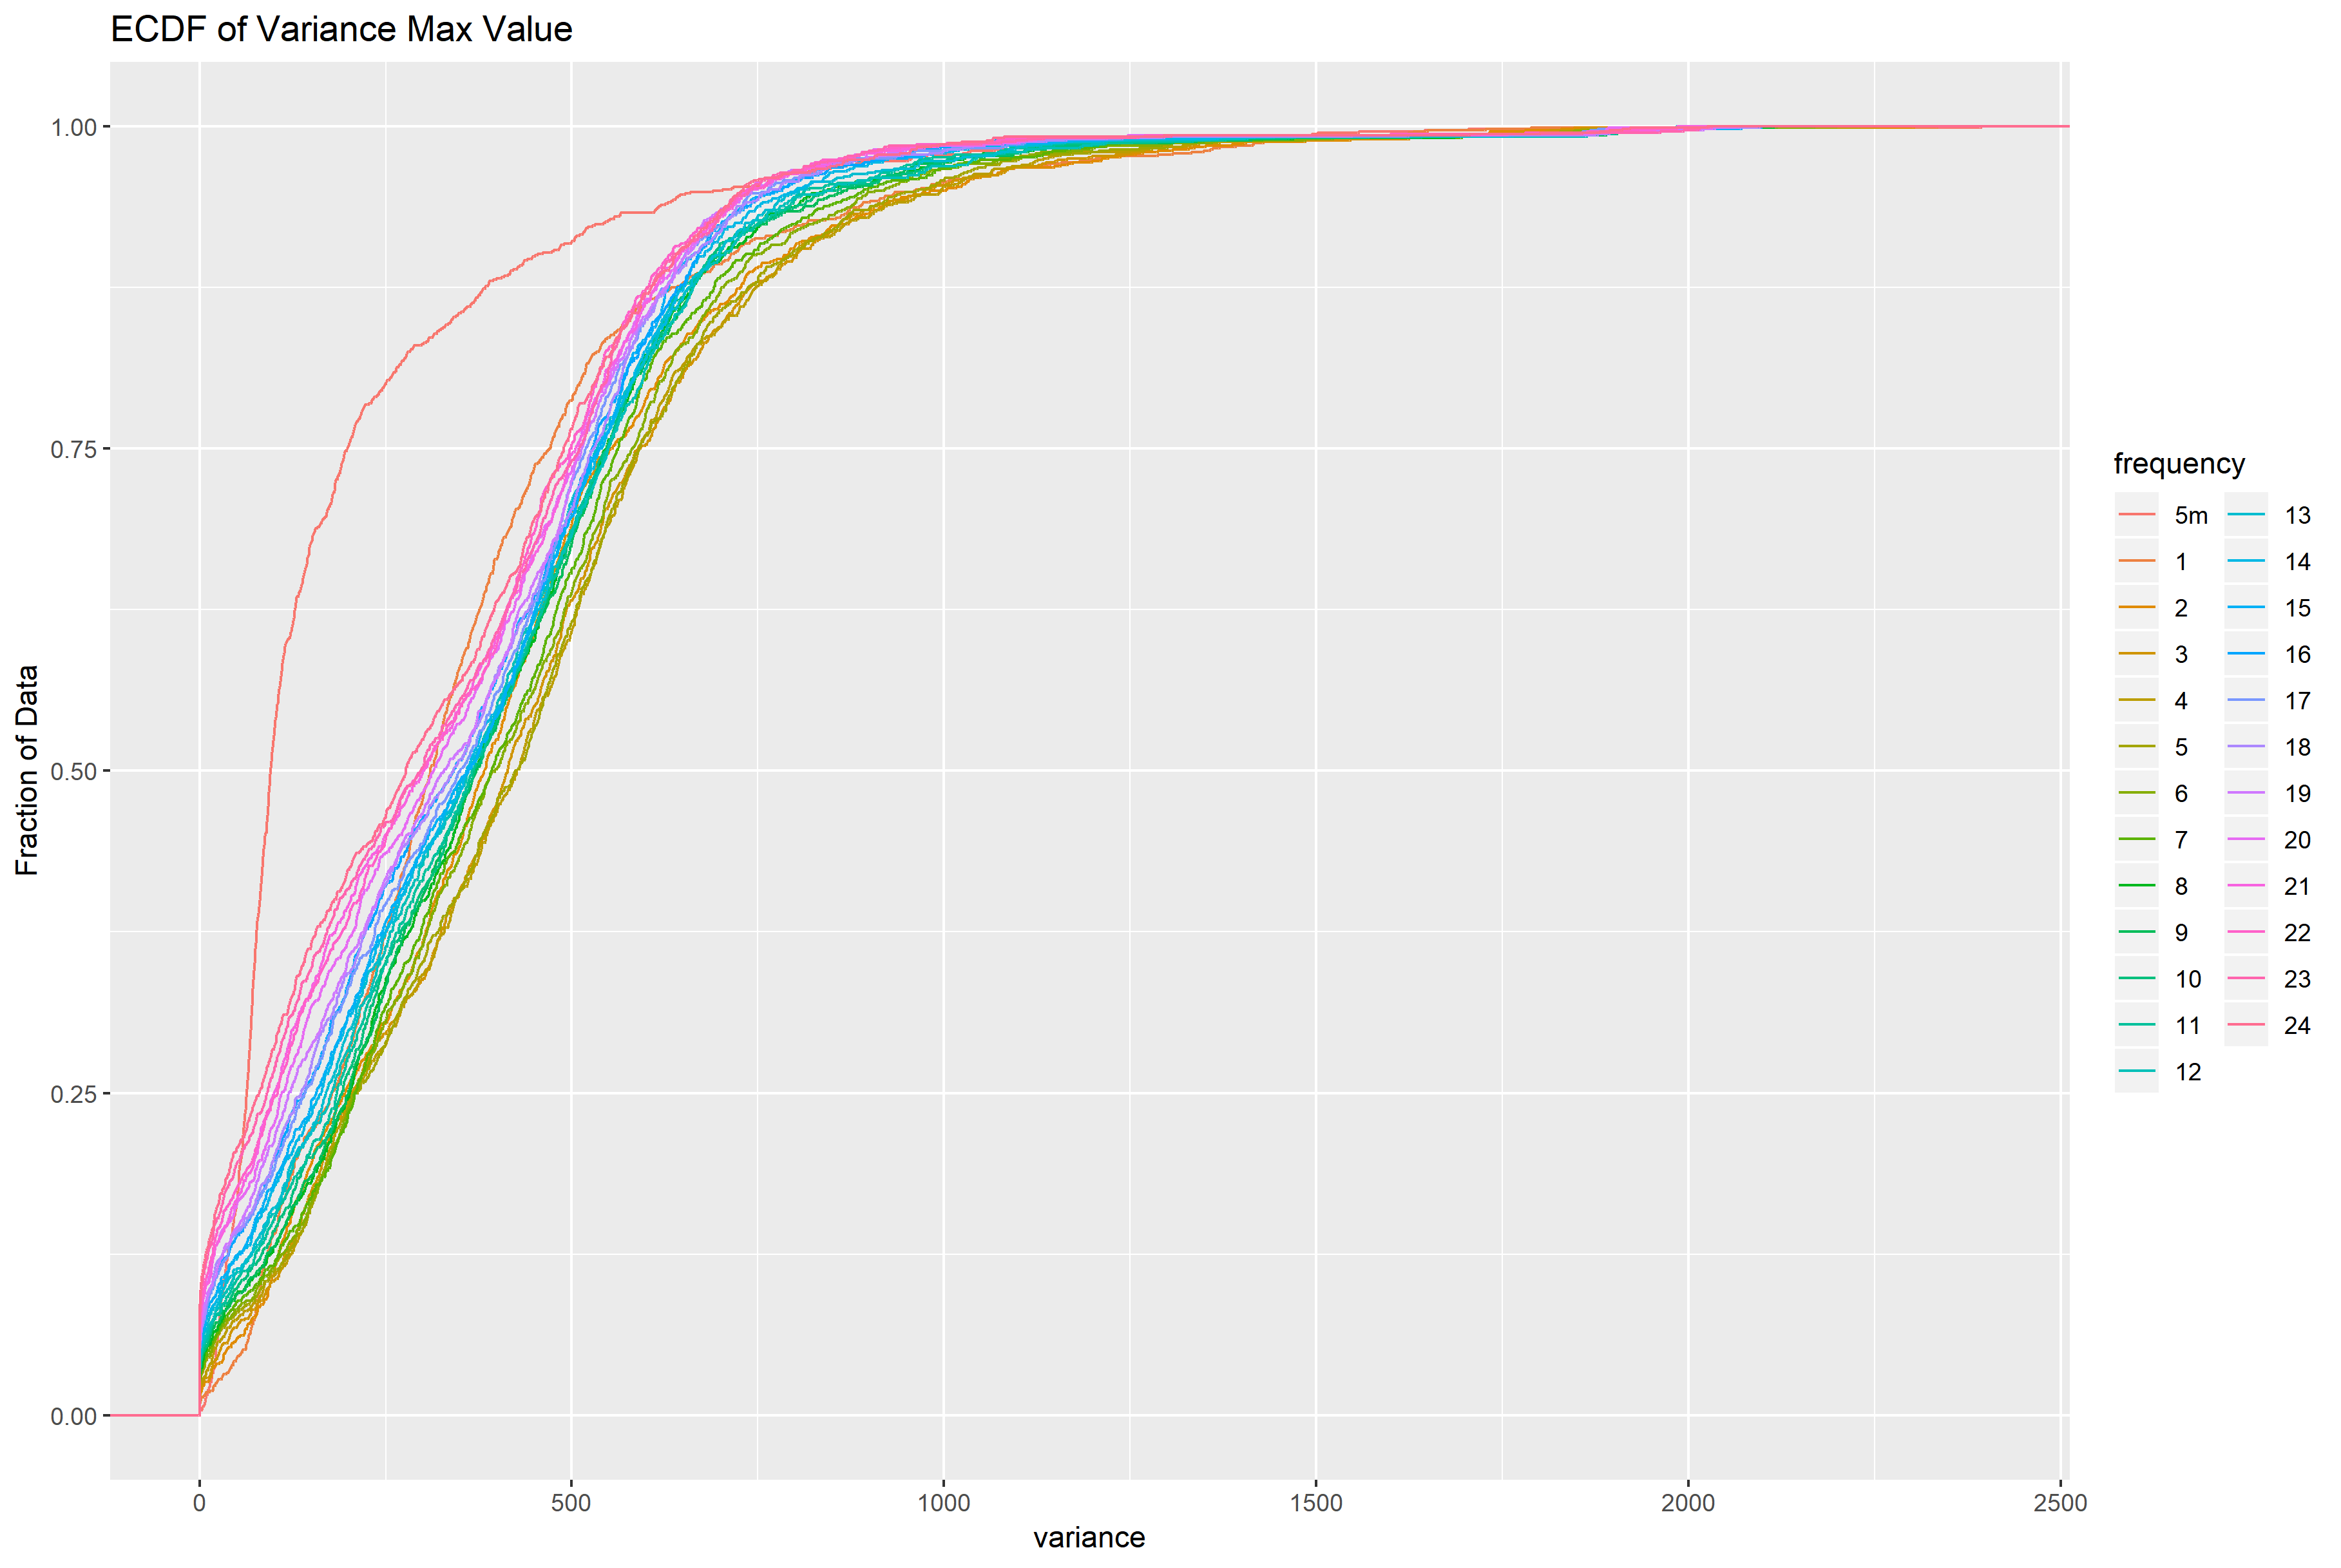
\includegraphics[width = 0.8\textwidth]{ECDFofVarianceMaxValue}
\label{fig:fig1.1.1}
\end{figure}

\begin{figure}[htbp]
\caption{ECDF of CoV of Maxes}
\centering
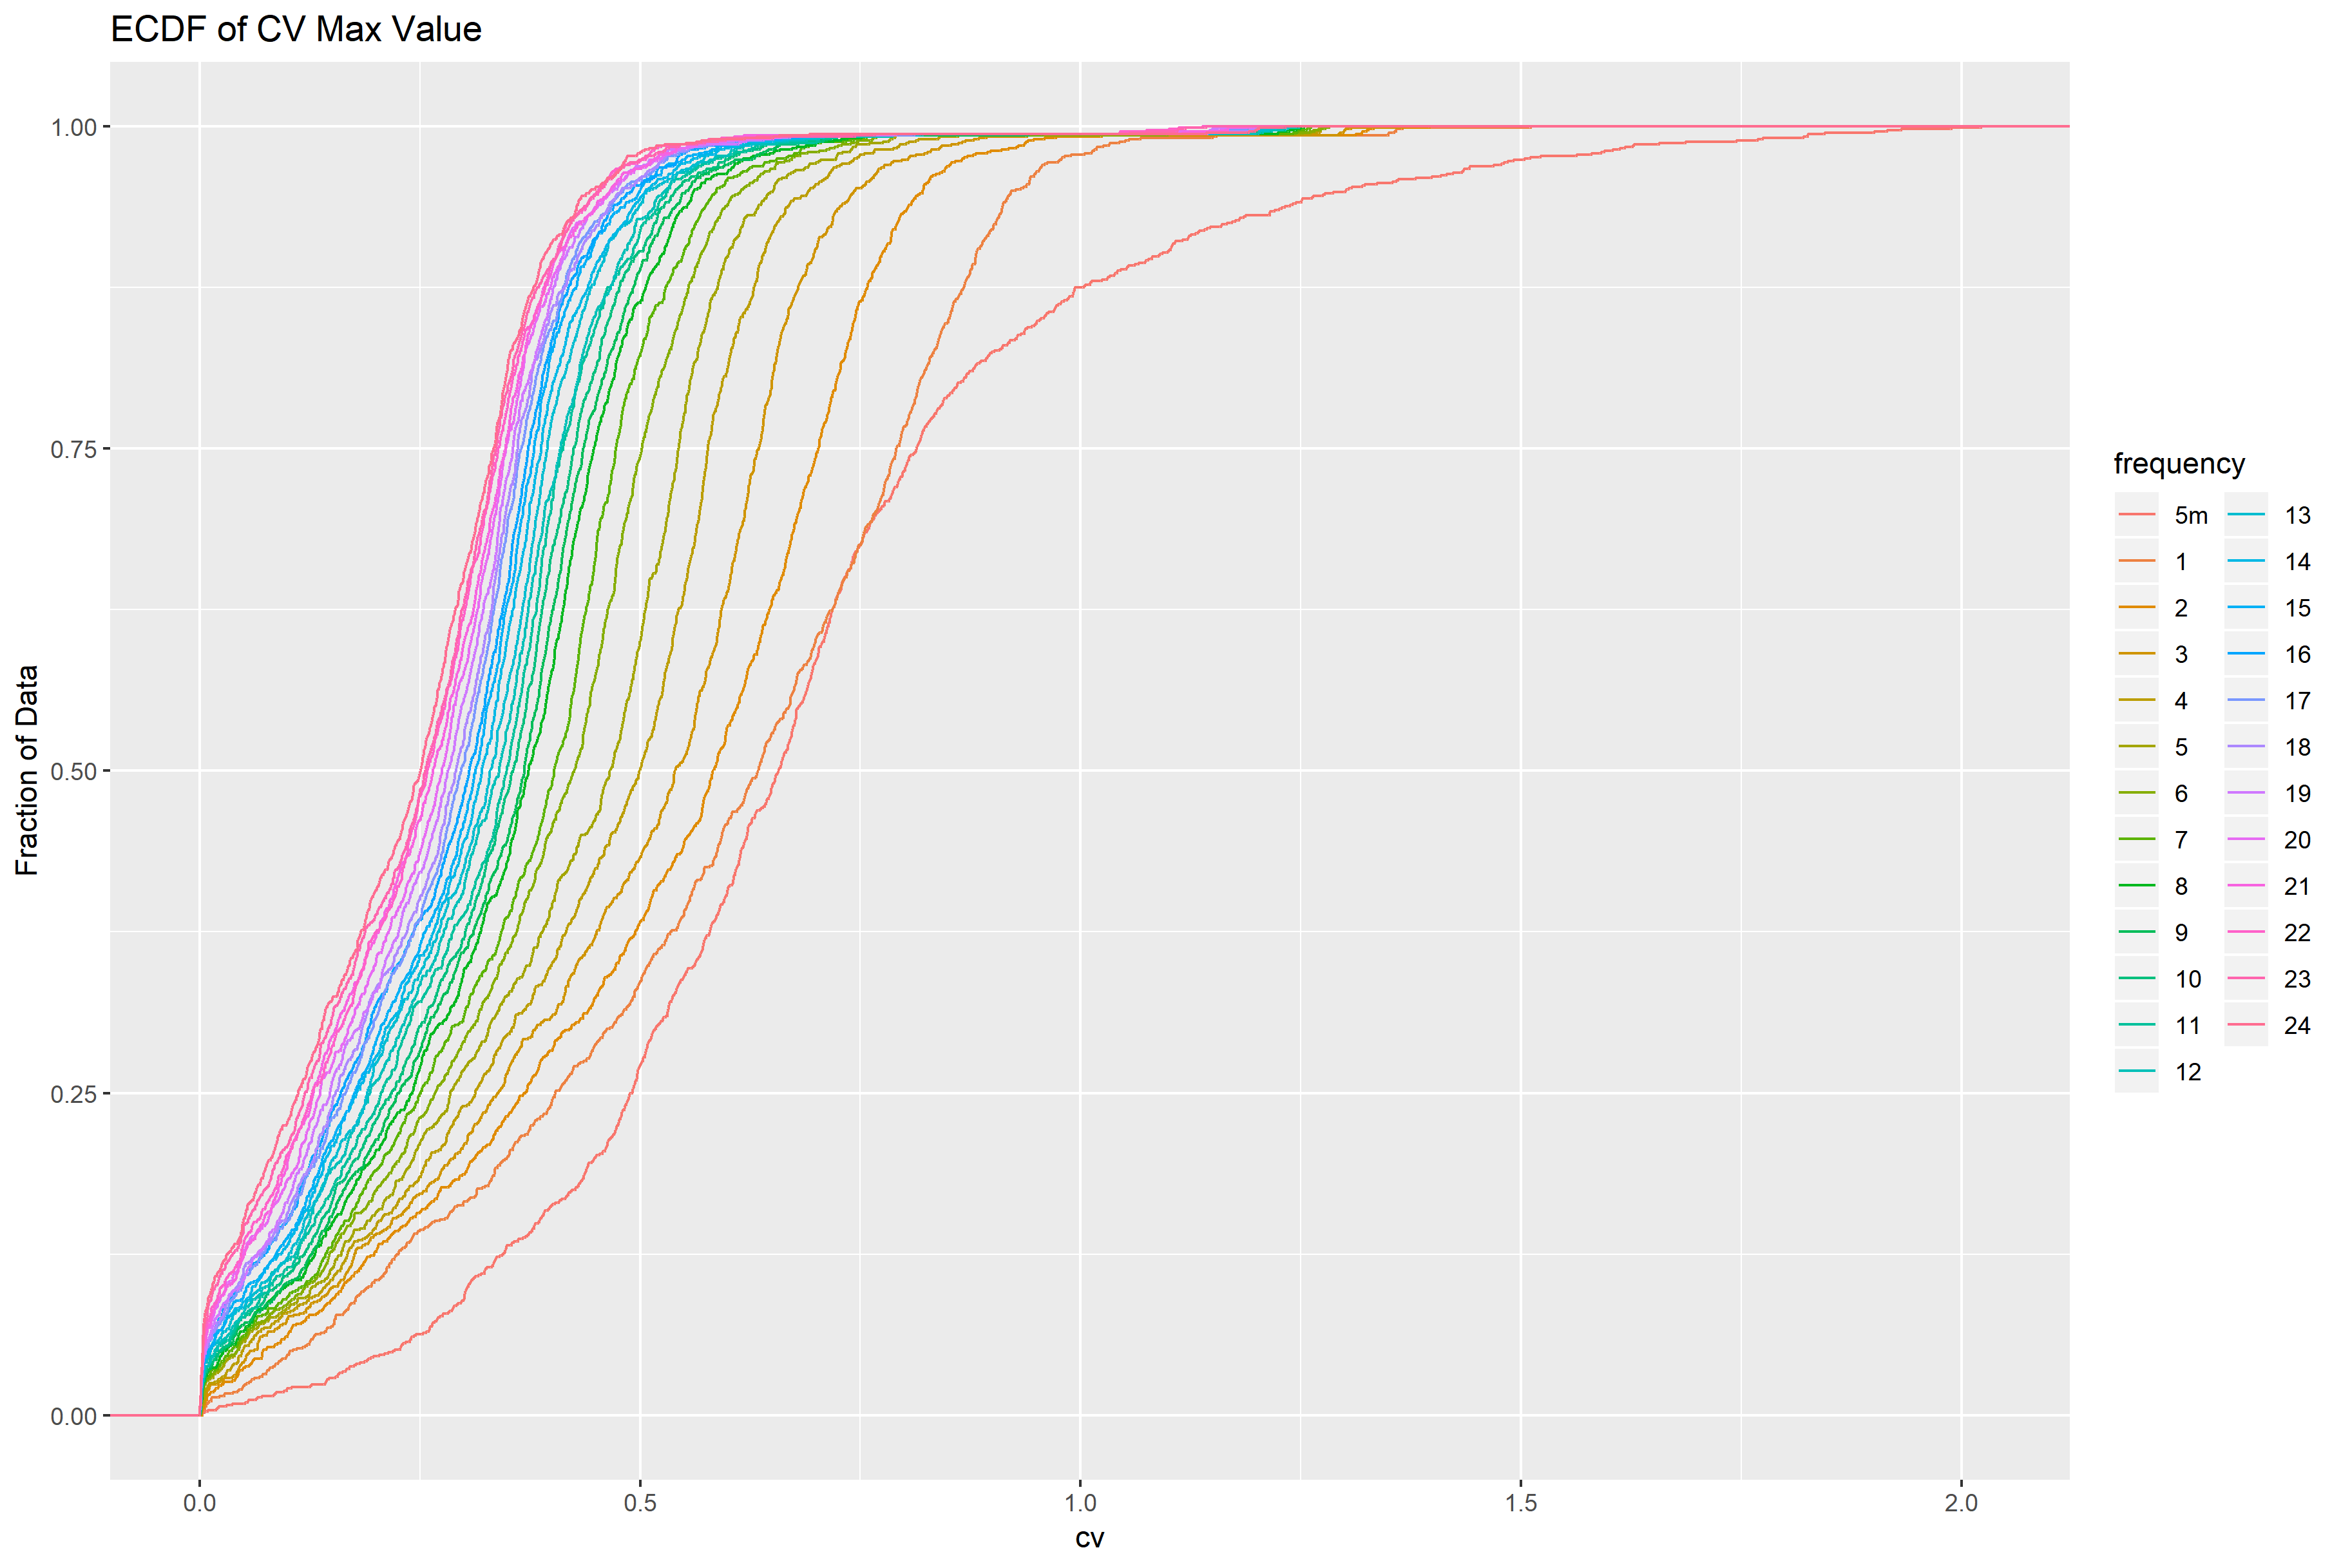
\includegraphics[width = 0.8\textwidth]{ECDFofCVMaxValue}
\label{fig:fig1.1.2}
\end{figure}

\begin{figure}[htbp]
\caption{ECDF of Entropy of Maxes}
\centering
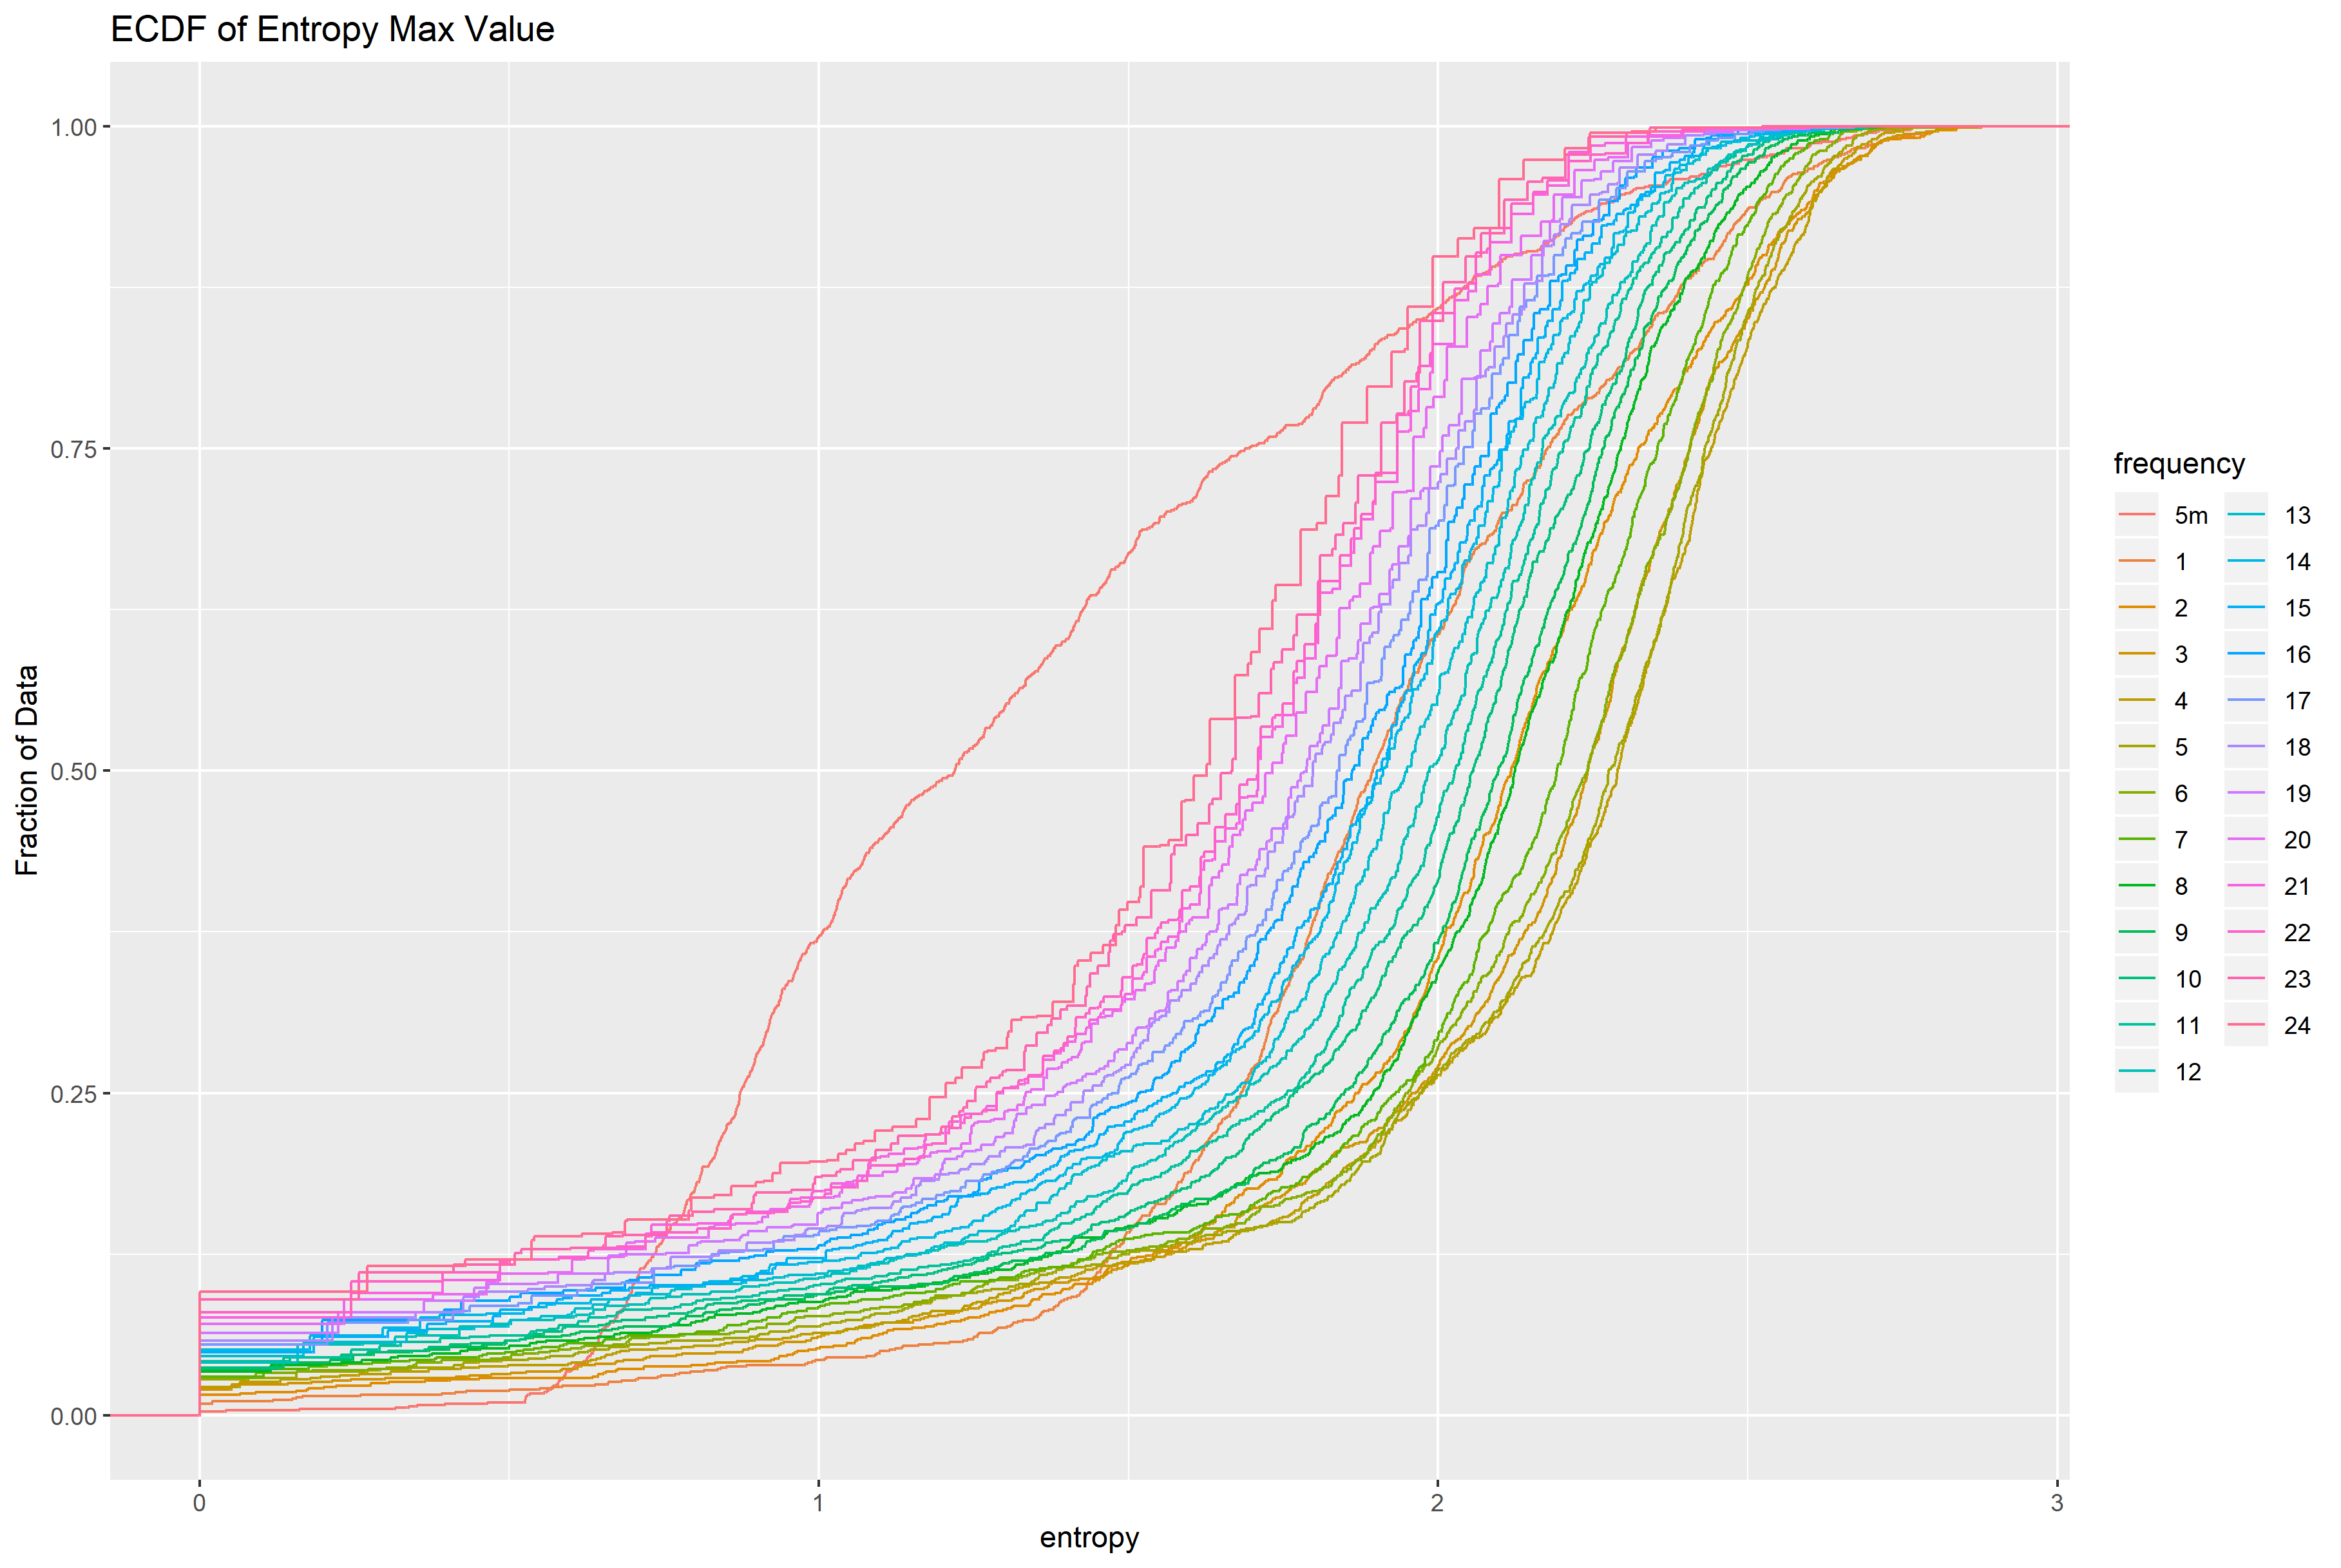
\includegraphics[width = 0.8\textwidth]{ECDFofEntropyMaxValue}
\label{fig:fig1.1.3}
\end{figure}

\begin{figure}[htbp]
\caption{ECDF of Pearson Correlation between Maxes and (Past) Maxes}
\centering
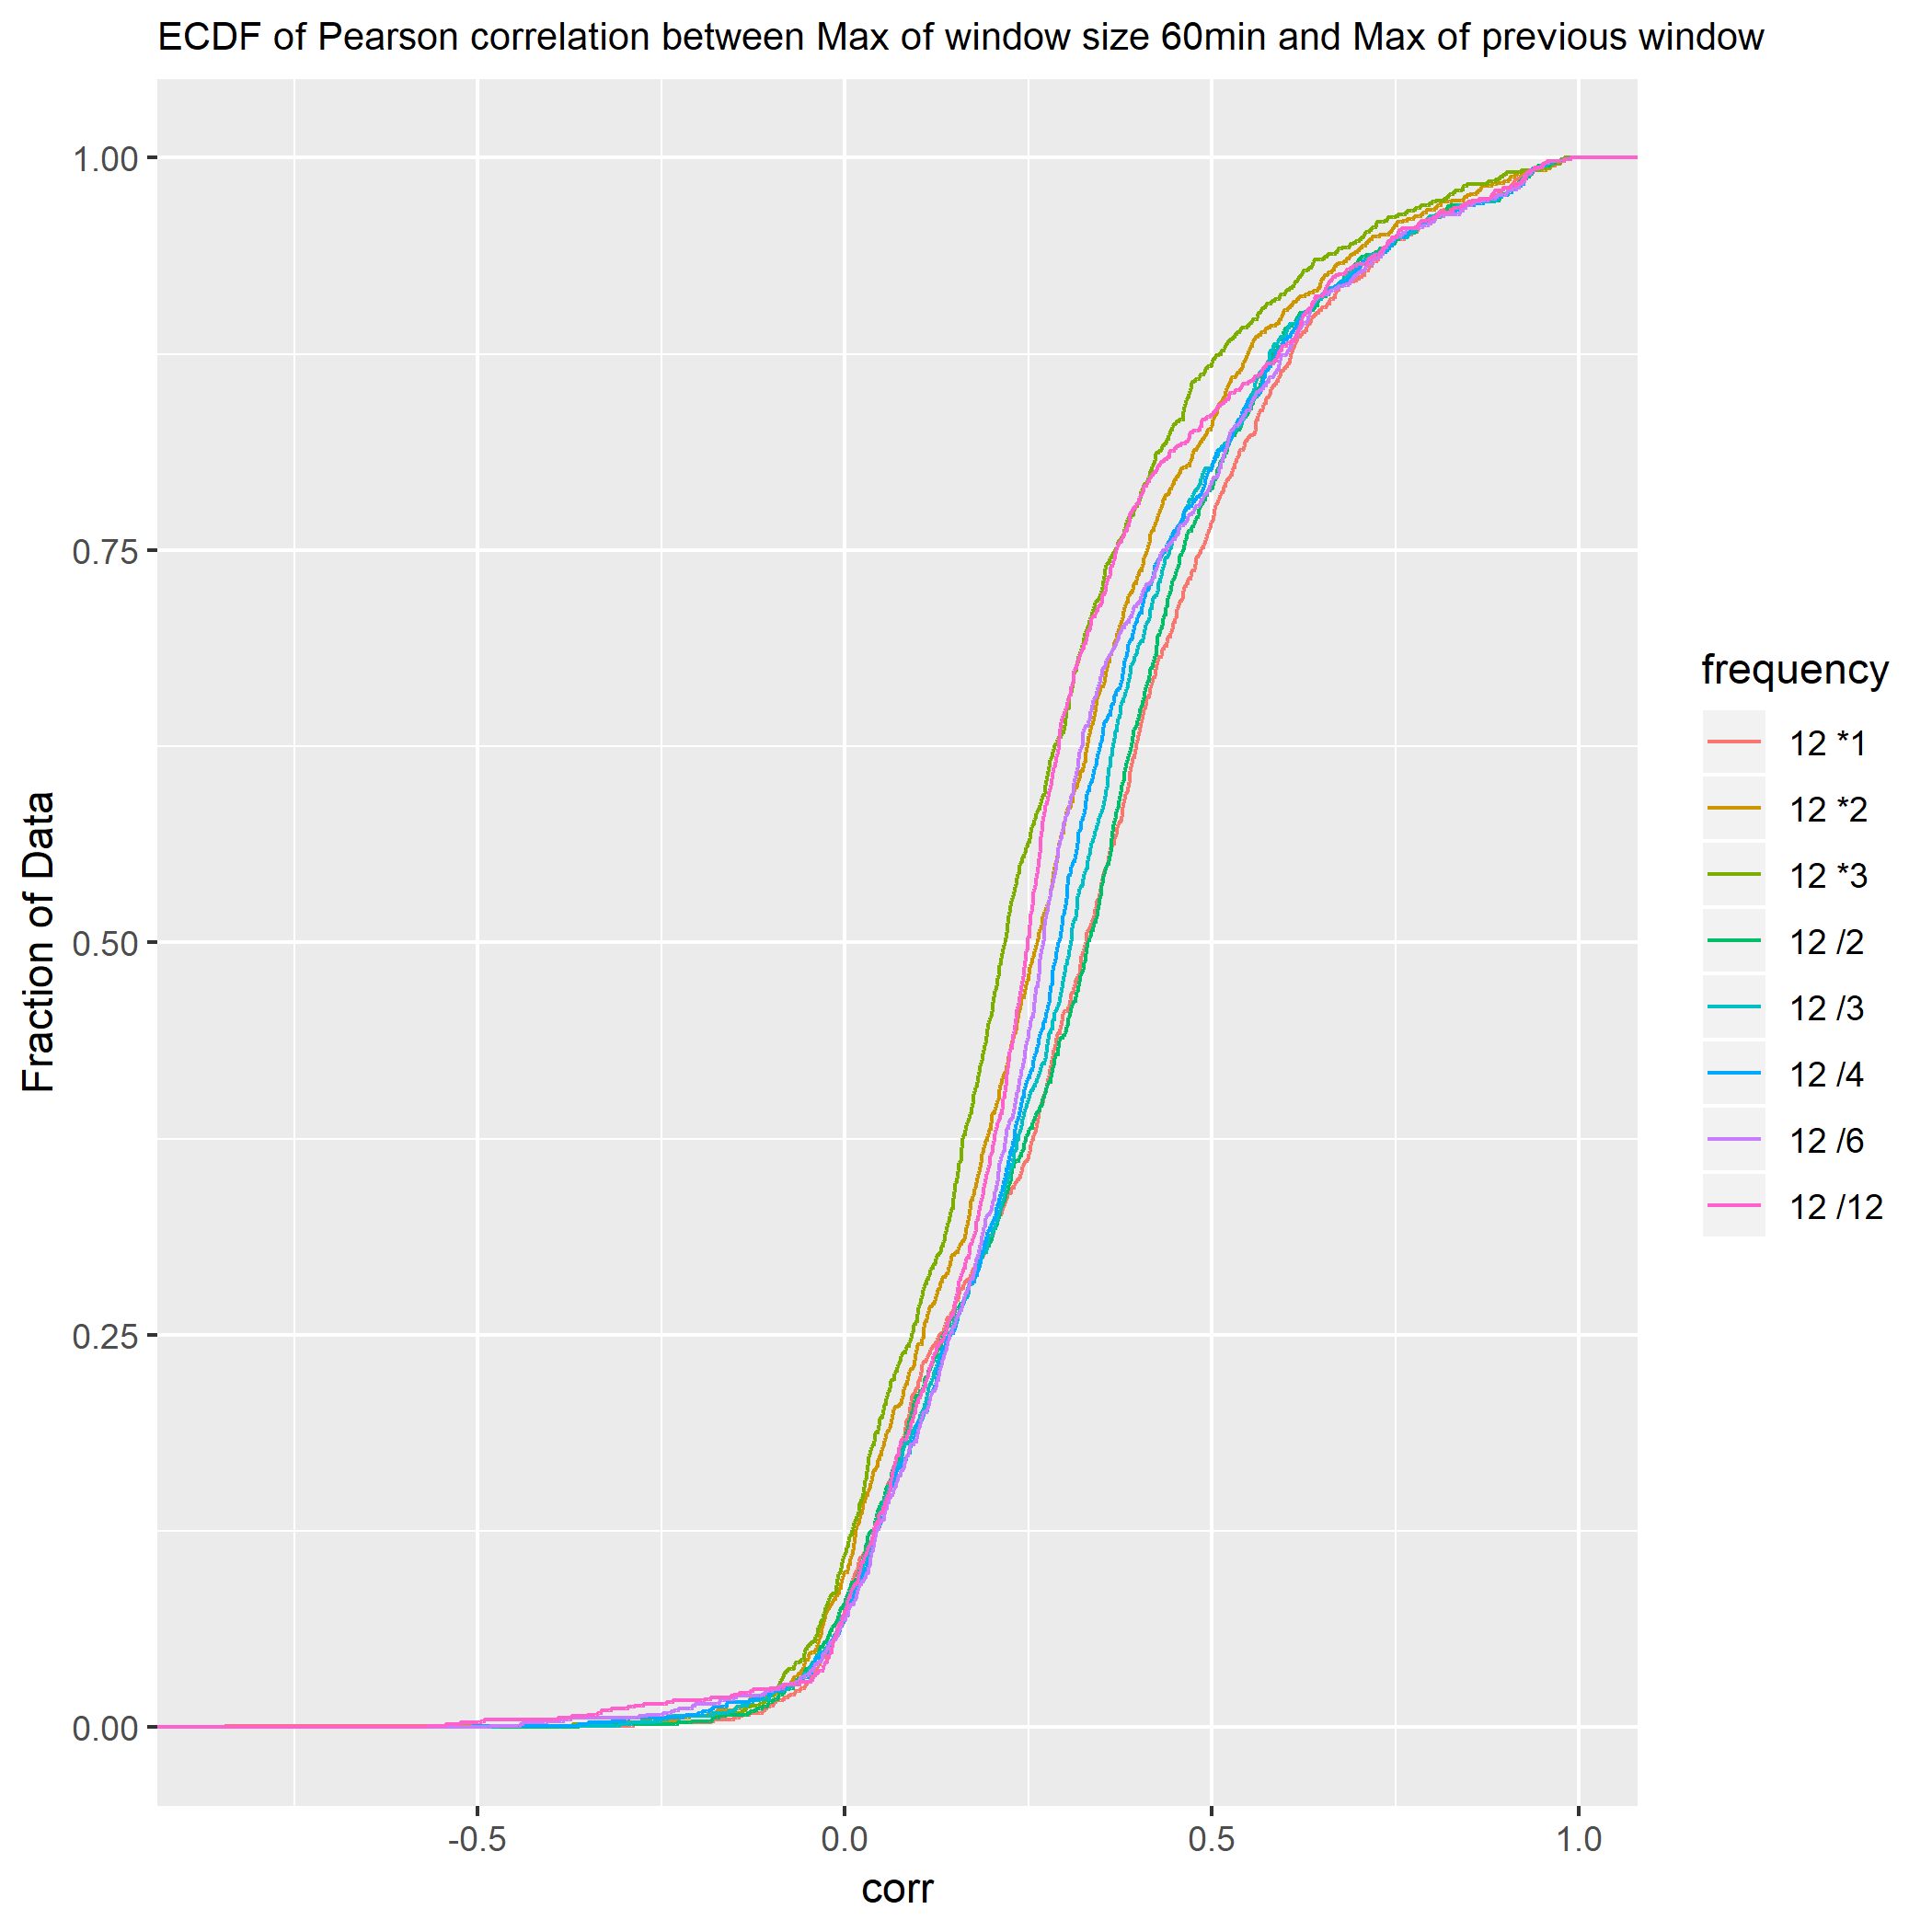
\includegraphics[width = 0.8\textwidth]{ECDFofPearsoncorrelationbetweenMaxofwindowsize60minandMaxofpreviouswindow}
\label{fig:fig1.1.4}
\end{figure}

\begin{figure}[htbp]
\caption{ECDF of Pearson Correlation between Maxes and (Past) Avgs}
\centering
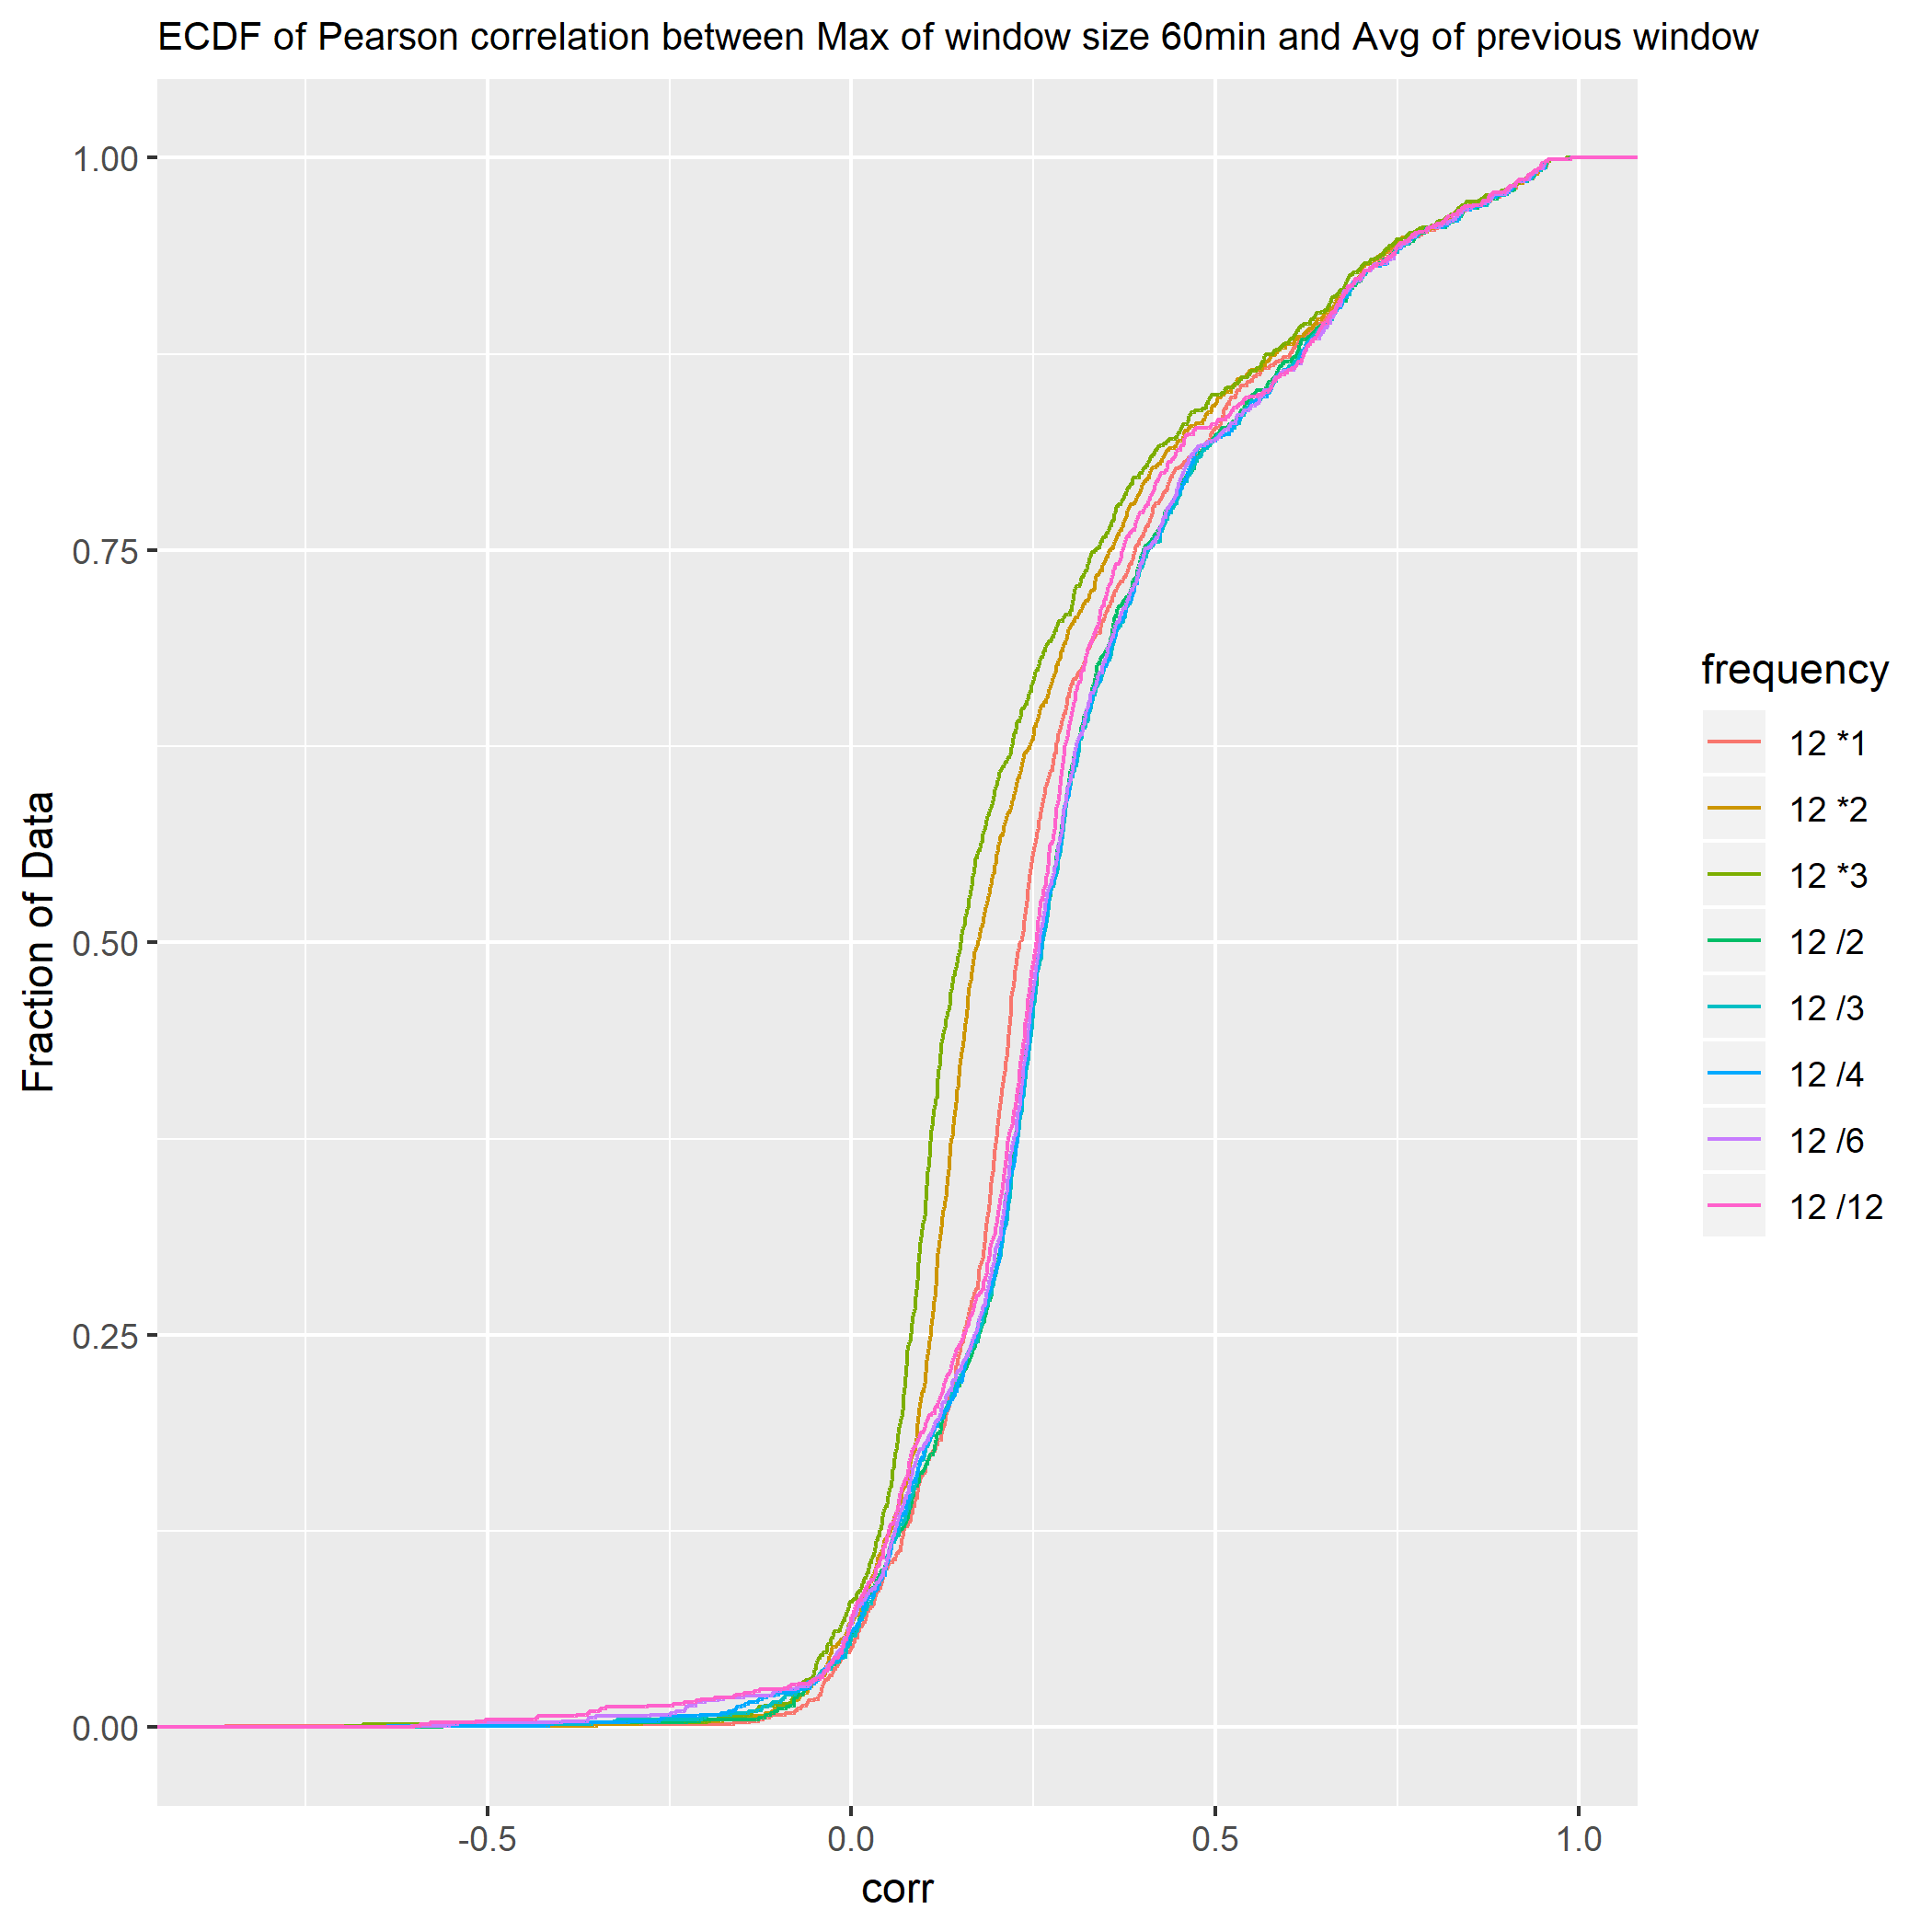
\includegraphics[width = 0.8\textwidth]{ECDFofPearsoncorrelationbetweenMaxofwindowsize60minandAvgofpreviouswindow}
\label{fig:fig1.1.5}
\end{figure}

\begin{figure}[htbp]
\caption{ECDF of Pearson Correlation between Maxes and (Past) Average of Maxes}
\centering
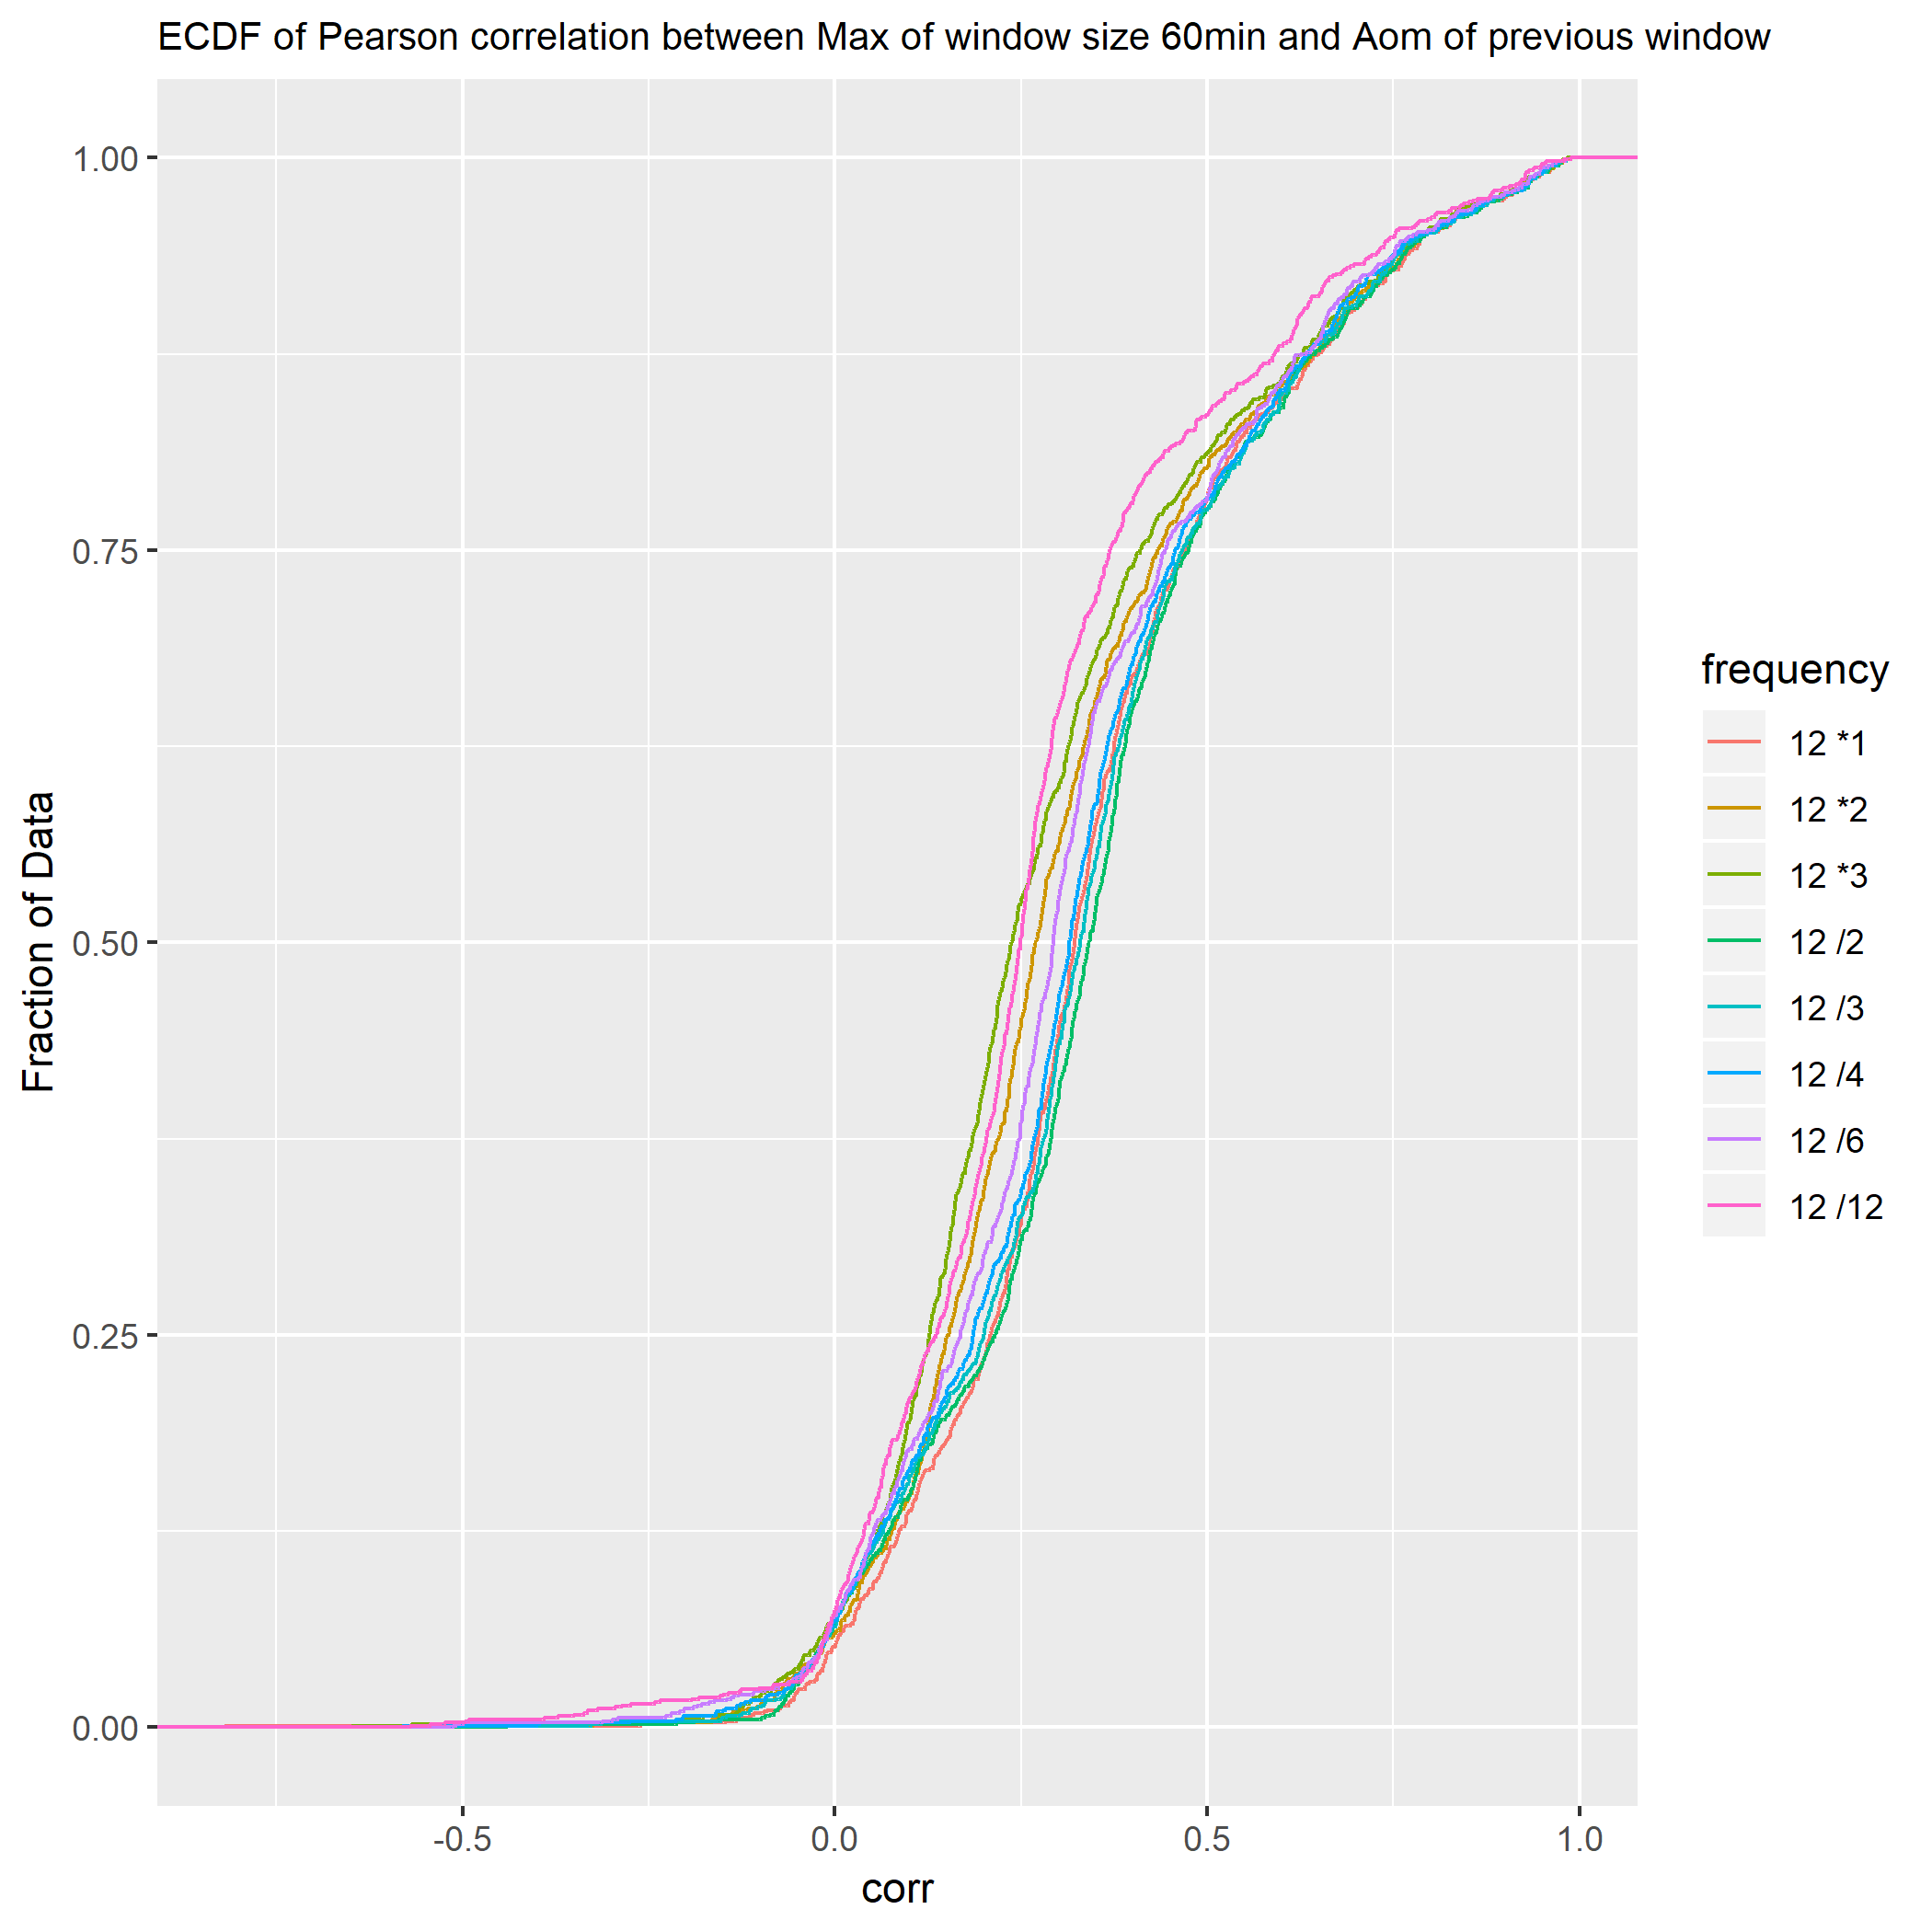
\includegraphics[width = 0.8\textwidth]{ECDFofPearsoncorrelationbetweenMaxofwindowsize60minandAomofpreviouswindow}
\label{fig:fig1.1.6}
\end{figure}

\subsubsection{Models}
Ref to Section 1.3, include Fig \ref{fig:fig1.3.1}, Table \ref{tab:tab1.3.1}, Fig \ref{fig:fig1.3.2}, Table \ref{tab:tab1.3.2}, Fig \ref{fig:fig1.3.3}, Table \ref{tab:tab1.3.3}, Fig \ref{fig:fig1.3.4}, Table \ref{tab:tab1.3.4}, Table \ref{fig:fig1.3.5}, Table \ref{tab:tab1.3.5}, Table \ref{fig:fig1.3.6}, Table \ref{tab:tab1.3.6}.

\begin{figure}[htbp]
\caption{ECDF of Scores for AR1,AR1X Models with Offline Training}
\centering
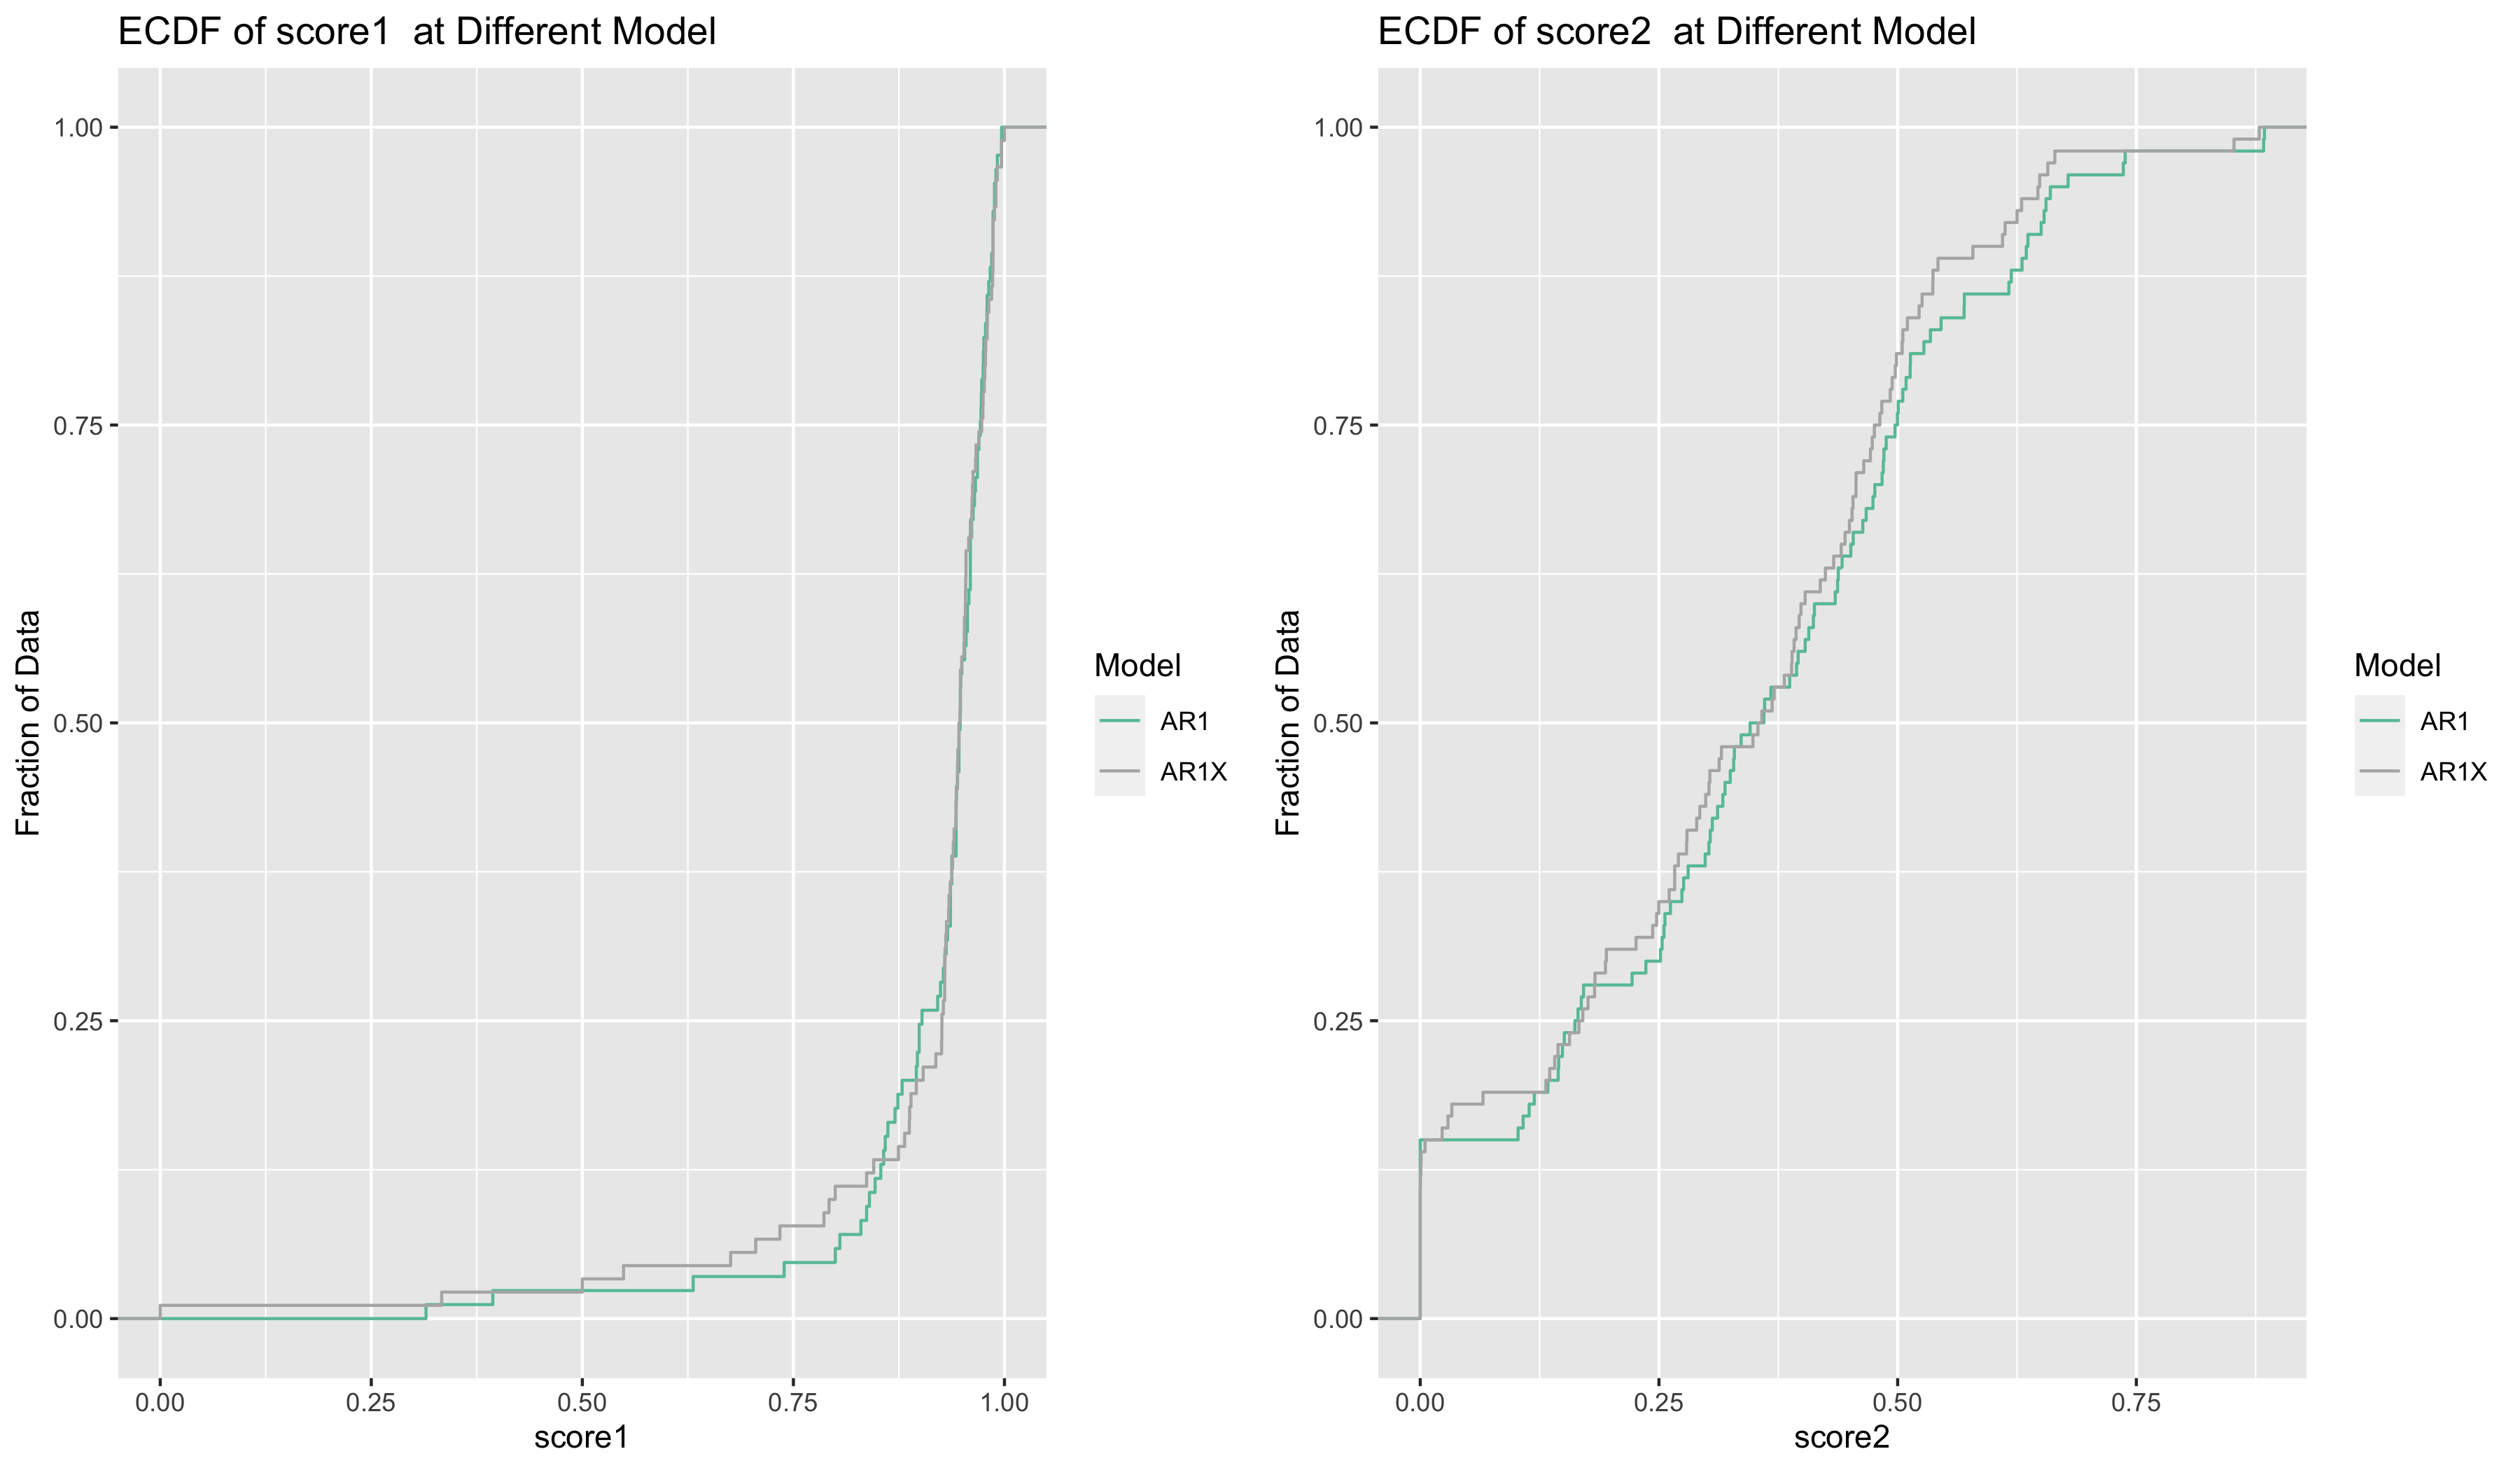
\includegraphics[width = 0.8\textwidth]{images/ECDFofscoresatDifferentModelOfAR1, AR1X.png}
\label{fig:fig1.3.1}

\end{figure}

\begin{table}[htbp]
  \begin{center}
    \caption{Configuration and Result of AR1,AR1X Models with Offline Training}
    \label{tab:tab1.3.1}
    \begin{tabular}{l|*{4}{c}}
      \textbf{name} & \textbf{score 1} & \textbf{score 1 weight} & \textbf{score 2} & \textbf{score 2 weight} \\
      \hline
      AR1 & 0.9168 & 48124 & 0.3463 & 59249\\
      AR1X & 0.9293 & 45094 & 0.3270 & 59249\\
    \end{tabular}
  \end{center}
\end{table}

\begin{figure}[htbp]
\caption{ECDF of Scores for ARI,AUTO ARIMA Models with Offline Training}
\centering
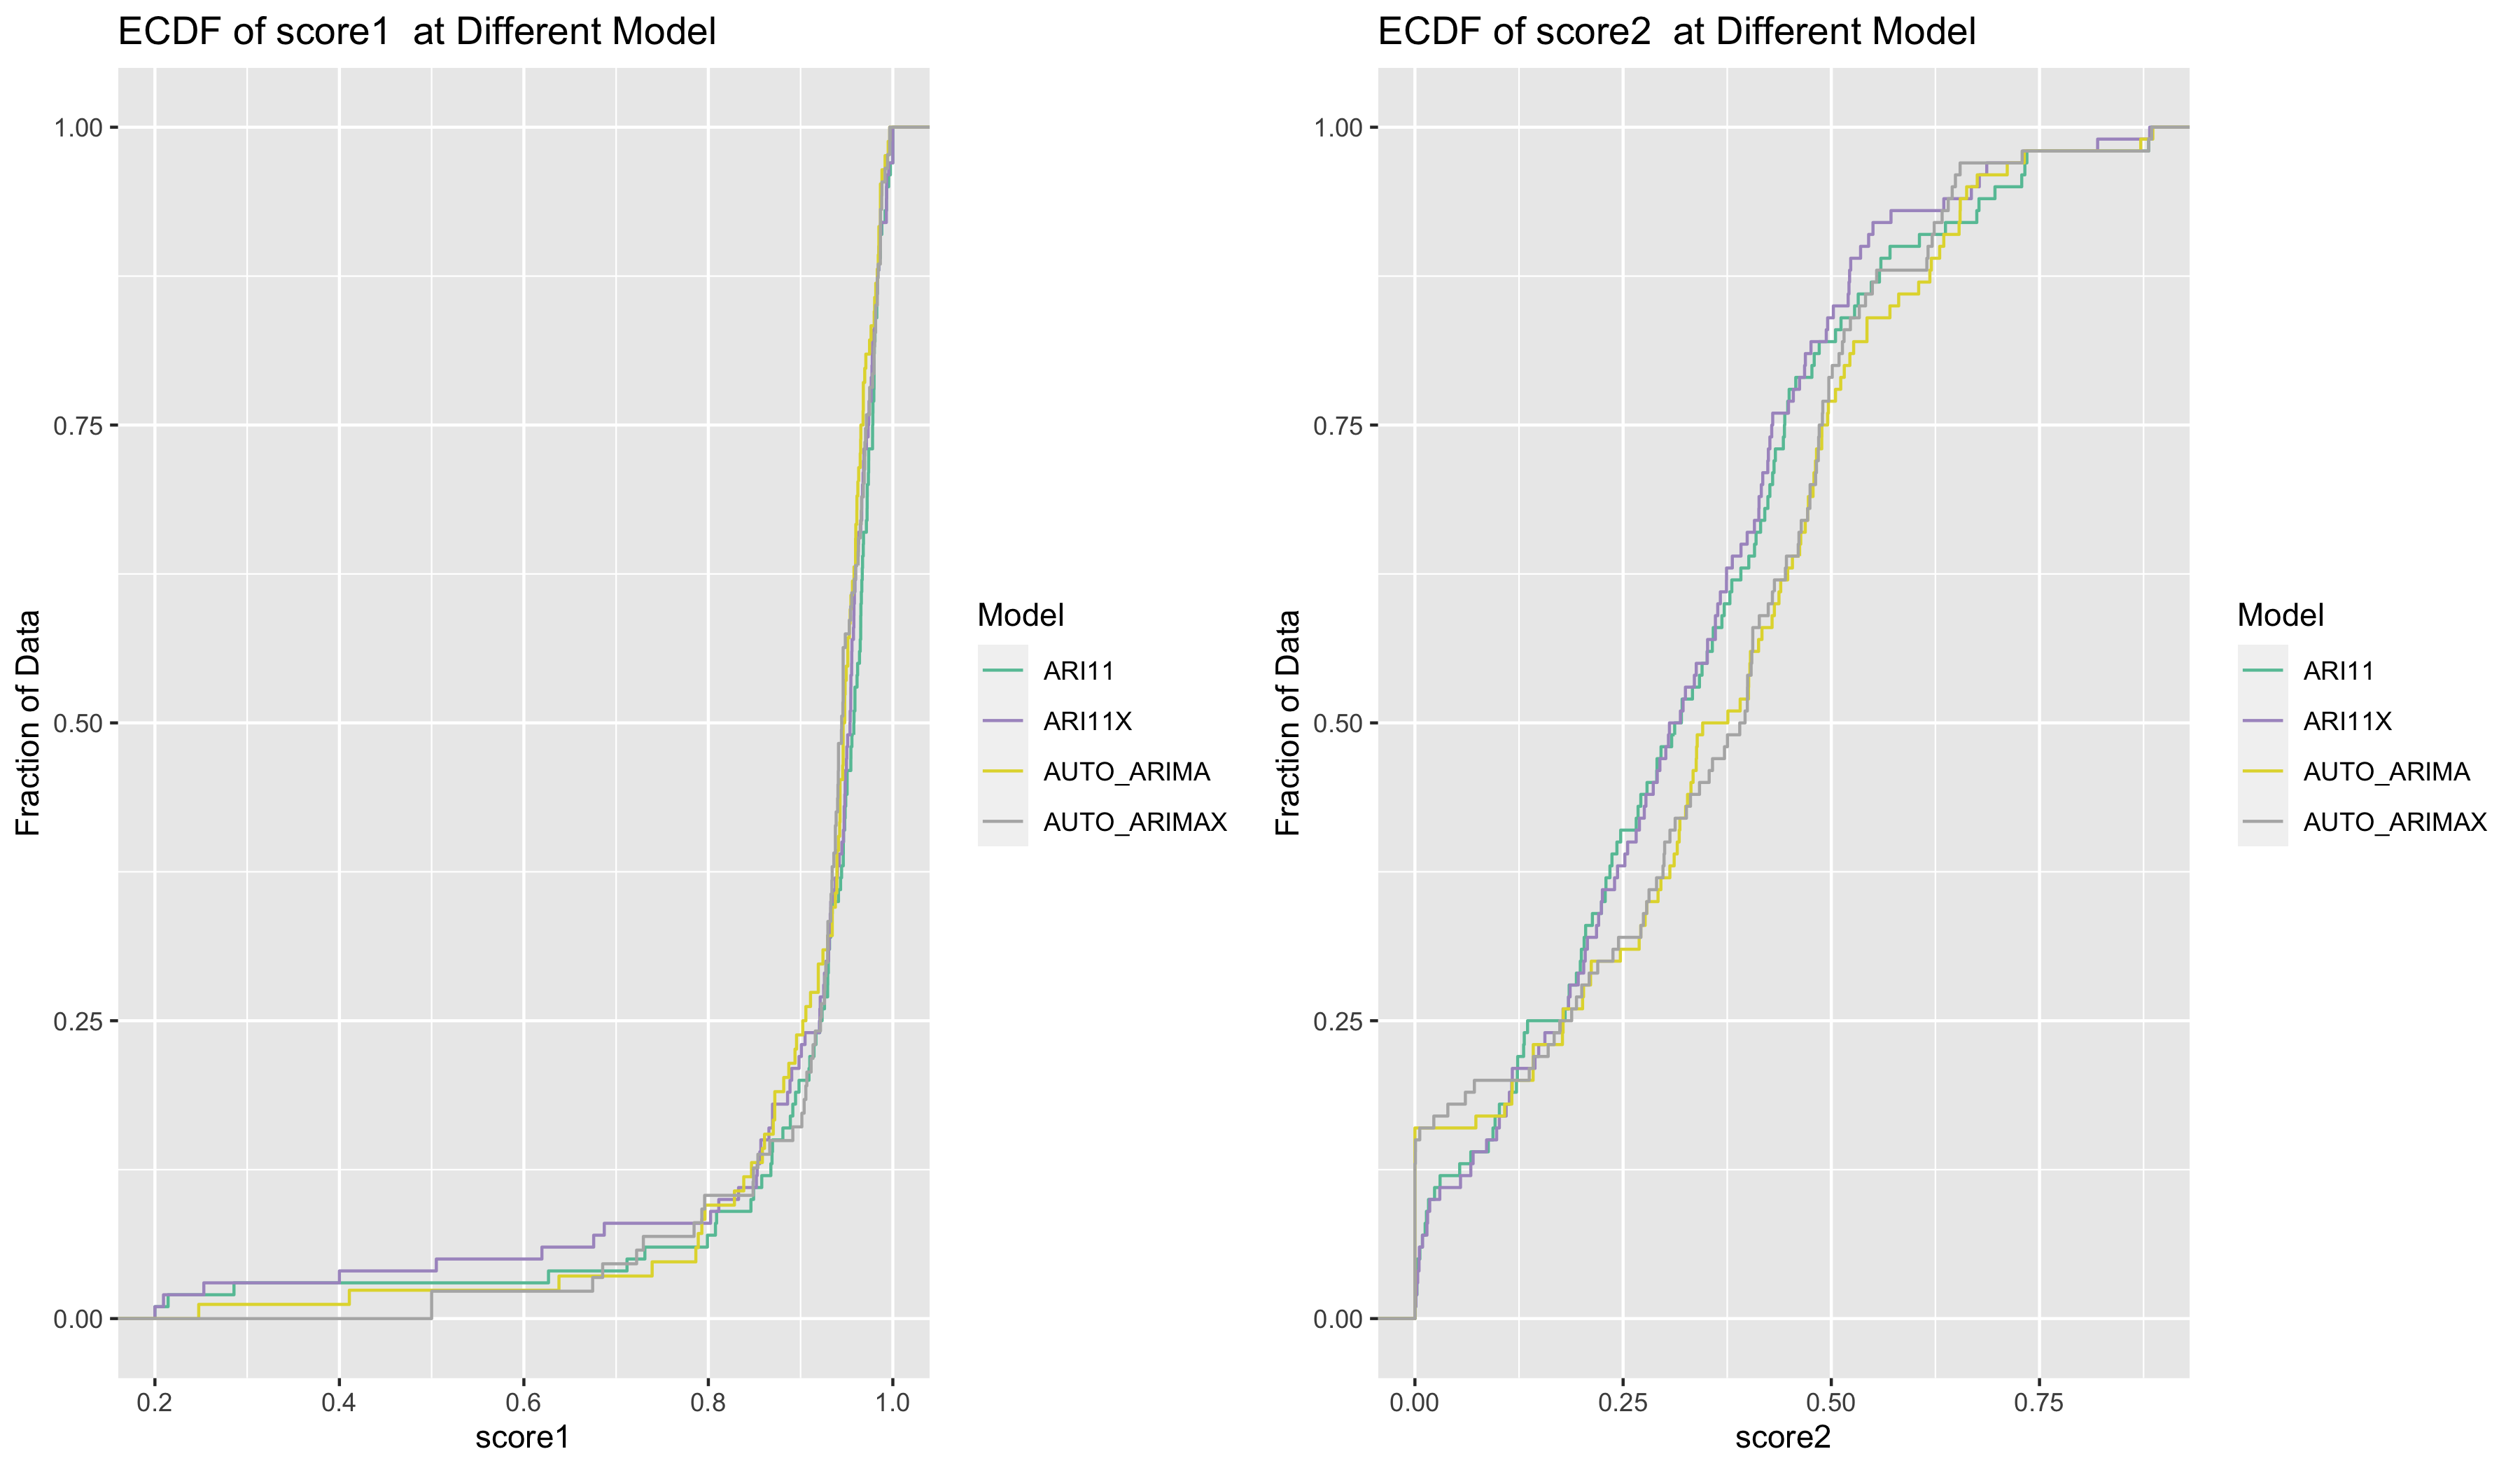
\includegraphics[width = 0.8\textwidth]{images/ECDFofscoresatDifferentModelOfARI11, ARI11X, AUTOARIMA, AUTOARIMAX.png}
\label{fig:fig1.3.2}
\end{figure}

\begin{table}[htbp]
  \begin{center}
    \caption{Configuration and Result of AR1,AR1X Models with Offline Training}
    \label{tab:tab1.3.2}
    \begin{tabular}{l|*{4}{c}}
      \textbf{name} & \textbf{score 1} & \textbf{score 1 weight} & \textbf{score 2} & \textbf{score 2 weight} \\
      \hline
      ARI11 & 0.9410 & 46307 & 0.3205 & 59249\\
      ARI11X & 0.9238 & 45778 & 0.3140 & 59249\\
      AUTO & 0.9135 & 47882 & 0.3494 & 59249\\
      AUTOX & 0.9295 & 45323 & 0.3423 & 59249\\
    \end{tabular}
  \end{center}
\end{table}

\begin{figure}[htbp]
\caption{ECDF of Scores for AR1 with Different Residual Distribution Estimation}
\centering
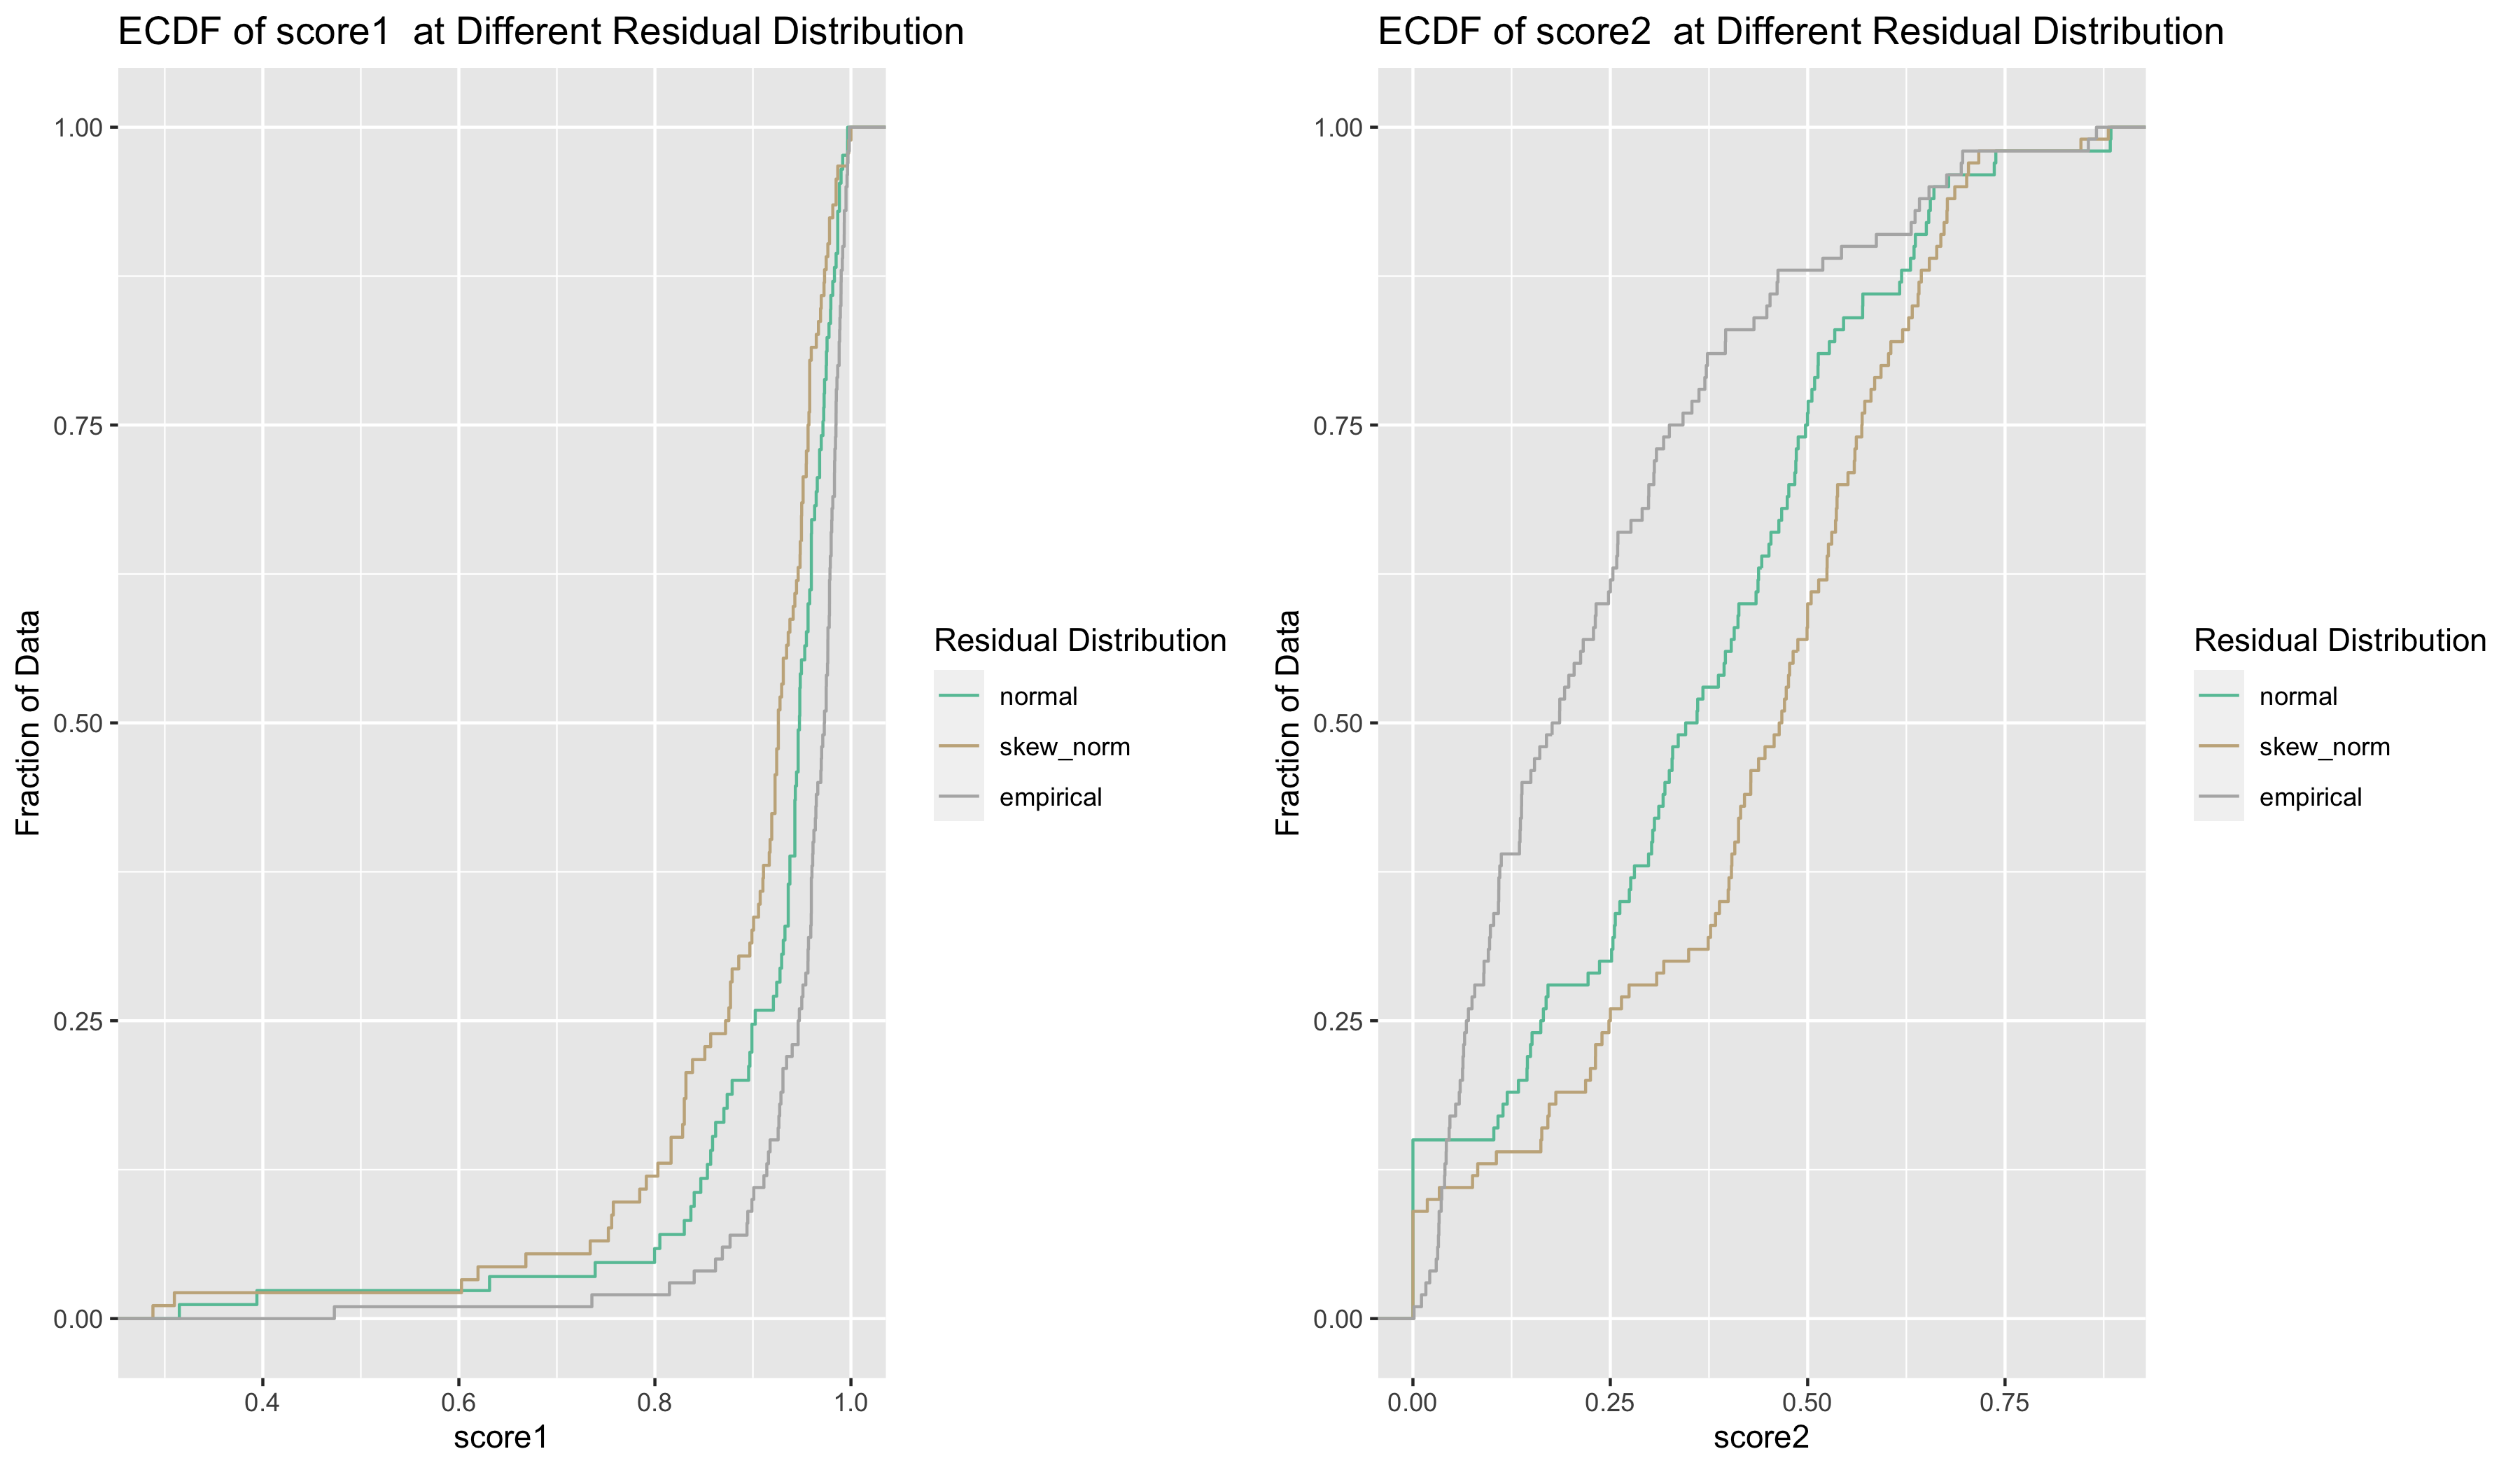
\includegraphics[width = 0.8\textwidth]{images/ECDFofscoresatDifferentResidualDistributionOfAR1,840,1,3.png}
\label{fig:fig1.3.3}
\end{figure}

\begin{table}[htbp]
  \begin{center}
    \caption{Configuration and Result of AR1 Model with Different Residual Distribution Estimation}
    \label{tab:tab1.3.3}
    \begin{tabular}{l|*{4}{c}}
      \textbf{residual distribution} & \textbf{score 1} & \textbf{score 1 weight} & \textbf{score 2} & \textbf{score 2 weight} \\
      \hline
      Normal & 0.9168 & 48124 & 0.3463 & 59249\\
      Skew-normal & 0.8881 & 51728 & 0.4163 & 59249\\
      Empirical & 0.9519 & 50756 & 0.2362 & 59249\\
    \end{tabular}
  \end{center}
\end{table}

\begin{figure}[htbp]
\caption{ECDF of Scores for AR1 with Different Outlier Detections}
\centering
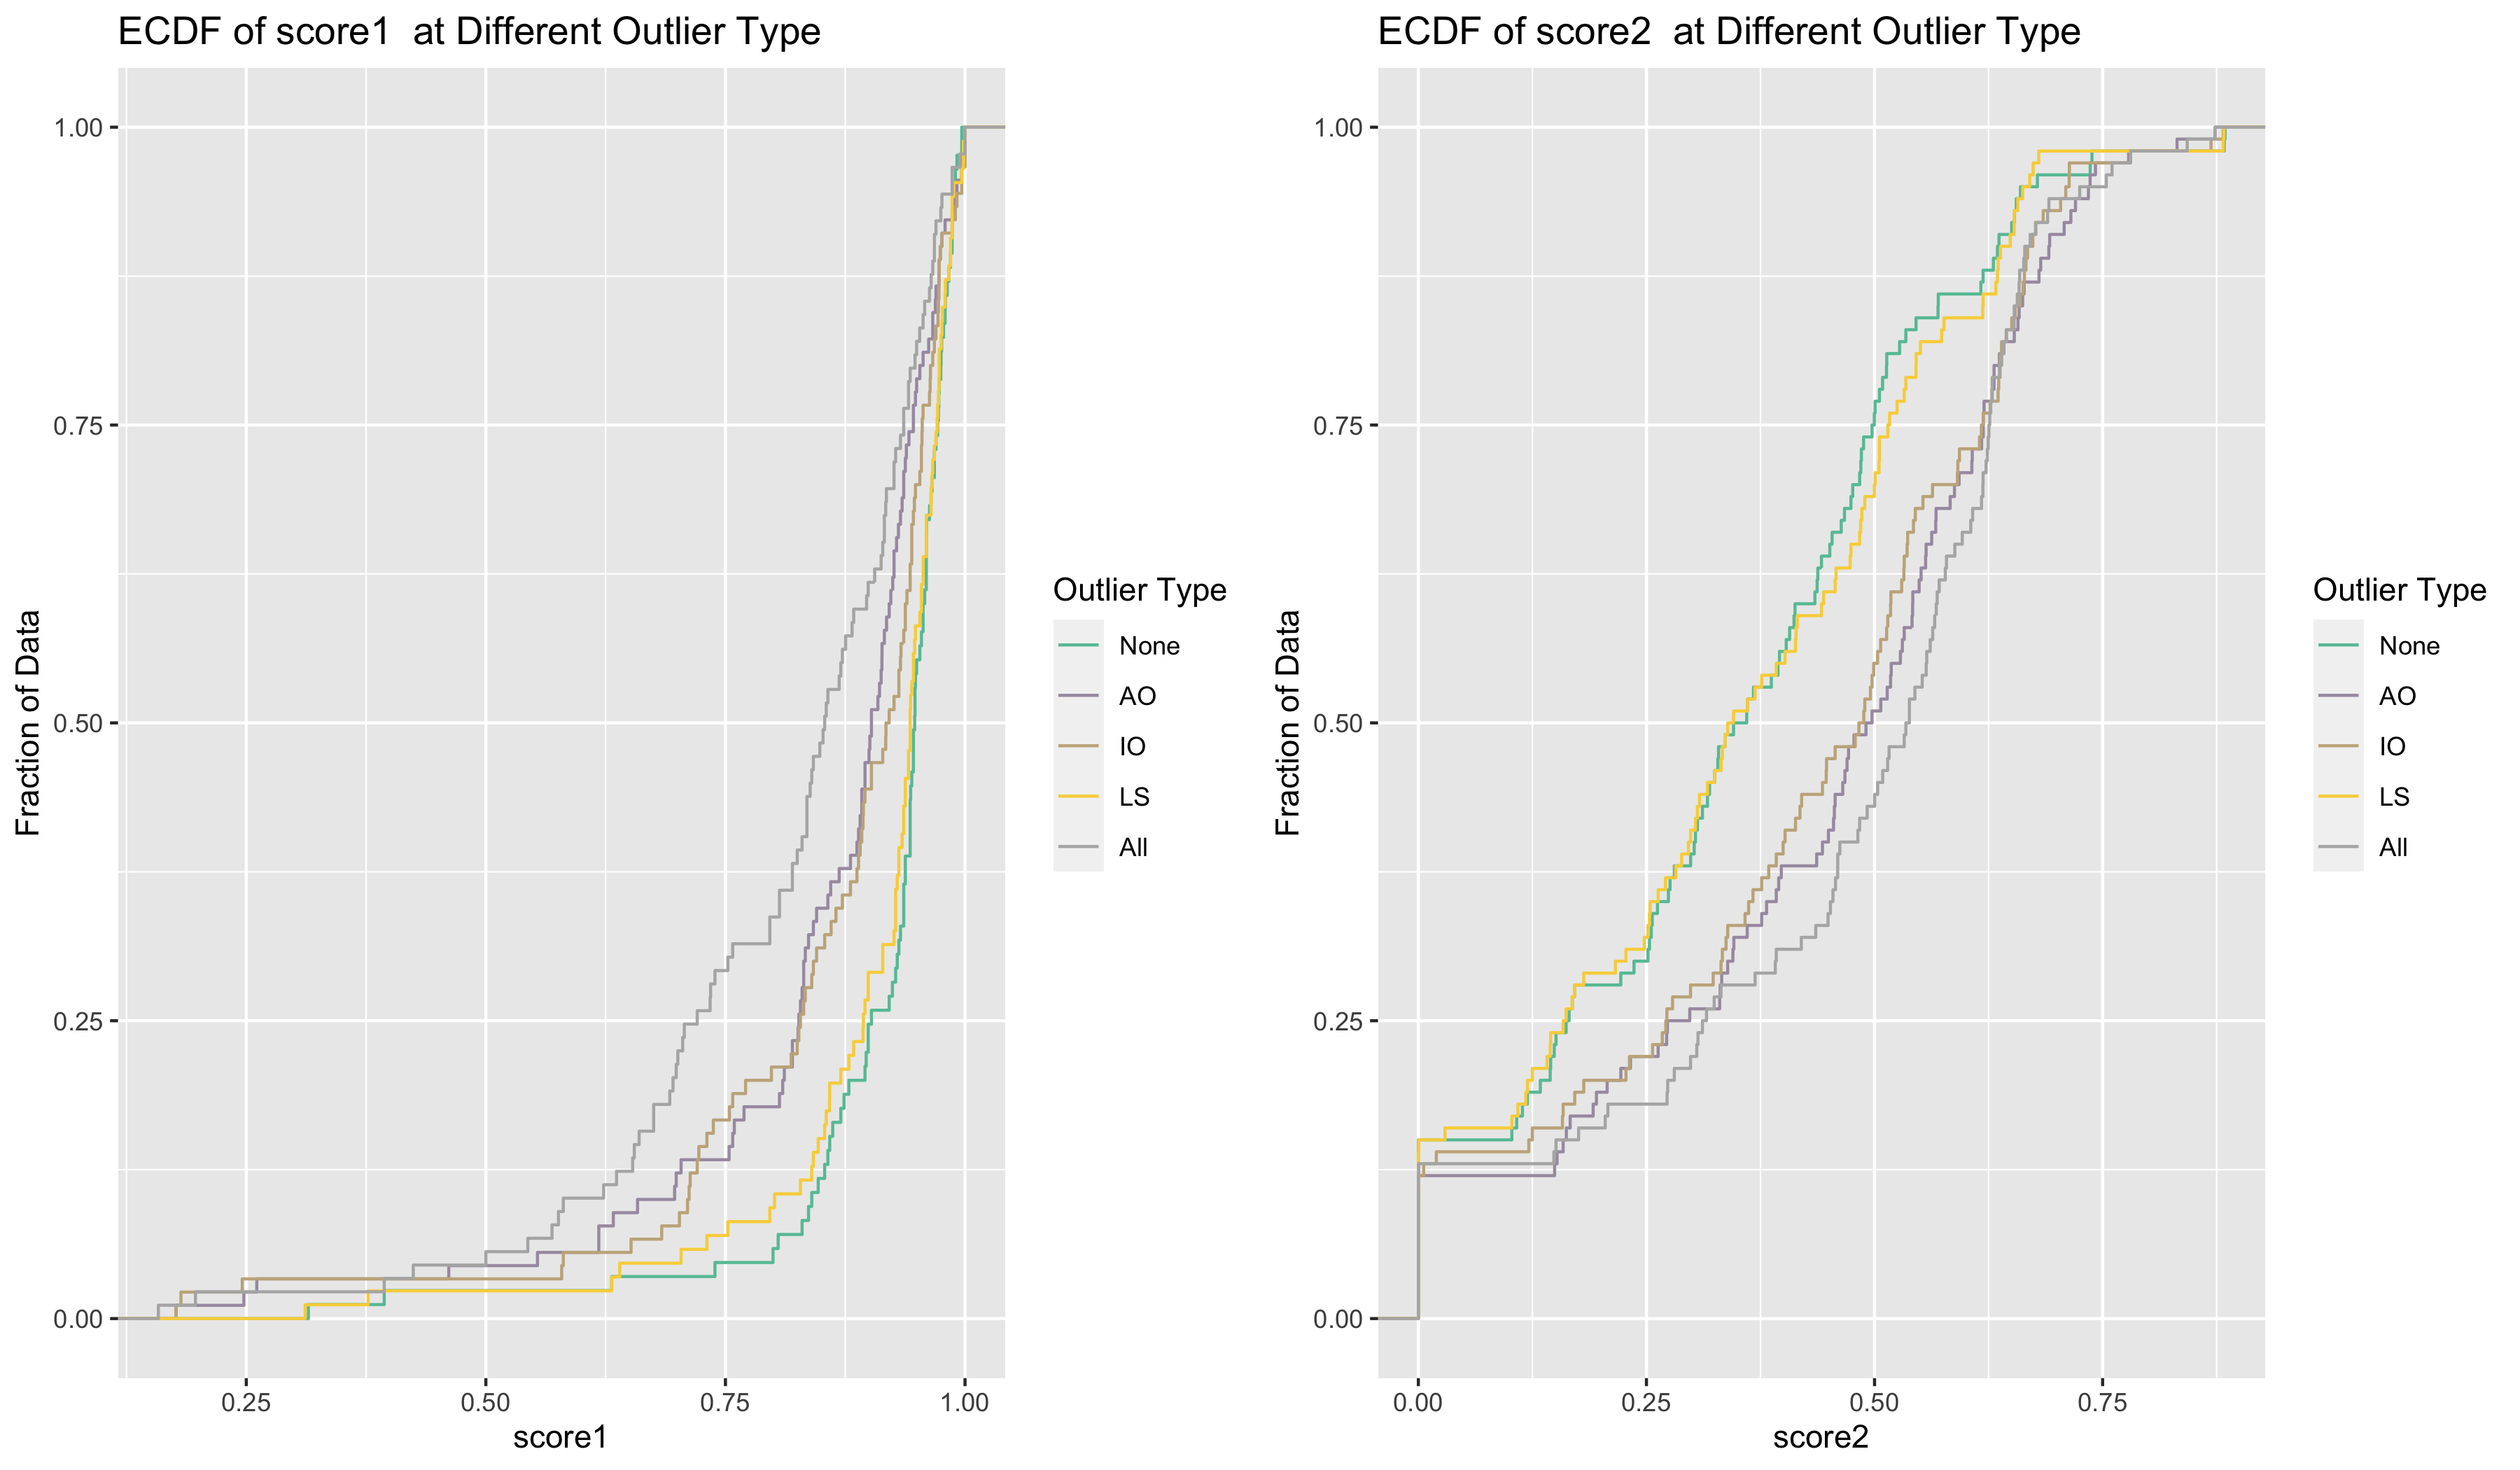
\includegraphics[width = 0.8\textwidth]{images/ECDFofscoresatDifferentOutlierTypeOfAR1,840,1,3.png}
\label{fig:fig1.3.4}
\end{figure}

\begin{table}[htbp]
  \begin{center}
    \caption{Configuration and Result of AR1 Model with Different Outlier Detections}
    \label{tab:tab1.3.4}
    \begin{tabular}{l|*{4}{c}}
      \textbf{outlier type} & \textbf{score 1} & \textbf{score 1 weight} & \textbf{score 2} & \textbf{score 2 weight} \\
      \hline
      None & 0.9168 & 48124 & 0.3463 & 59249\\
      AO & 0.8476 & 50288 & 0.4408 & 59249\\
      IO & 0.8567 & 49833 & 0.4237 & 59249\\
      LS & 0.9054 & 48360 & 0.3495 & 59249\\
      All & 0.8089 & 50807 & 0.4600 & 59249\\
    \end{tabular}
  \end{center}
\end{table}

\begin{figure}[htbp]
\caption{ECDF of Scores for Different Markov Models}
\centering
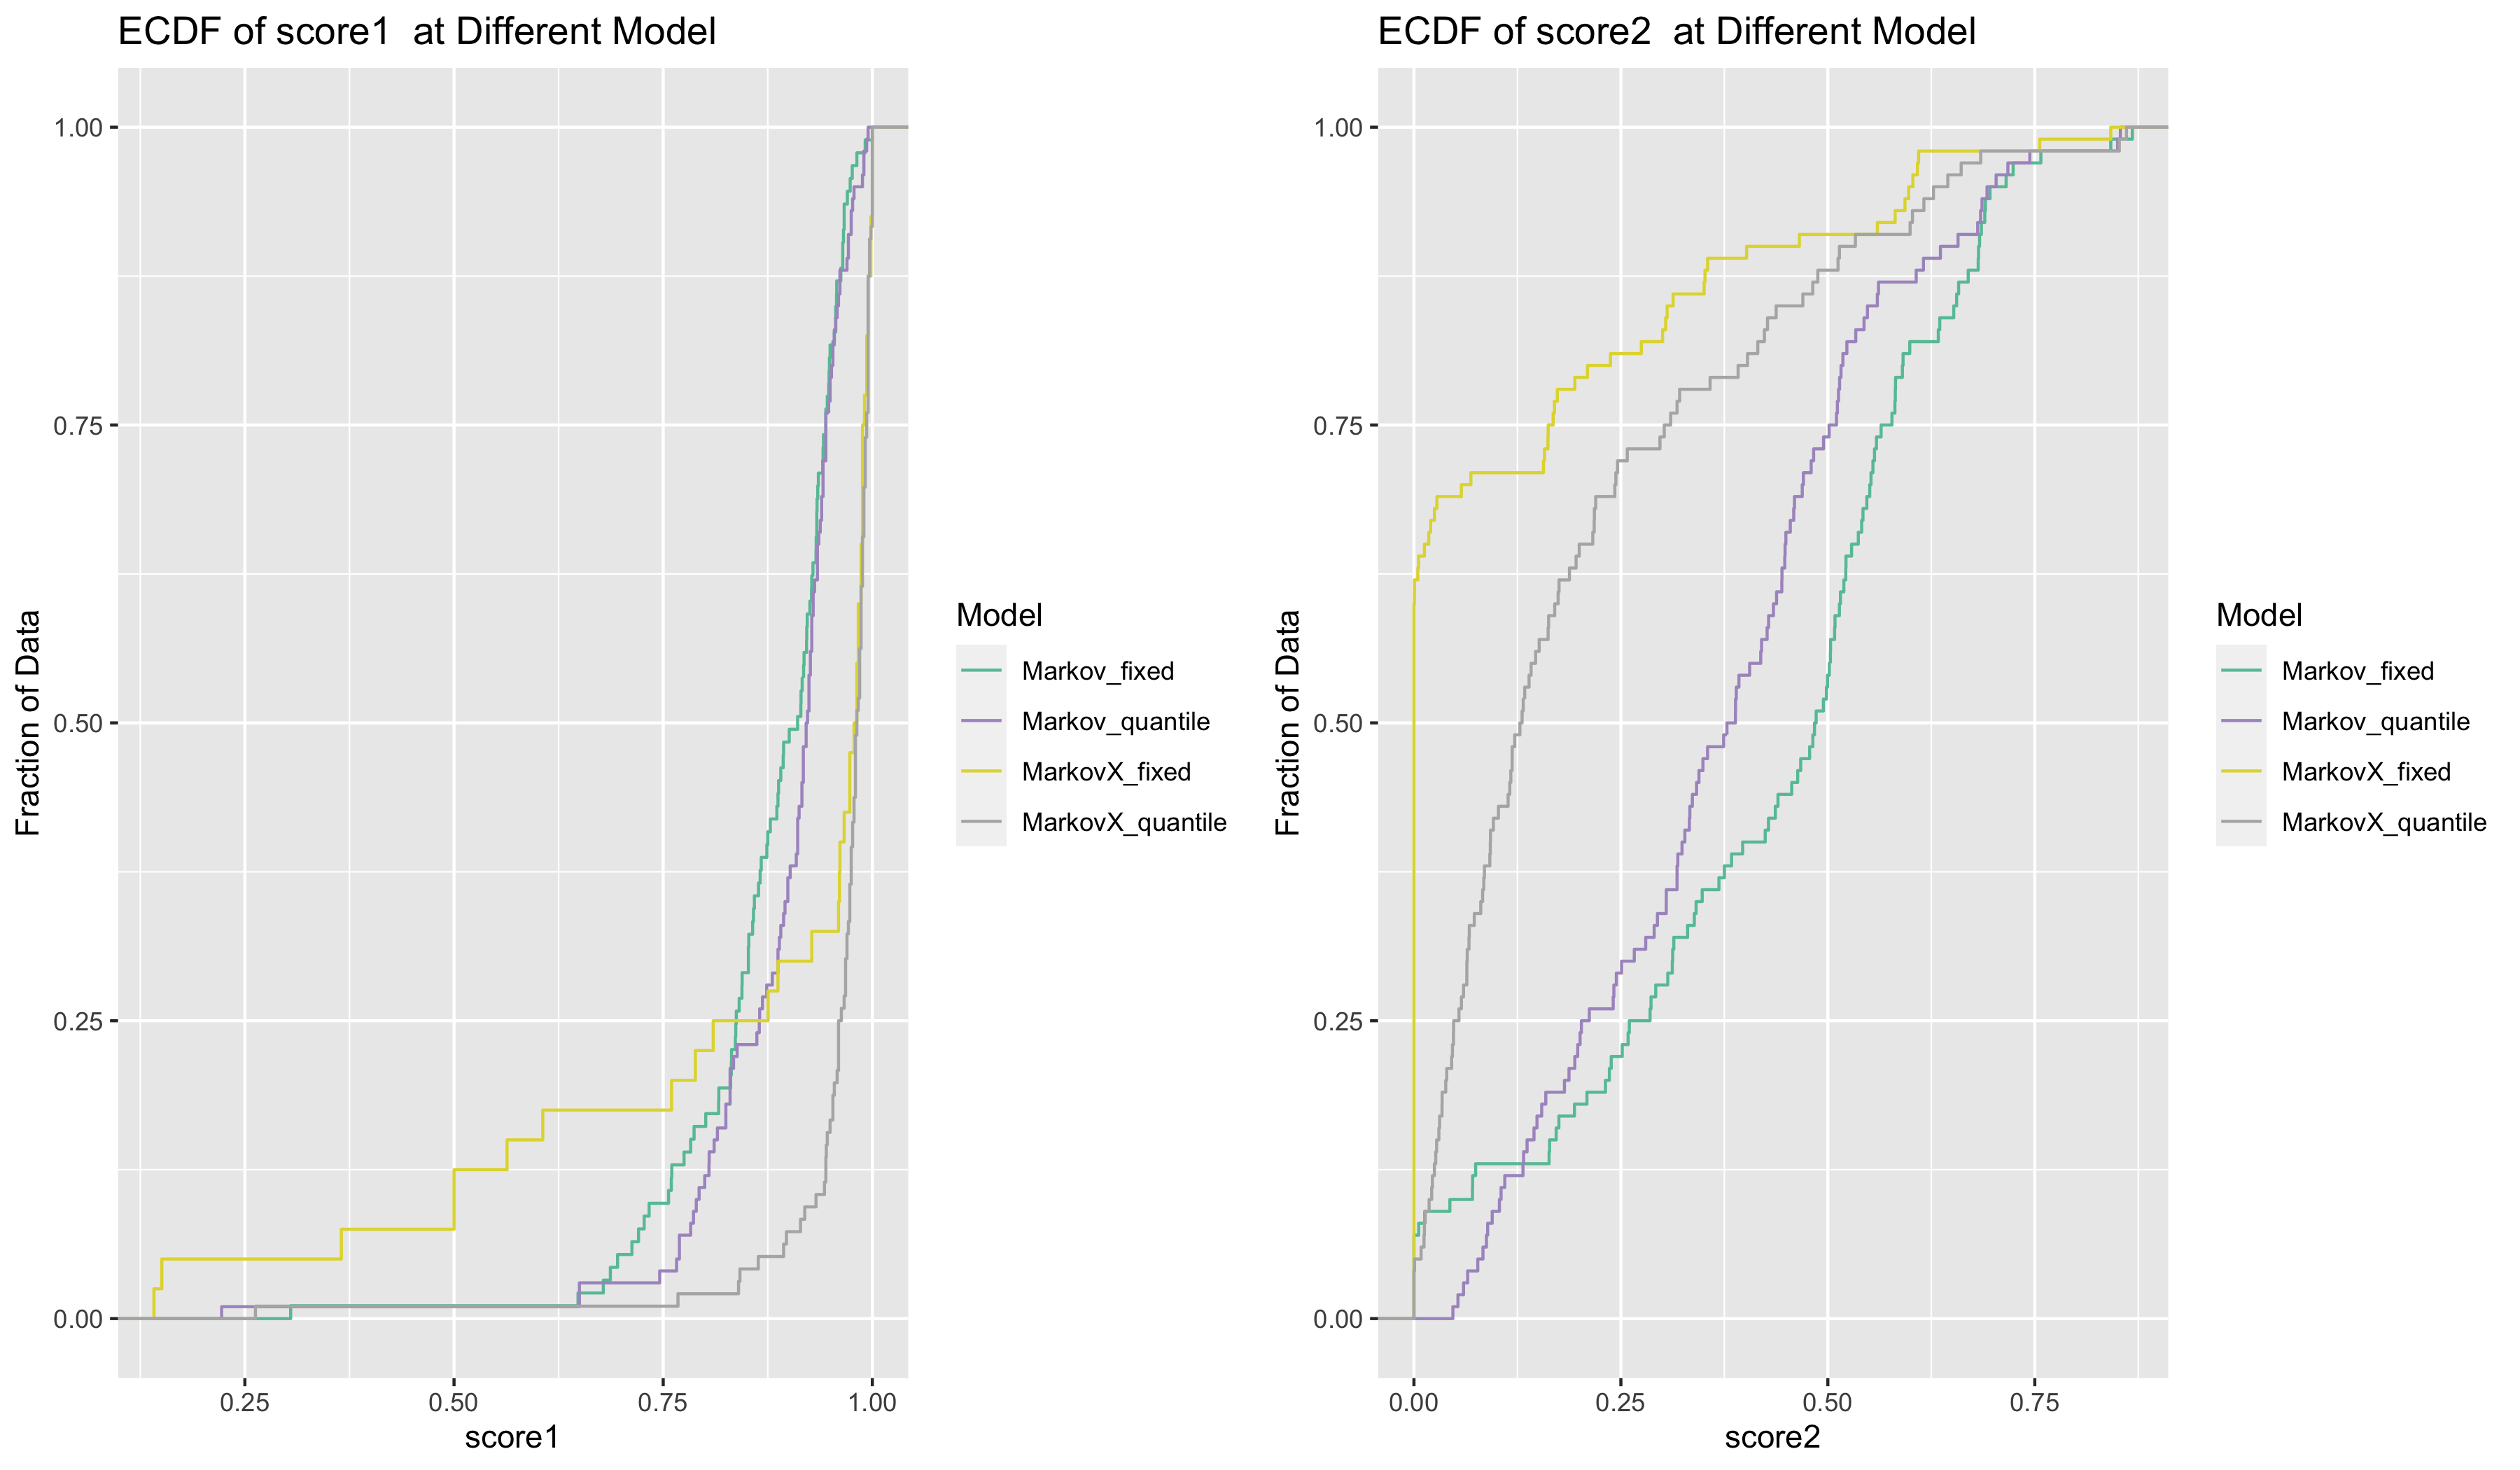
\includegraphics[width = 0.8\textwidth]{images/ECDFofscoresatDifferentModelOfMarkov_fixed,Markov_quantile,MarkovX_fixed,MarkovX_quantile.png}
\label{fig:fig1.3.5}
\end{figure}

\begin{table}[htbp]
  \begin{center}
    \caption{Configuration and Result of Markov Models with Different Partitioning Methods}
    \label{tab:tab1.3.5}
    \begin{tabular}{l|l|*{4}{c}}
      \textbf{model name} & \textbf{model name} & \textbf{score 1} & \textbf{score 1 weight} & \textbf{score 2} & \textbf{score 2 weight} \\
      \hline
      Markov & fixed & 0.8792 & 45459 & 0.4231 & 59249\\
      MarkovX & fixed & 0.9365 & 17384 & 0.1123 & 59249\\
      Markov & quantile & 0.8945 & 57589 & 0.3741 & 59249\\
      MarkovX & quantile & 0.9634 & 56648 & 0.2066 & 59249\\
    \end{tabular}
  \end{center}
\end{table}

\begin{figure}[htbp]
\caption{ECDF of Scores for Different States for Markov Models}
\centering
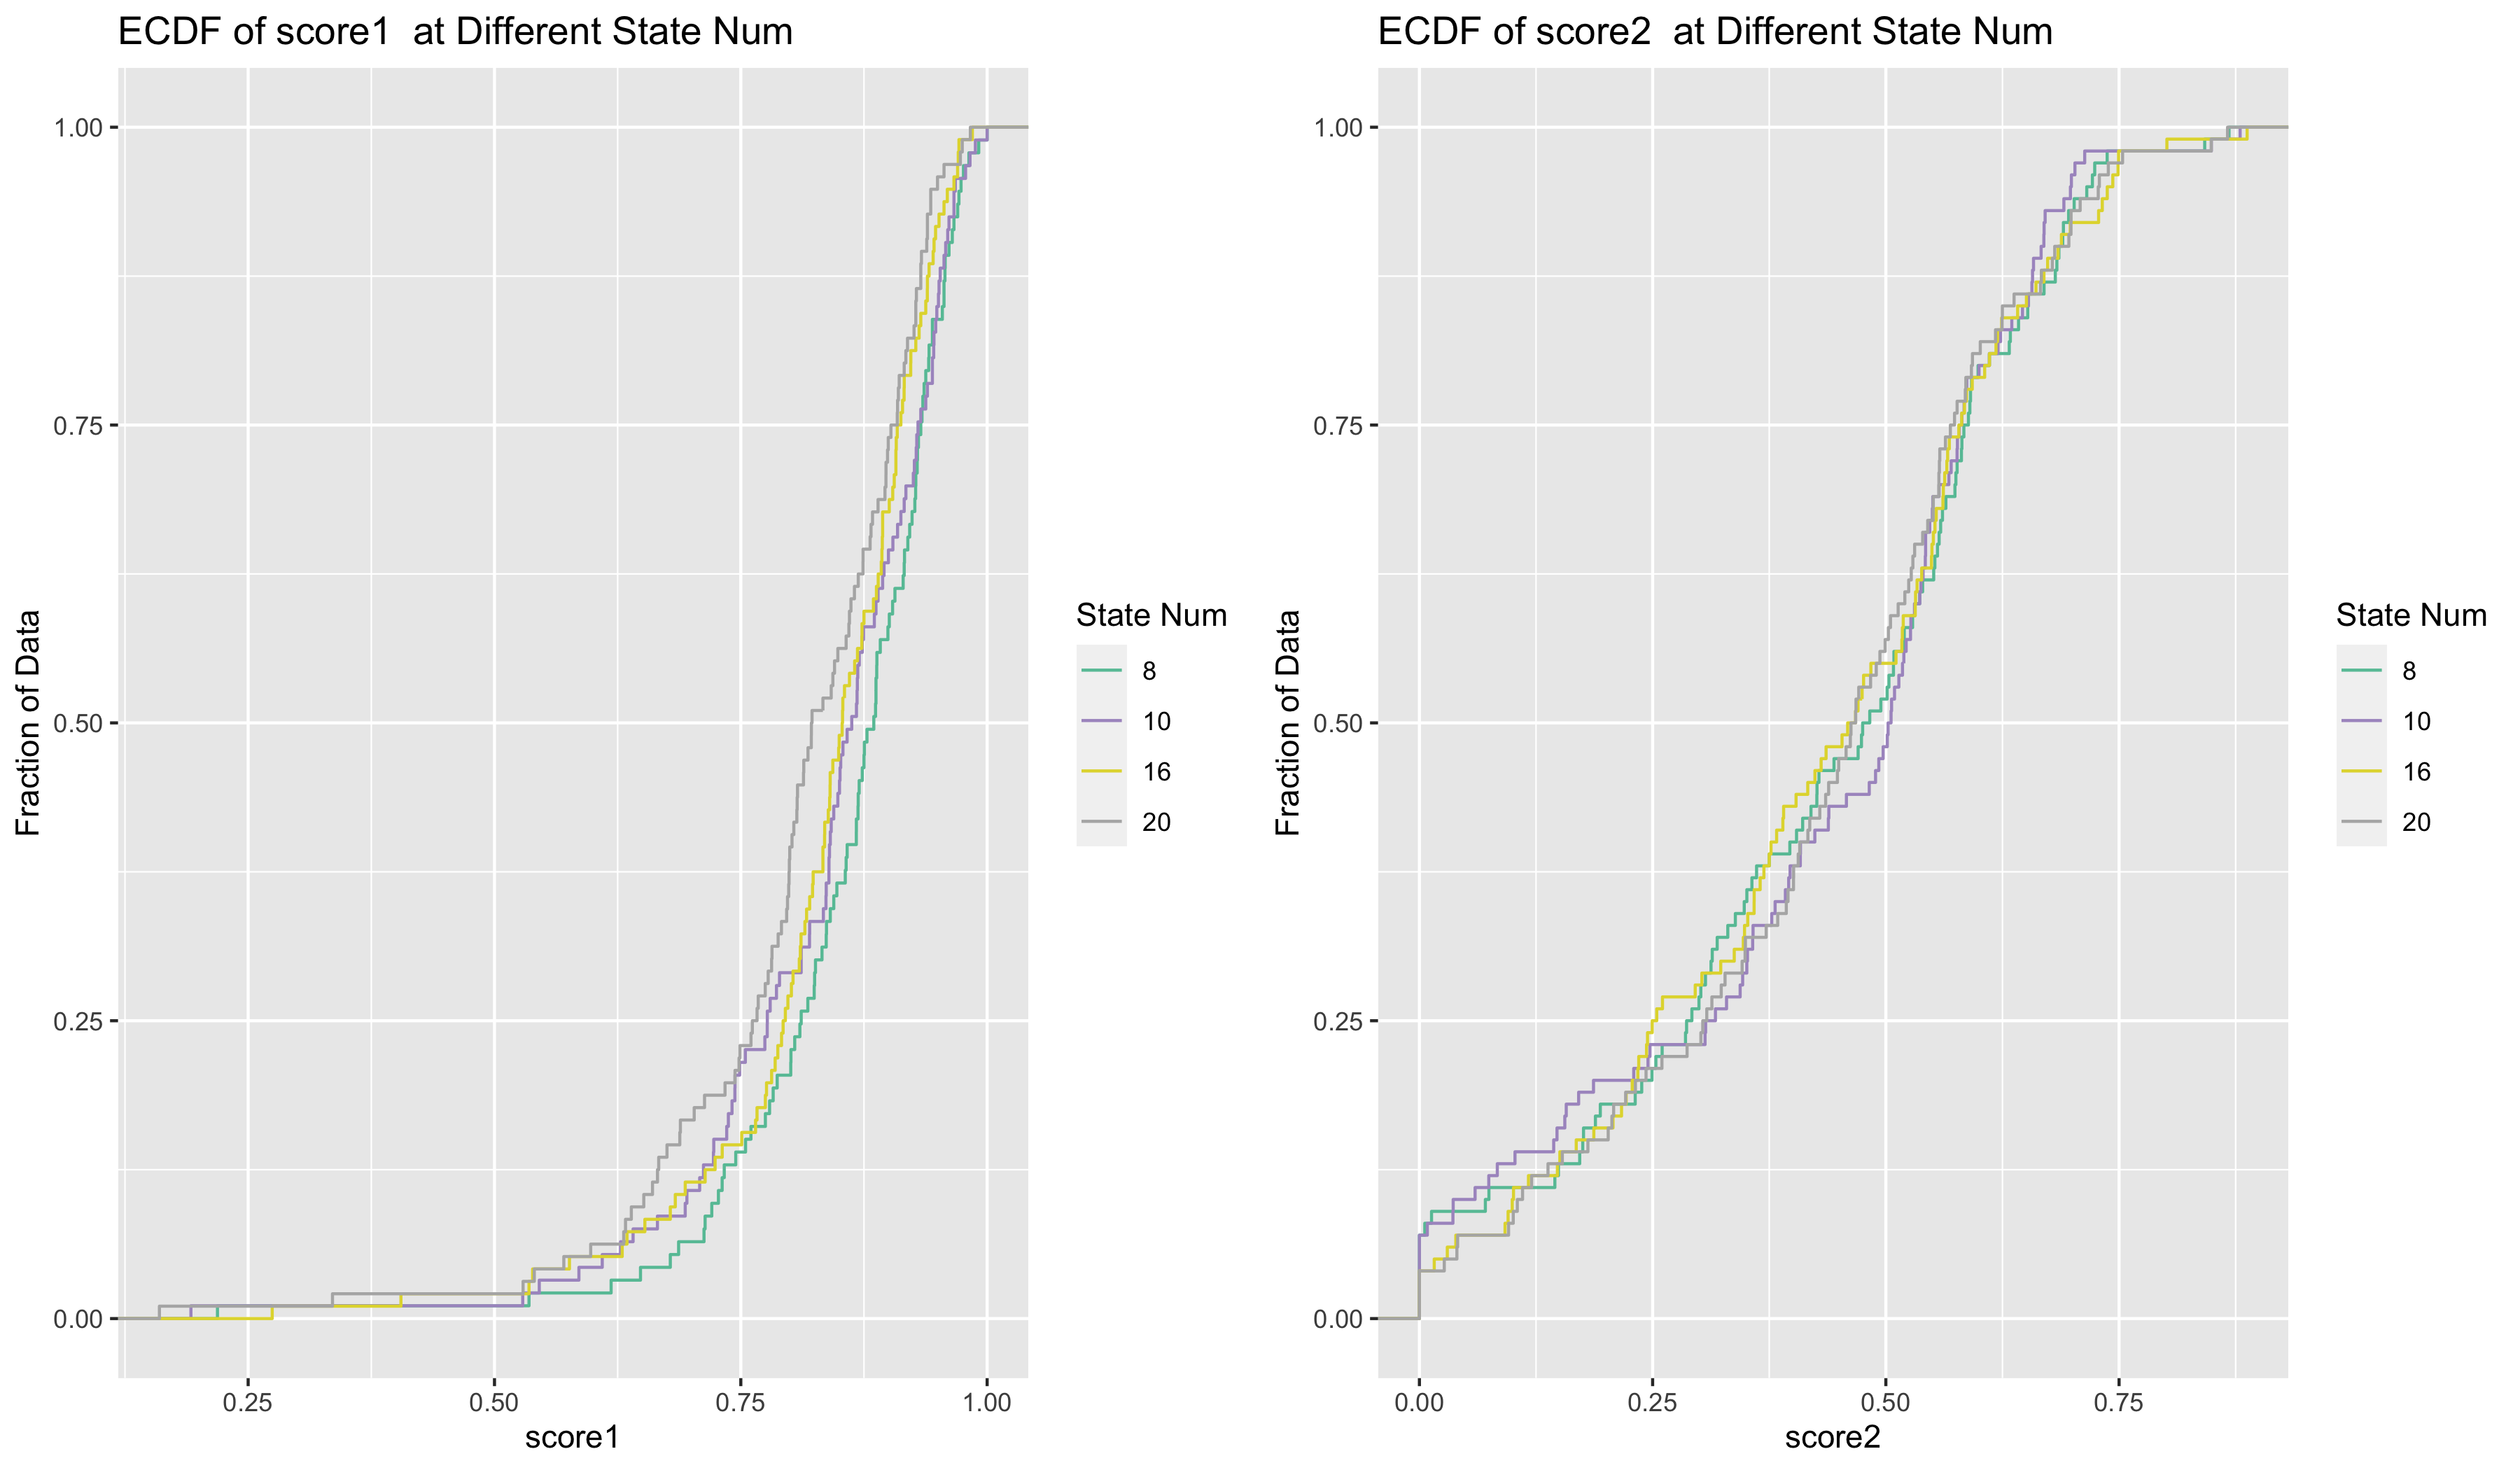
\includegraphics[width = 0.8\textwidth]{images/ECDFofscoresatDifferentStateNumOfMarkov,840,3,1.png}
\label{fig:fig1.3.6}
\end{figure}

\begin{table}[htbp]
  \begin{center}
    \caption{Configuration and Result of Markov Model with Different Number of States}
    \label{tab:tab1.3.6}
    \begin{tabular}{l|*{4}{c}}
      \textbf{state num} & \textbf{score 1} & \textbf{score 1 weight} & \textbf{score 2} & \textbf{score 2 weight} \\
      \hline
      8 & 0.8618 & 46053 & 0.4306 & 59249\\
      10 & 0.8396 & 46253 & 0.4311 & 59249\\
      16 & 0.8379 & 46658 & 0.4282 & 59249\\
      20 & 0.8139 & 48282 & 0.4339 & 59249\\
    \end{tabular}
  \end{center}
\end{table}

\begin{figure}[htbp]
\caption{ECDF of Scores for Different Multivariate Models}
\centering
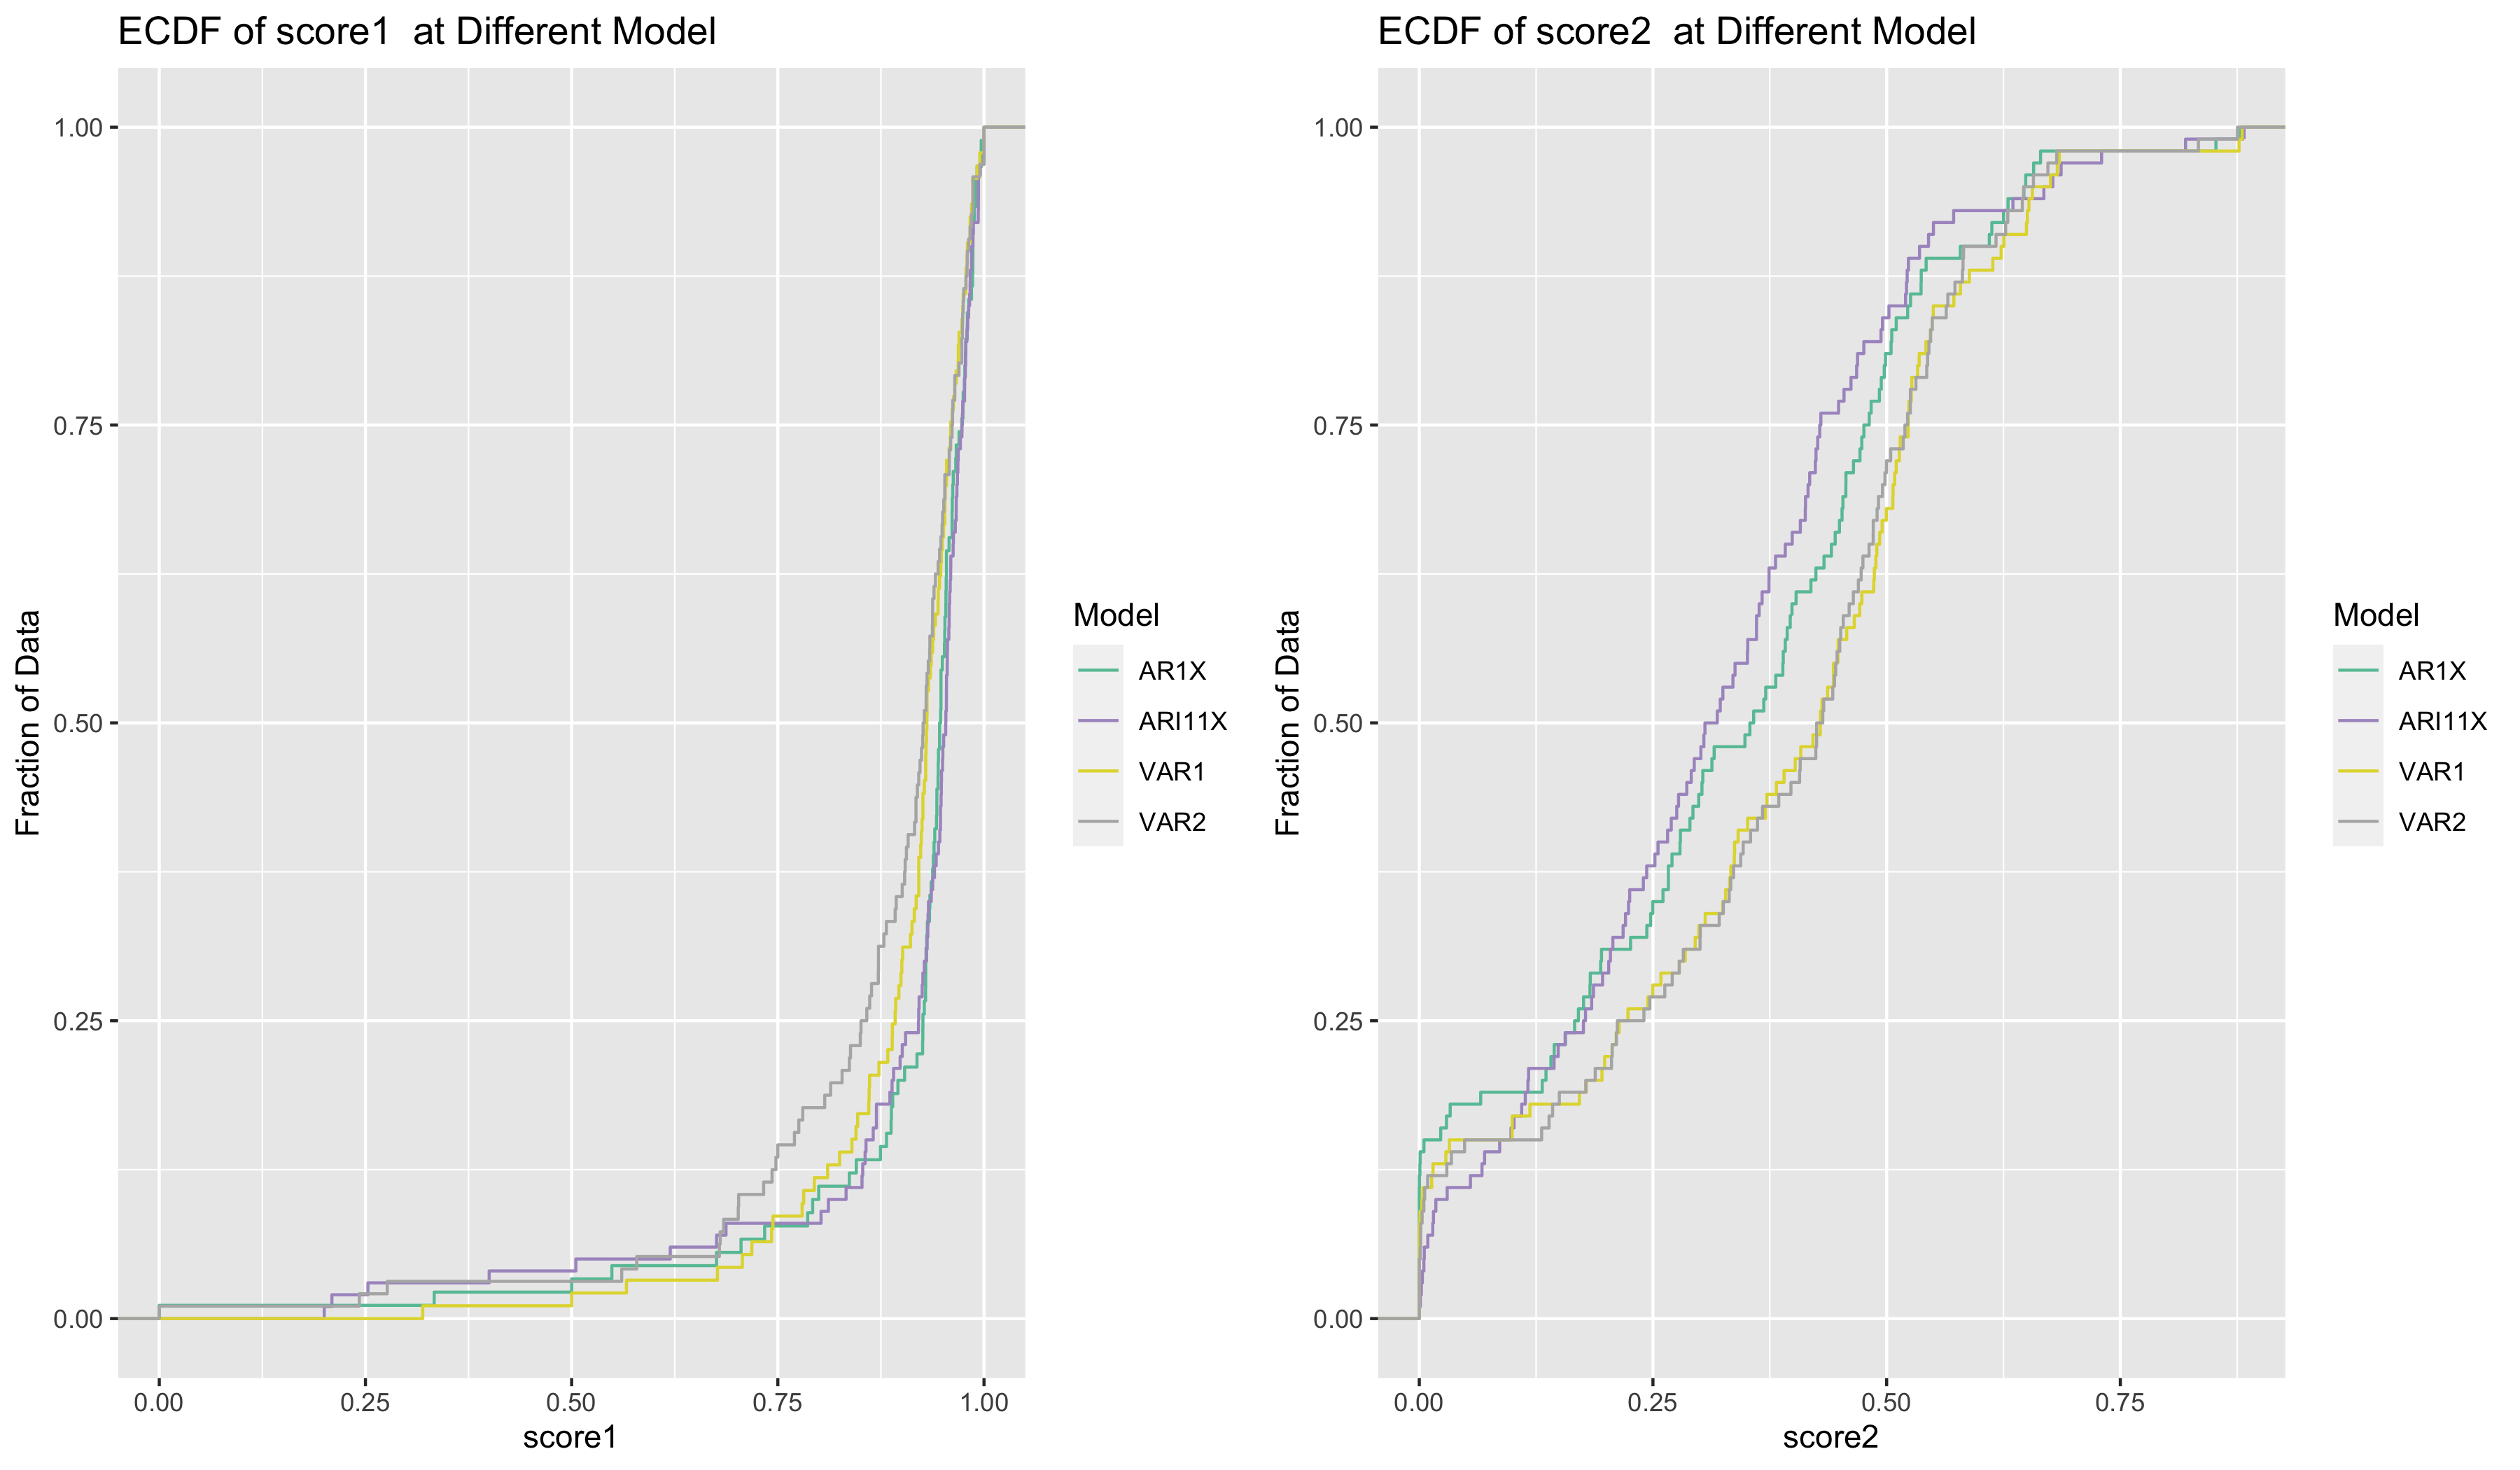
\includegraphics[width = 0.8\textwidth]{images/ECDFofscoresatDifferentModelOfAR1X,ARI11X,VAR1,VAR2.png}
\label{fig:fig1.3.7}
\end{figure}

\begin{table}[htbp]
  \begin{center}
    \caption{Configuration and Result of AR1 Model with Different Outlier Detections}
    \label{tab:tab1.3.7}
    \begin{tabular}{l|*{4}{c}}
      \textbf{model name} & \textbf{score 1} & \textbf{score 1 weight} & \textbf{score 2} & \textbf{score 2 weight} \\
      \hline
      AR1X & 0.9293 & 45094 & 0.3270 & 59249\\
      ARI11X & 0.9238 & 45778 & 0.3140 & 59249\\
      VAR1 & 0.9102 & 47837 & 0.3750 & 59249\\
      VAR2 & 0.8910 & 48459 & 0.3742 & 59249\\
    \end{tabular}
  \end{center}
\end{table}

\subsubsection{Aggregation VS Extrapolation}
Ref to Section 1.4, include Fig \ref{fig:fig1.4.1} and Table \ref{tab:tab1.4.1}.

\begin{figure}[htbp]
\caption{ECDF of Scores for Different Extrapolation Steps}
\centering
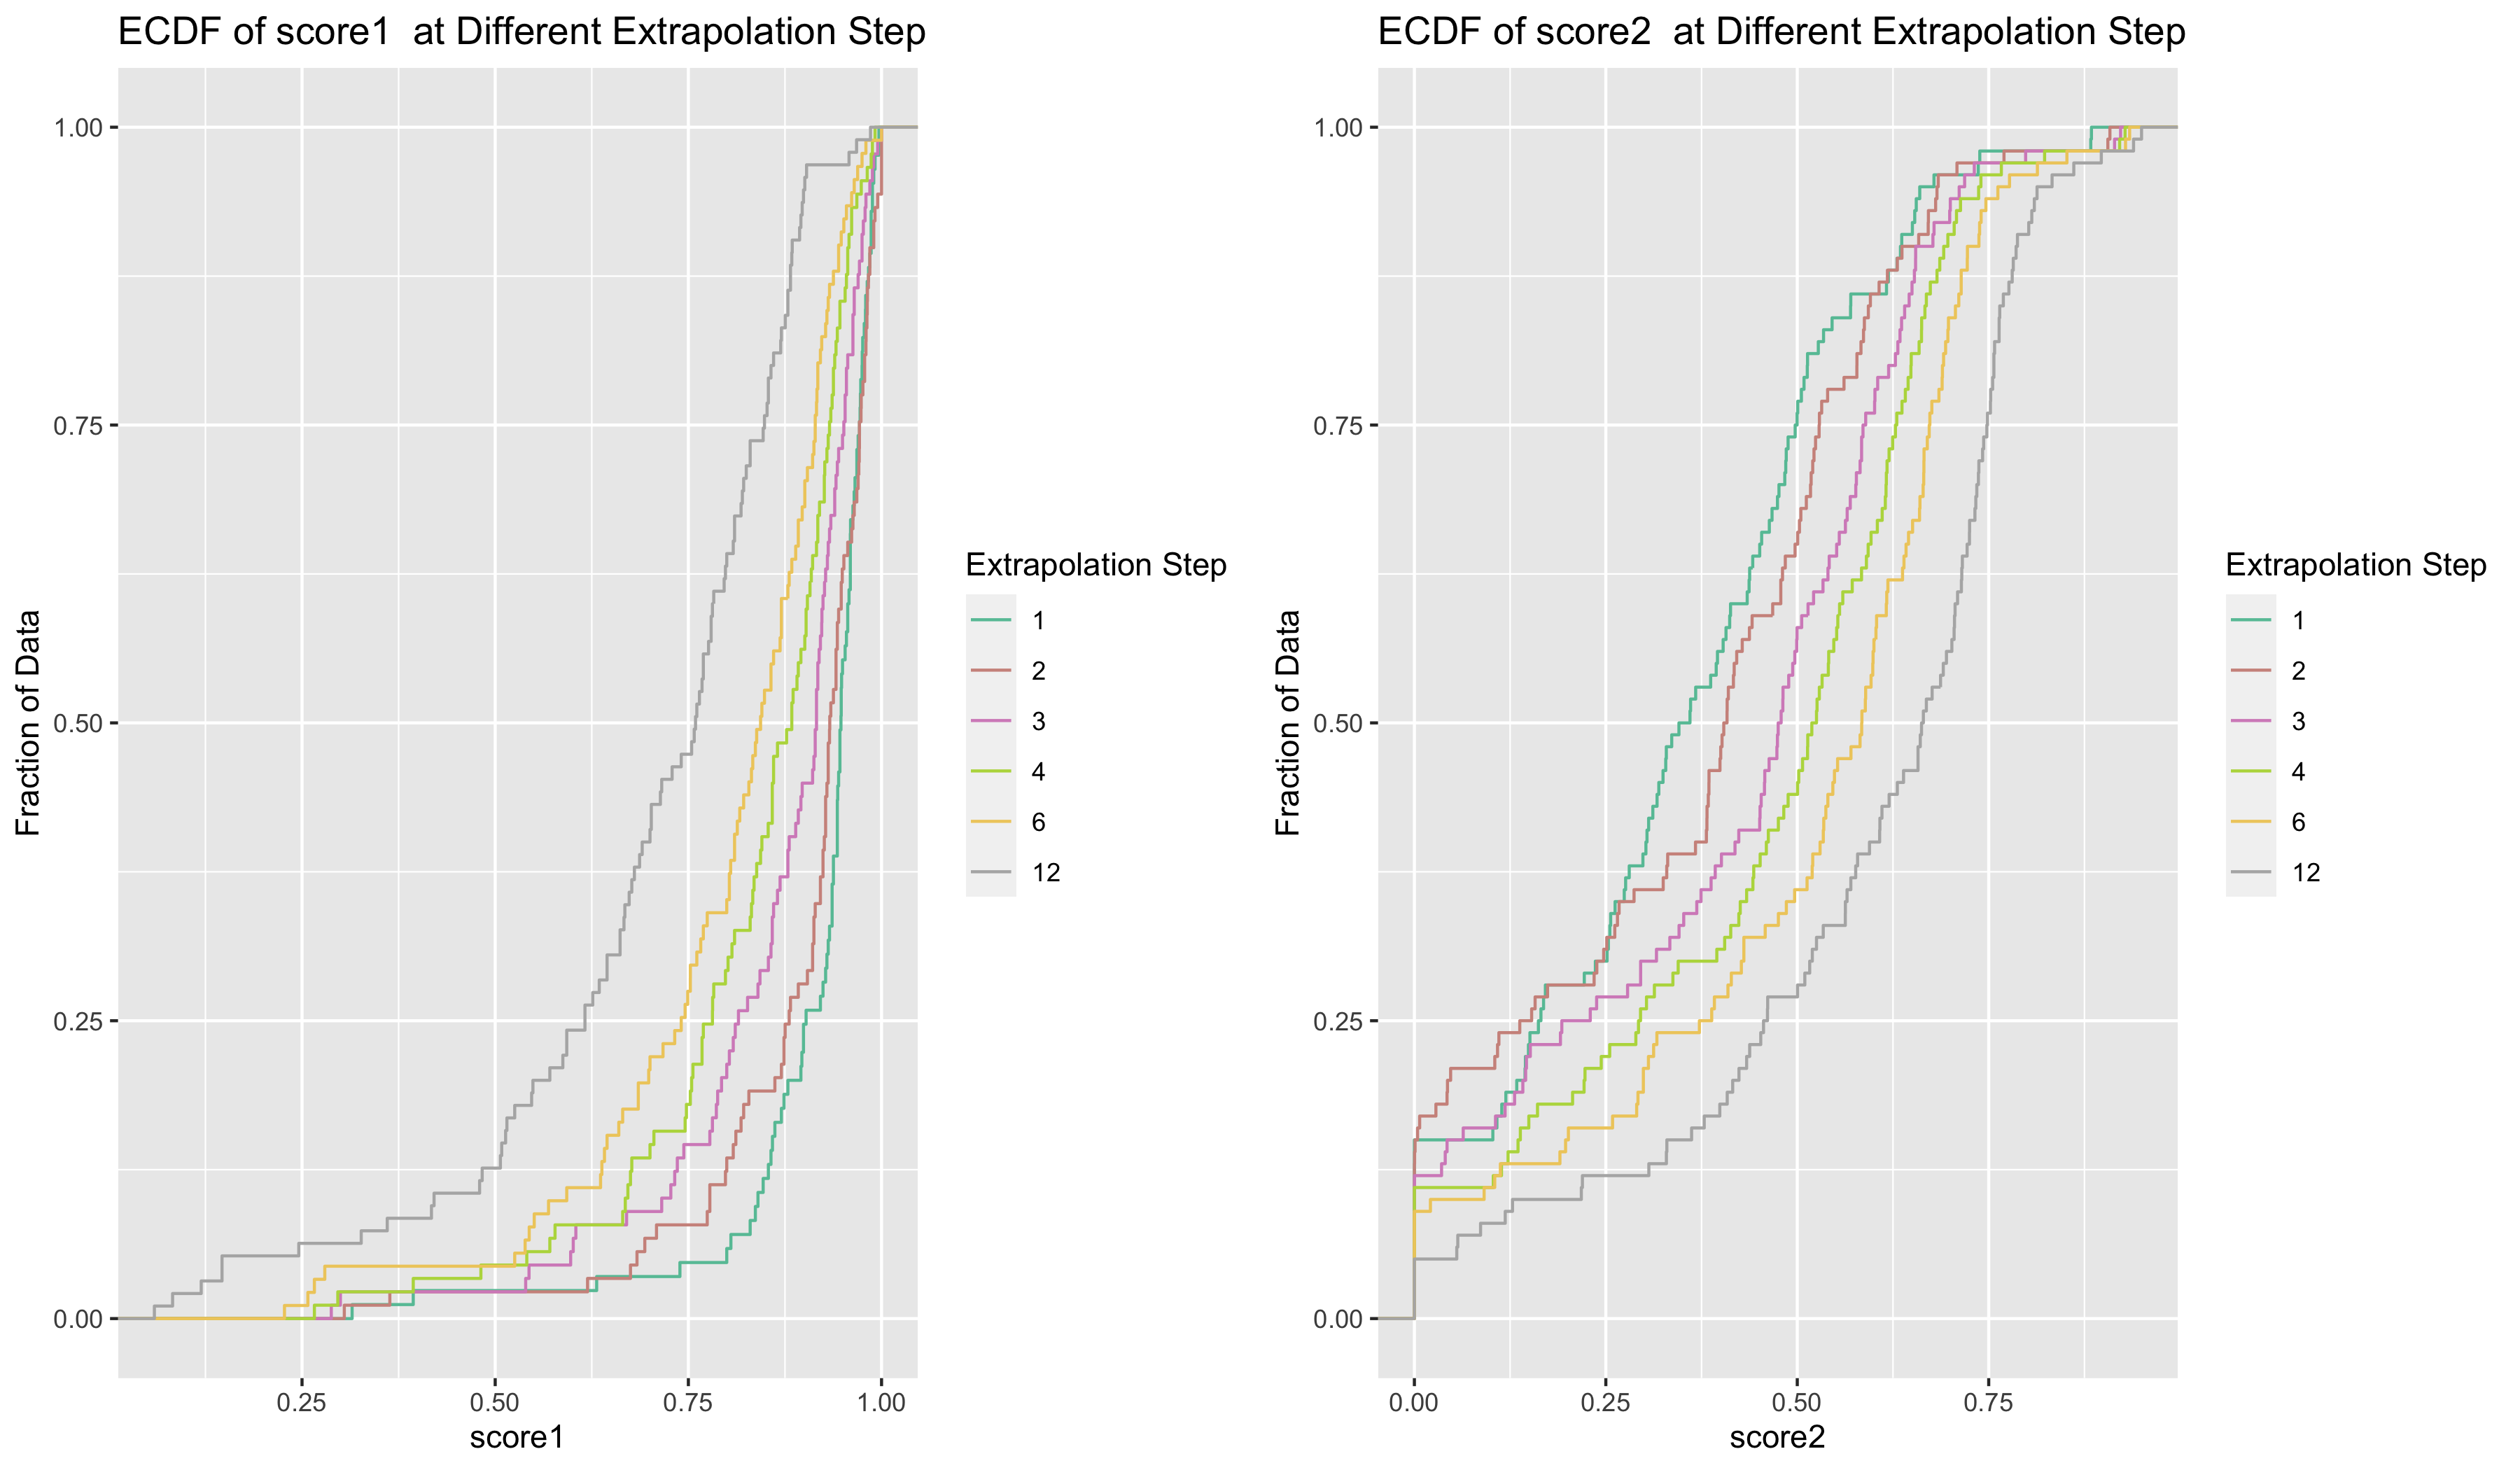
\includegraphics[width = 0.8\textwidth]{images/ECDFofscoresatDifferentExtrapolationStepOfAR1,840,1,3.png}
\label{fig:fig1.4.1}
\end{figure}

\begin{table}[htbp]
  \begin{center}
    \caption{Configuration and Result of AR1 Model with Different Extrapolation Steps}
    \label{tab:tab1.4.1}
    \begin{tabular}{l|l|*{4}{c}}
      \textbf{window size} & \textbf{extrap step} & \textbf{score 1} & \textbf{score 1 weight} & \textbf{score 2} & \textbf{score 2 weight} \\
      \hline
      12 & 1 & 0.9168 & 48124 & 0.3463 & 59249\\
      6 & 2 & 0.8923 & 47700 & 0.3642 & 59249\\
      4 & 3 & 0.8641 & 51370 & 0.4156 & 59249\\
      3 & 4 & 0.8354 & 52424 & 0.4569 & 59249\\
      2 & 6 & 0.7993 & 53626 & 0.5045 & 59249\\
      1 & 12 & 0.6953 & 56316 & 0.5833 & 59249\\
    \end{tabular}
  \end{center}
\end{table}

\subsubsection{Offline Training VS Online Training}
Ref to Section 1.5, include Fig \ref{fig:fig1.5.1}, Table \ref{tab:tab1.5.1}.

\begin{figure}
    \caption{ECDF of Scores for Different Training Policies}
    \centering
    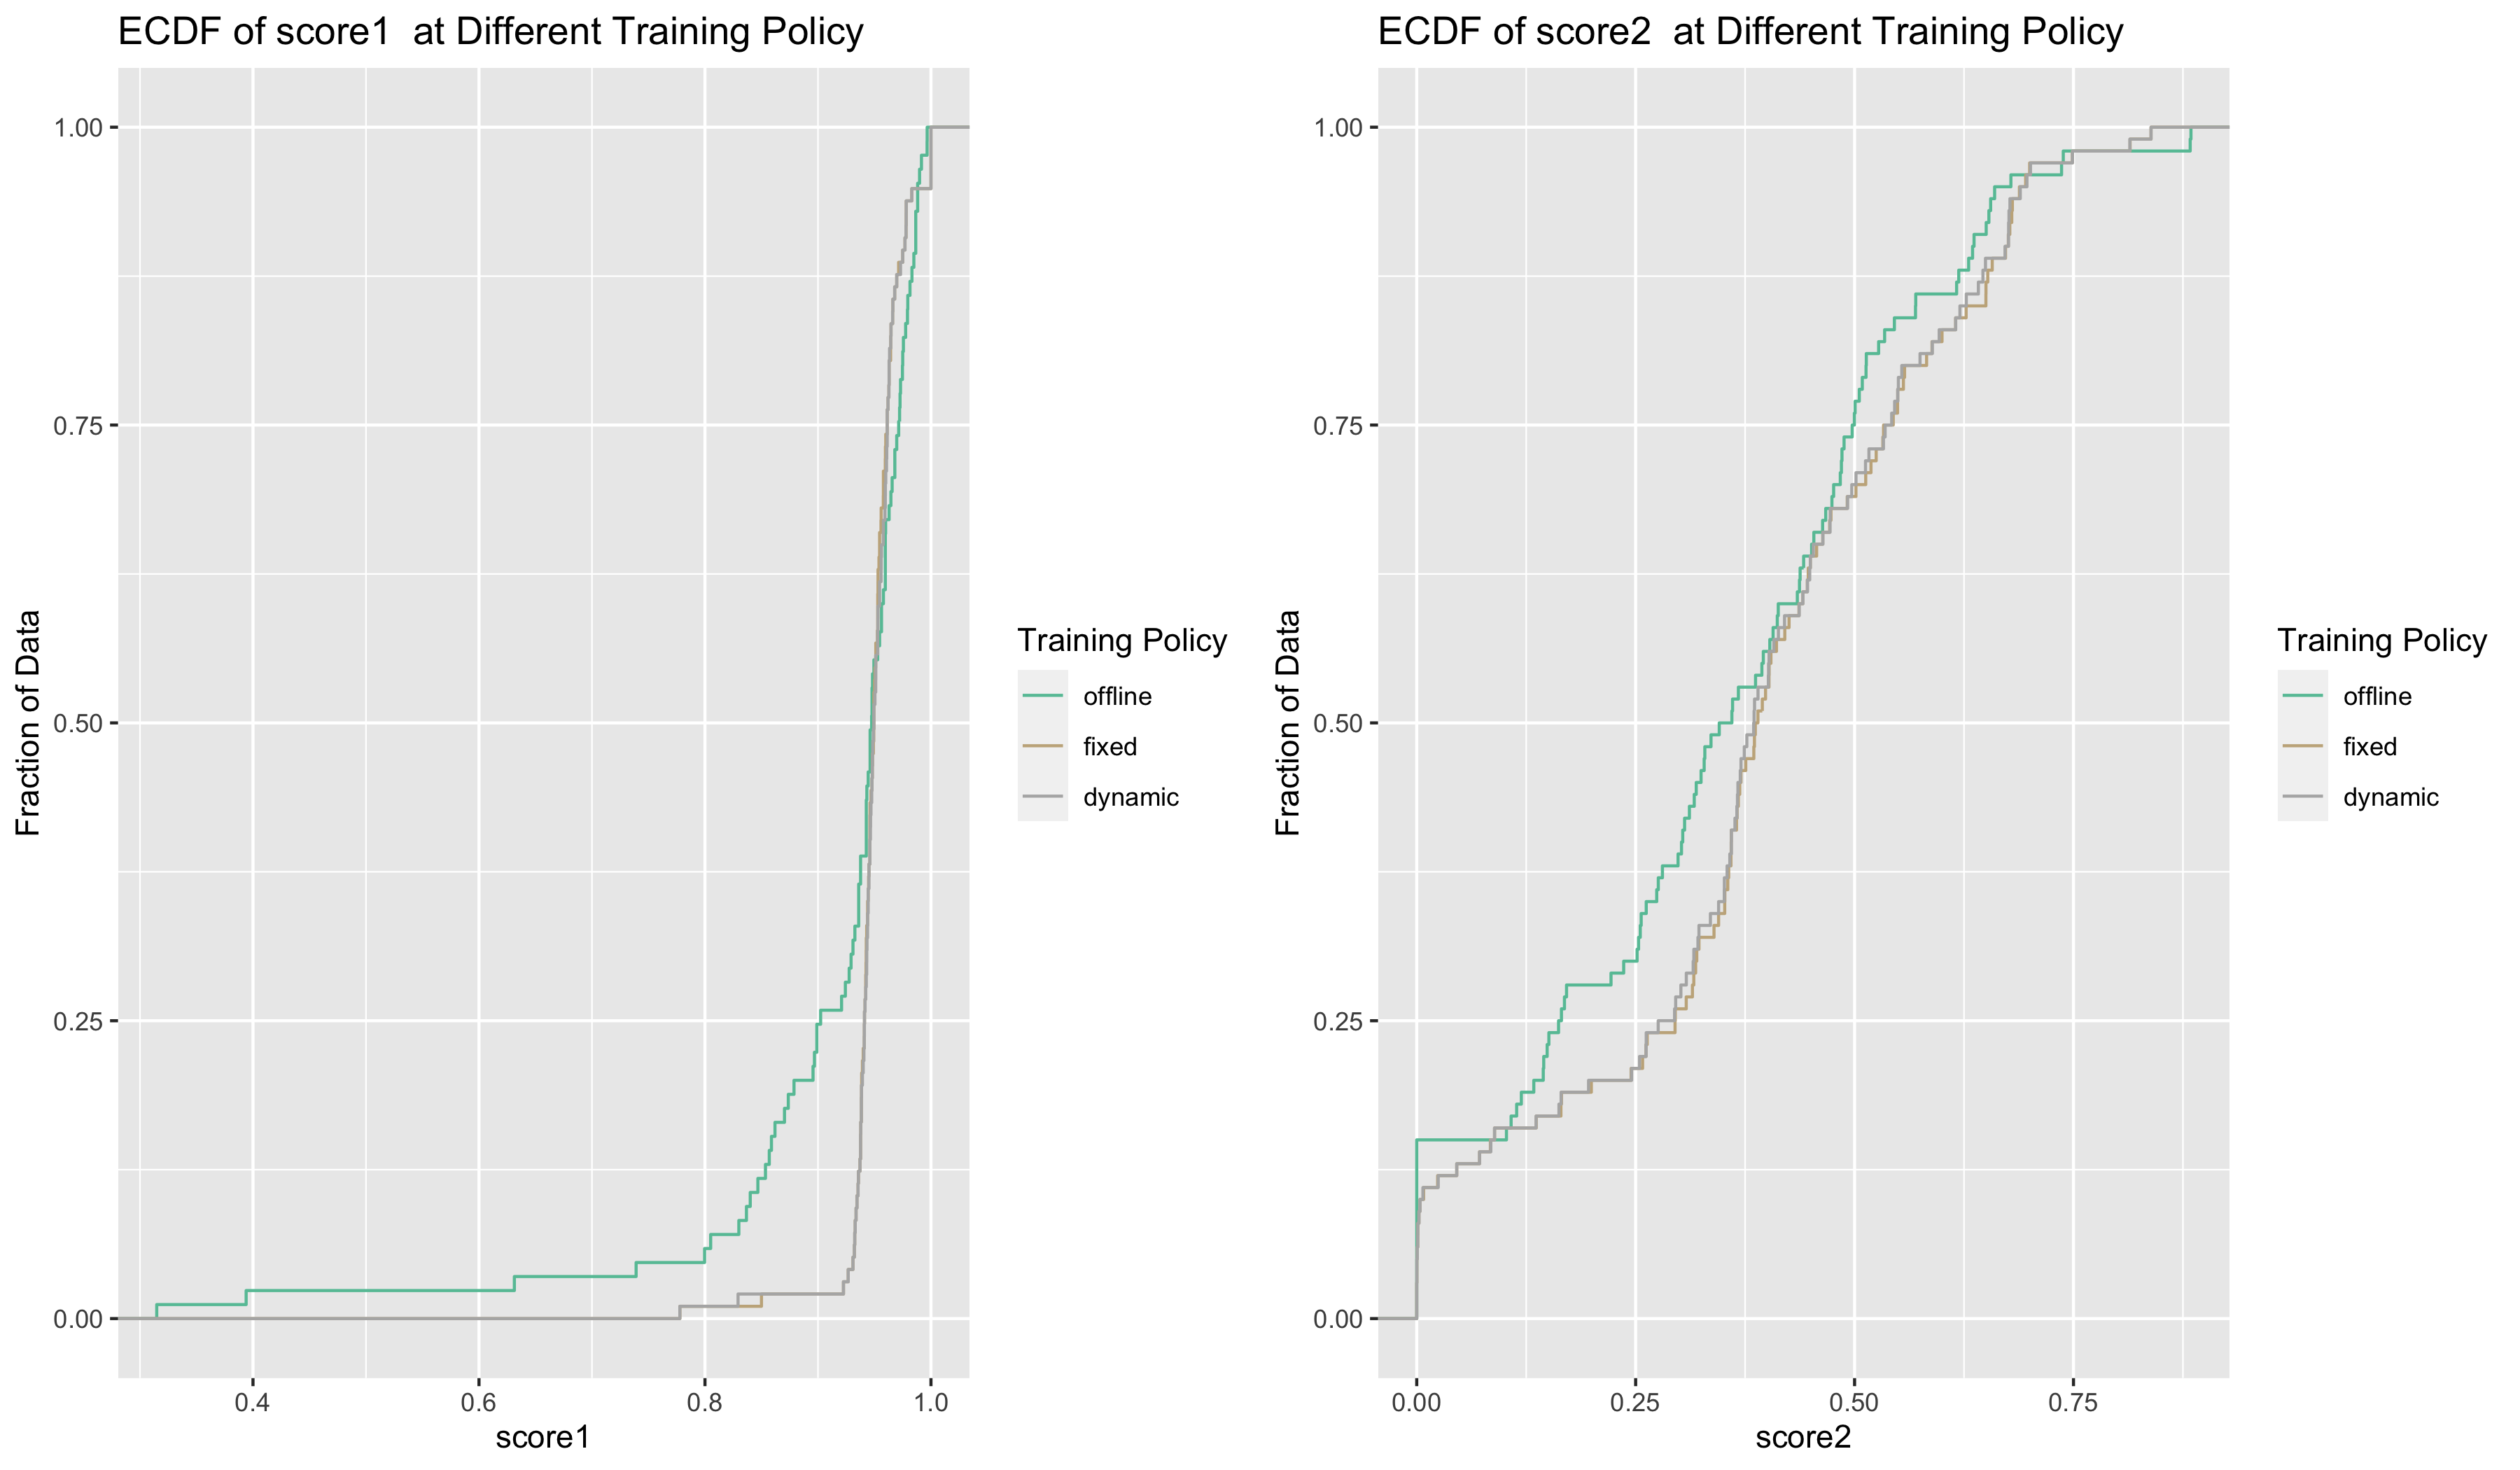
\includegraphics[width = 0.8\textwidth]{images/ECDFofscoresatDifferentTrainingPolicyOfAR1,840,1,3.png}
    \label{fig:fig1.5.1}
\end{figure}

\begin{table}[htbp]
  \begin{center}
    \caption{Configuration and Result of AR1 Model with Different Training Policies}
    \label{tab:tab1.5.1}
    \begin{tabular}{l|*{4}{c}}
      \textbf{training policy} & \textbf{score 1} & \textbf{score 1 weight} & \textbf{score 2} & \textbf{score 2 weight} \\
      \hline
      offline & 0.9168 & 48124 & 0.3463 & 59249\\
      fixed & 0.9504 & 47518 & 0.3873 & 59249\\
      dynamic & 0.9508 & 47422 & 0.3844 & 59249\\
    \end{tabular}
  \end{center}
\end{table}

\begin{figure}
    \caption{ECDF of Scores for Different Batch Size of Dynamic Training}
    \centering
    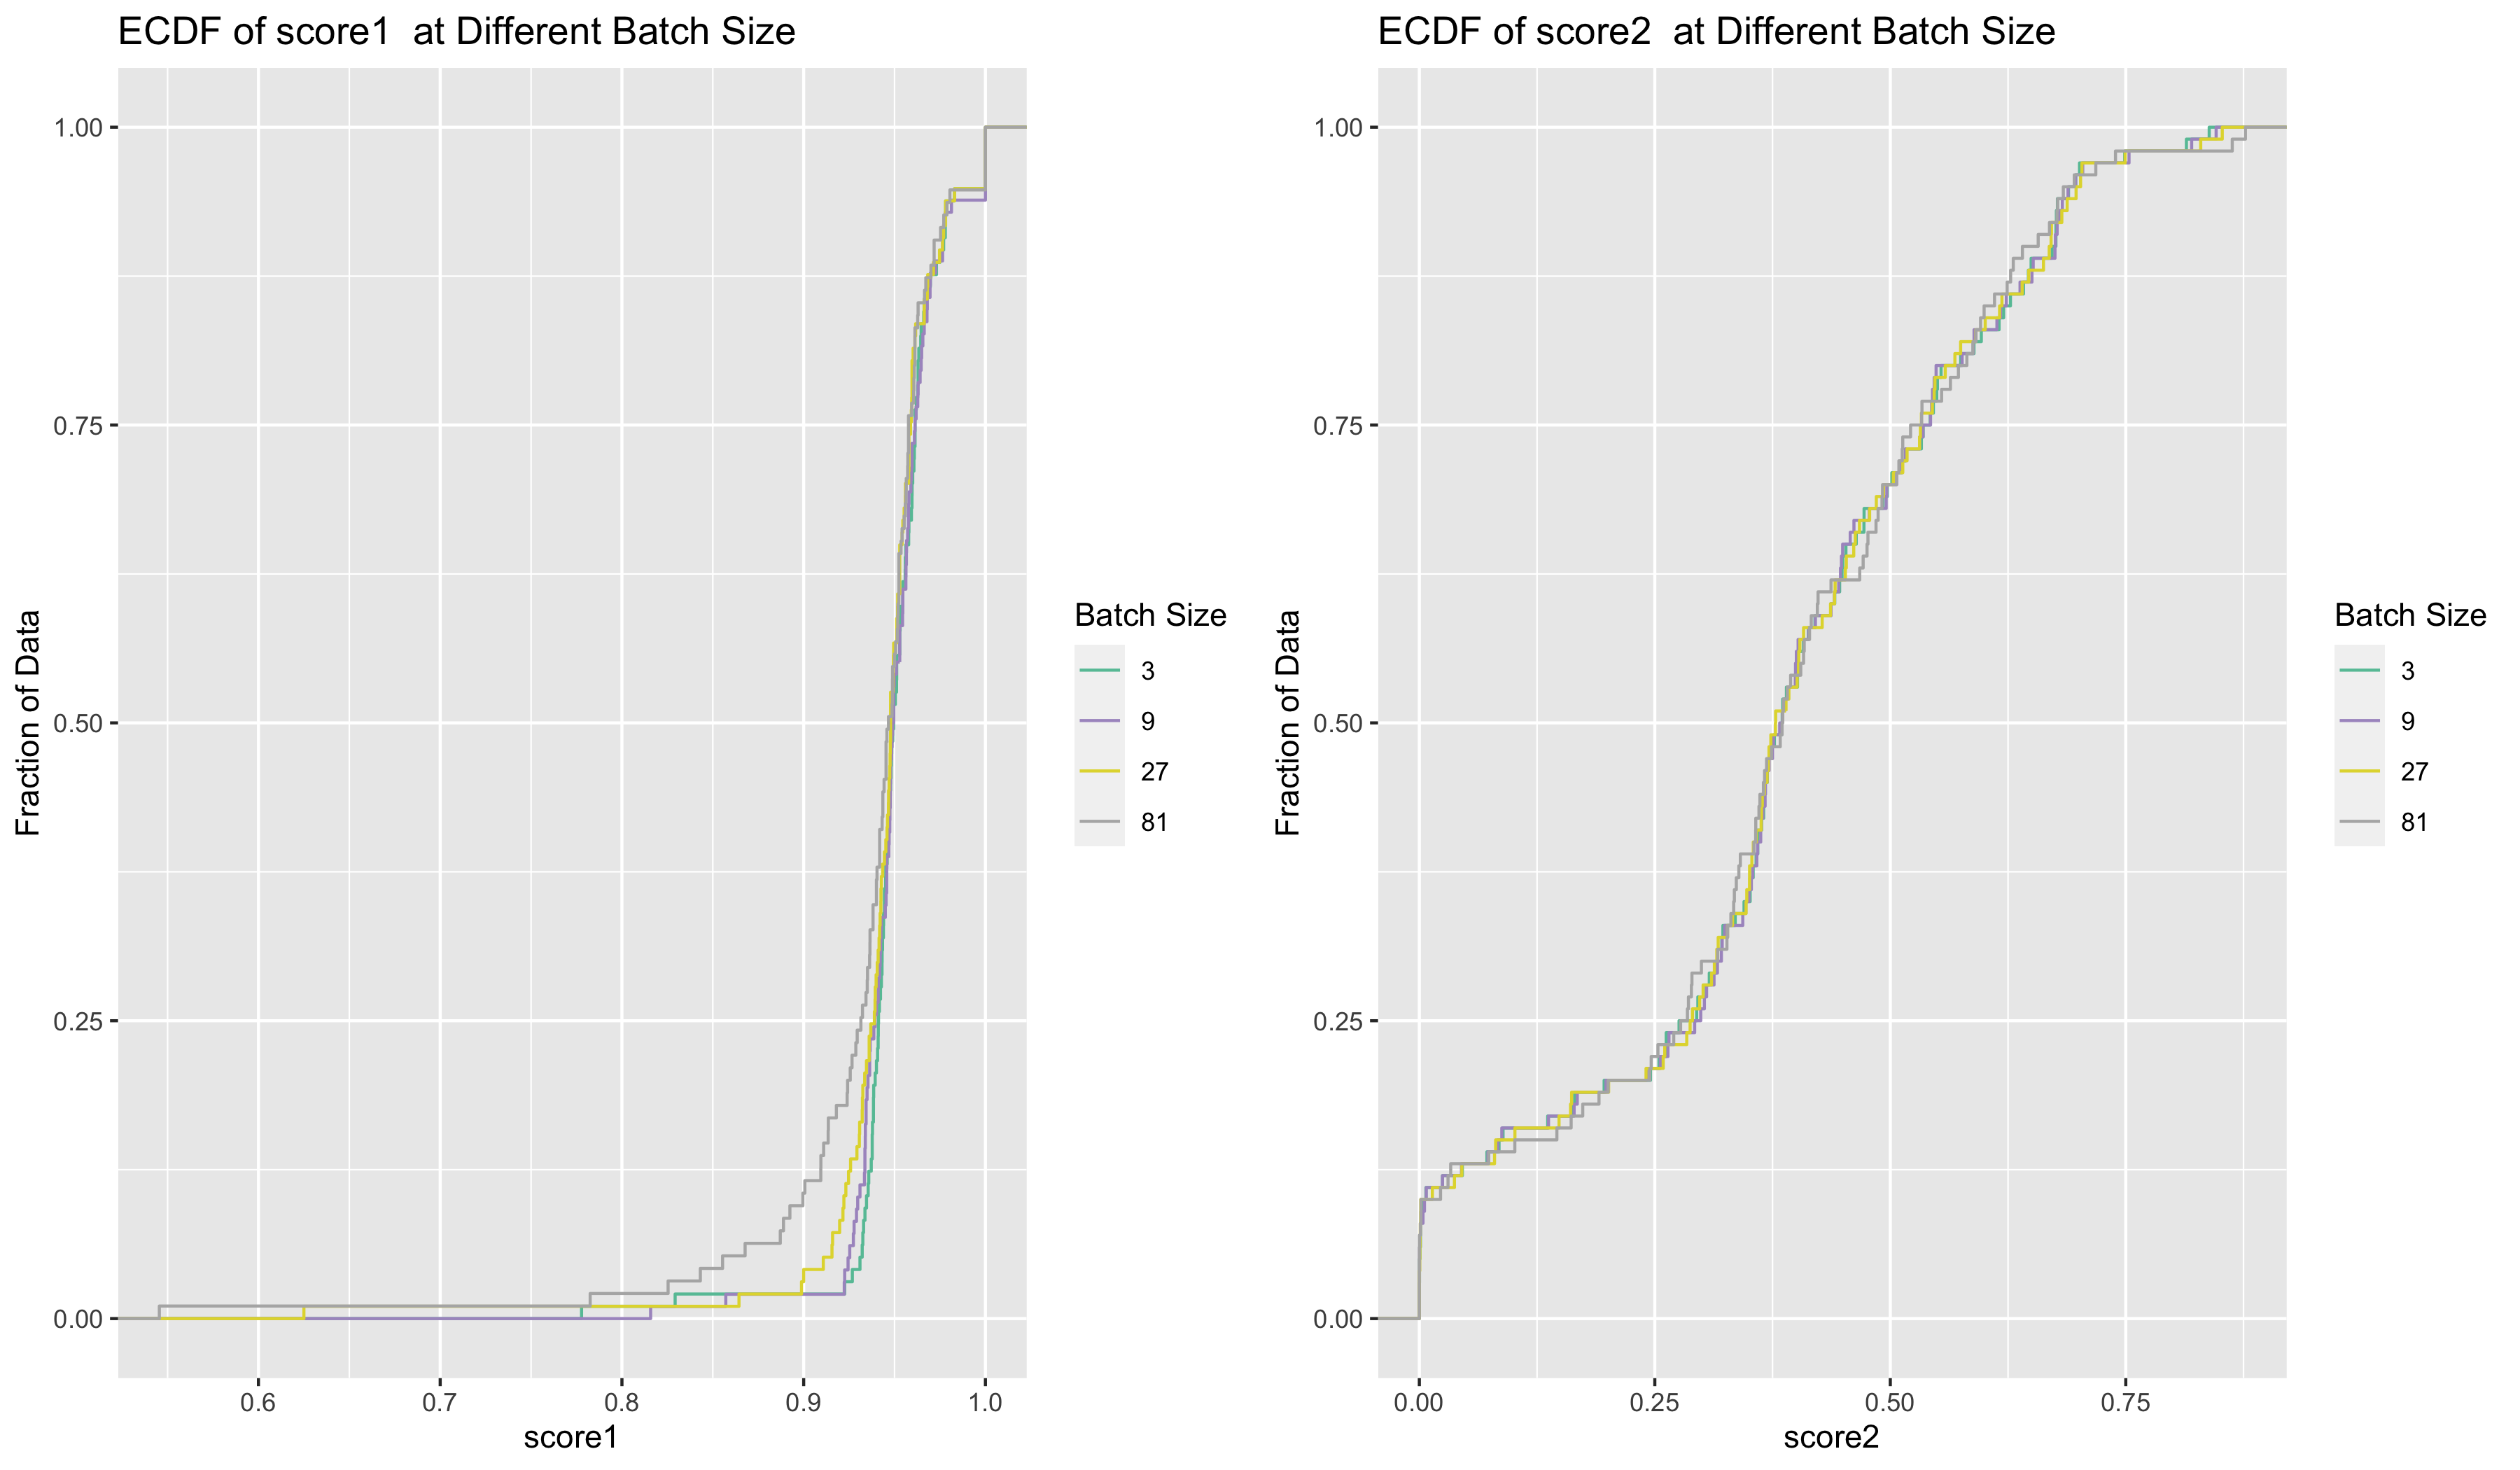
\includegraphics[width = 0.8\textwidth]{images/ECDFofscoresatDifferentBatchSizeOfAR1,840,1.png}
    \label{fig:fig1.5.2}
\end{figure}

\begin{table}[htbp]
  \begin{center}
    \caption{Configuration and Result of AR1 Model with Different Batch Size of Dynamic Training}
    \label{tab:tab1.5.2}
    \begin{tabular}{l|*{4}{c}}
      \textbf{batch size} & \textbf{score 1} & \textbf{score 1 weight} & \textbf{score 2} & \textbf{score 2 weight} \\
      \hline
      3 & 0.9508 & 47422 & 0.3844 & 59249\\
      9 & 0.9493 & 47562 & 0.3849 & 59249\\
      27 & 0.9468 & 47764 & 0.3847 & 59249\\
      81 & 0.9381 & 45813 & 0.3837 & 56561\\
    \end{tabular}
  \end{center}
\end{table}

\subsubsection{Parallel Models Policy}
Ref to Section 1.6, include Fig \ref{fig:fig1.6.1}, Table \ref{tab:tab1.6.1}, Fig \ref{fig:fig1.6.2}, Table \ref{tab:tab1.6.2}.

\begin{figure}
    \caption{ECDF of Scores for Different Model Number of Offline Training}
    \centering
    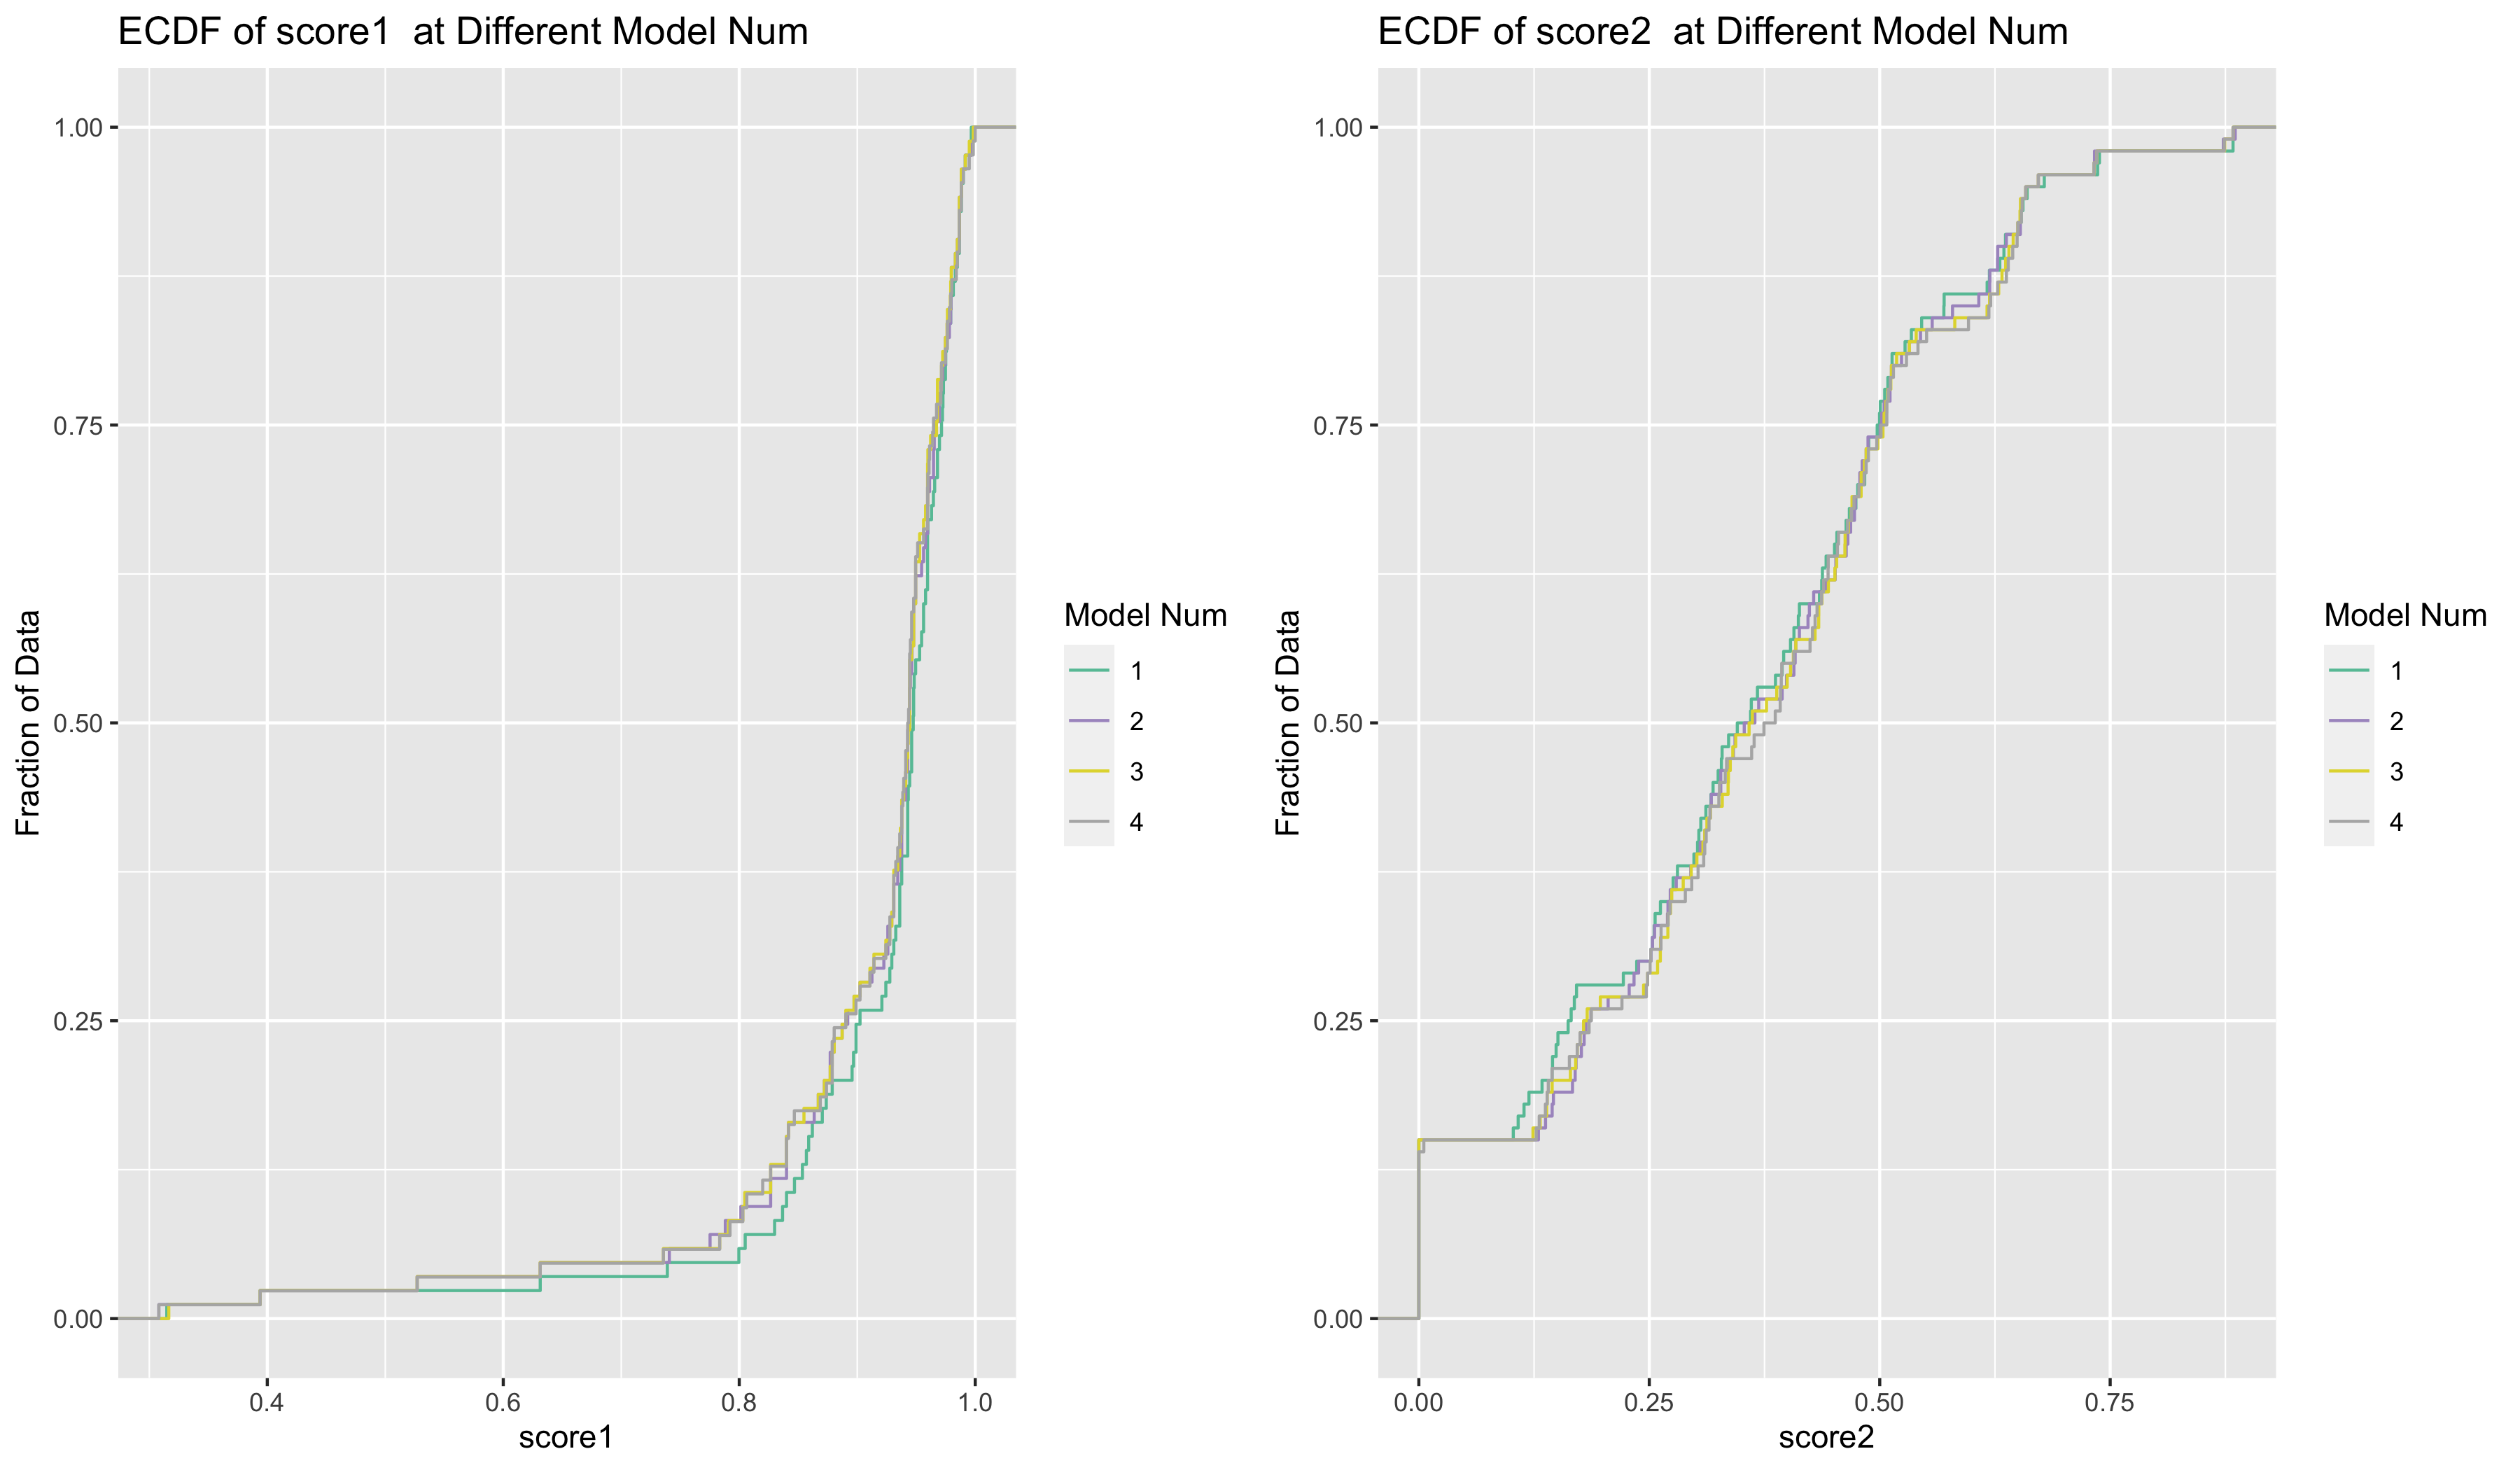
\includegraphics[width = 0.8\textwidth]{images/ECDFofscoresatDifferentModelNumOfAR1,840,3,offline.png}
    \label{fig:fig1.6.1}
\end{figure}

\begin{table}[htbp]
  \begin{center}
    \caption{Configuration and Result of AR1 Model with Different Model Number and Offline Training}
    \label{tab:tab1.6.1}
    \begin{tabular}{l|*{4}{c}}
      \textbf{model num} & \textbf{score 1} & \textbf{score 1 weight} & \textbf{score 2} & \textbf{score 2 weight} \\
      \hline
      1 & 0.9168 & 48124 & 0.3463 & 59249\\
      2 & 0.9108 & 48856 & 0.3537 & 59249\\
      3 & 0.9093 & 48606 & 0.3560 & 59249\\
      4 & 0.9090 & 48827 & 0.3574 & 59249\\
    \end{tabular}
  \end{center}
\end{table}

\begin{figure}
    \caption{ECDF of Scores for Different Model Number of Dynamic Training}
    \centering
    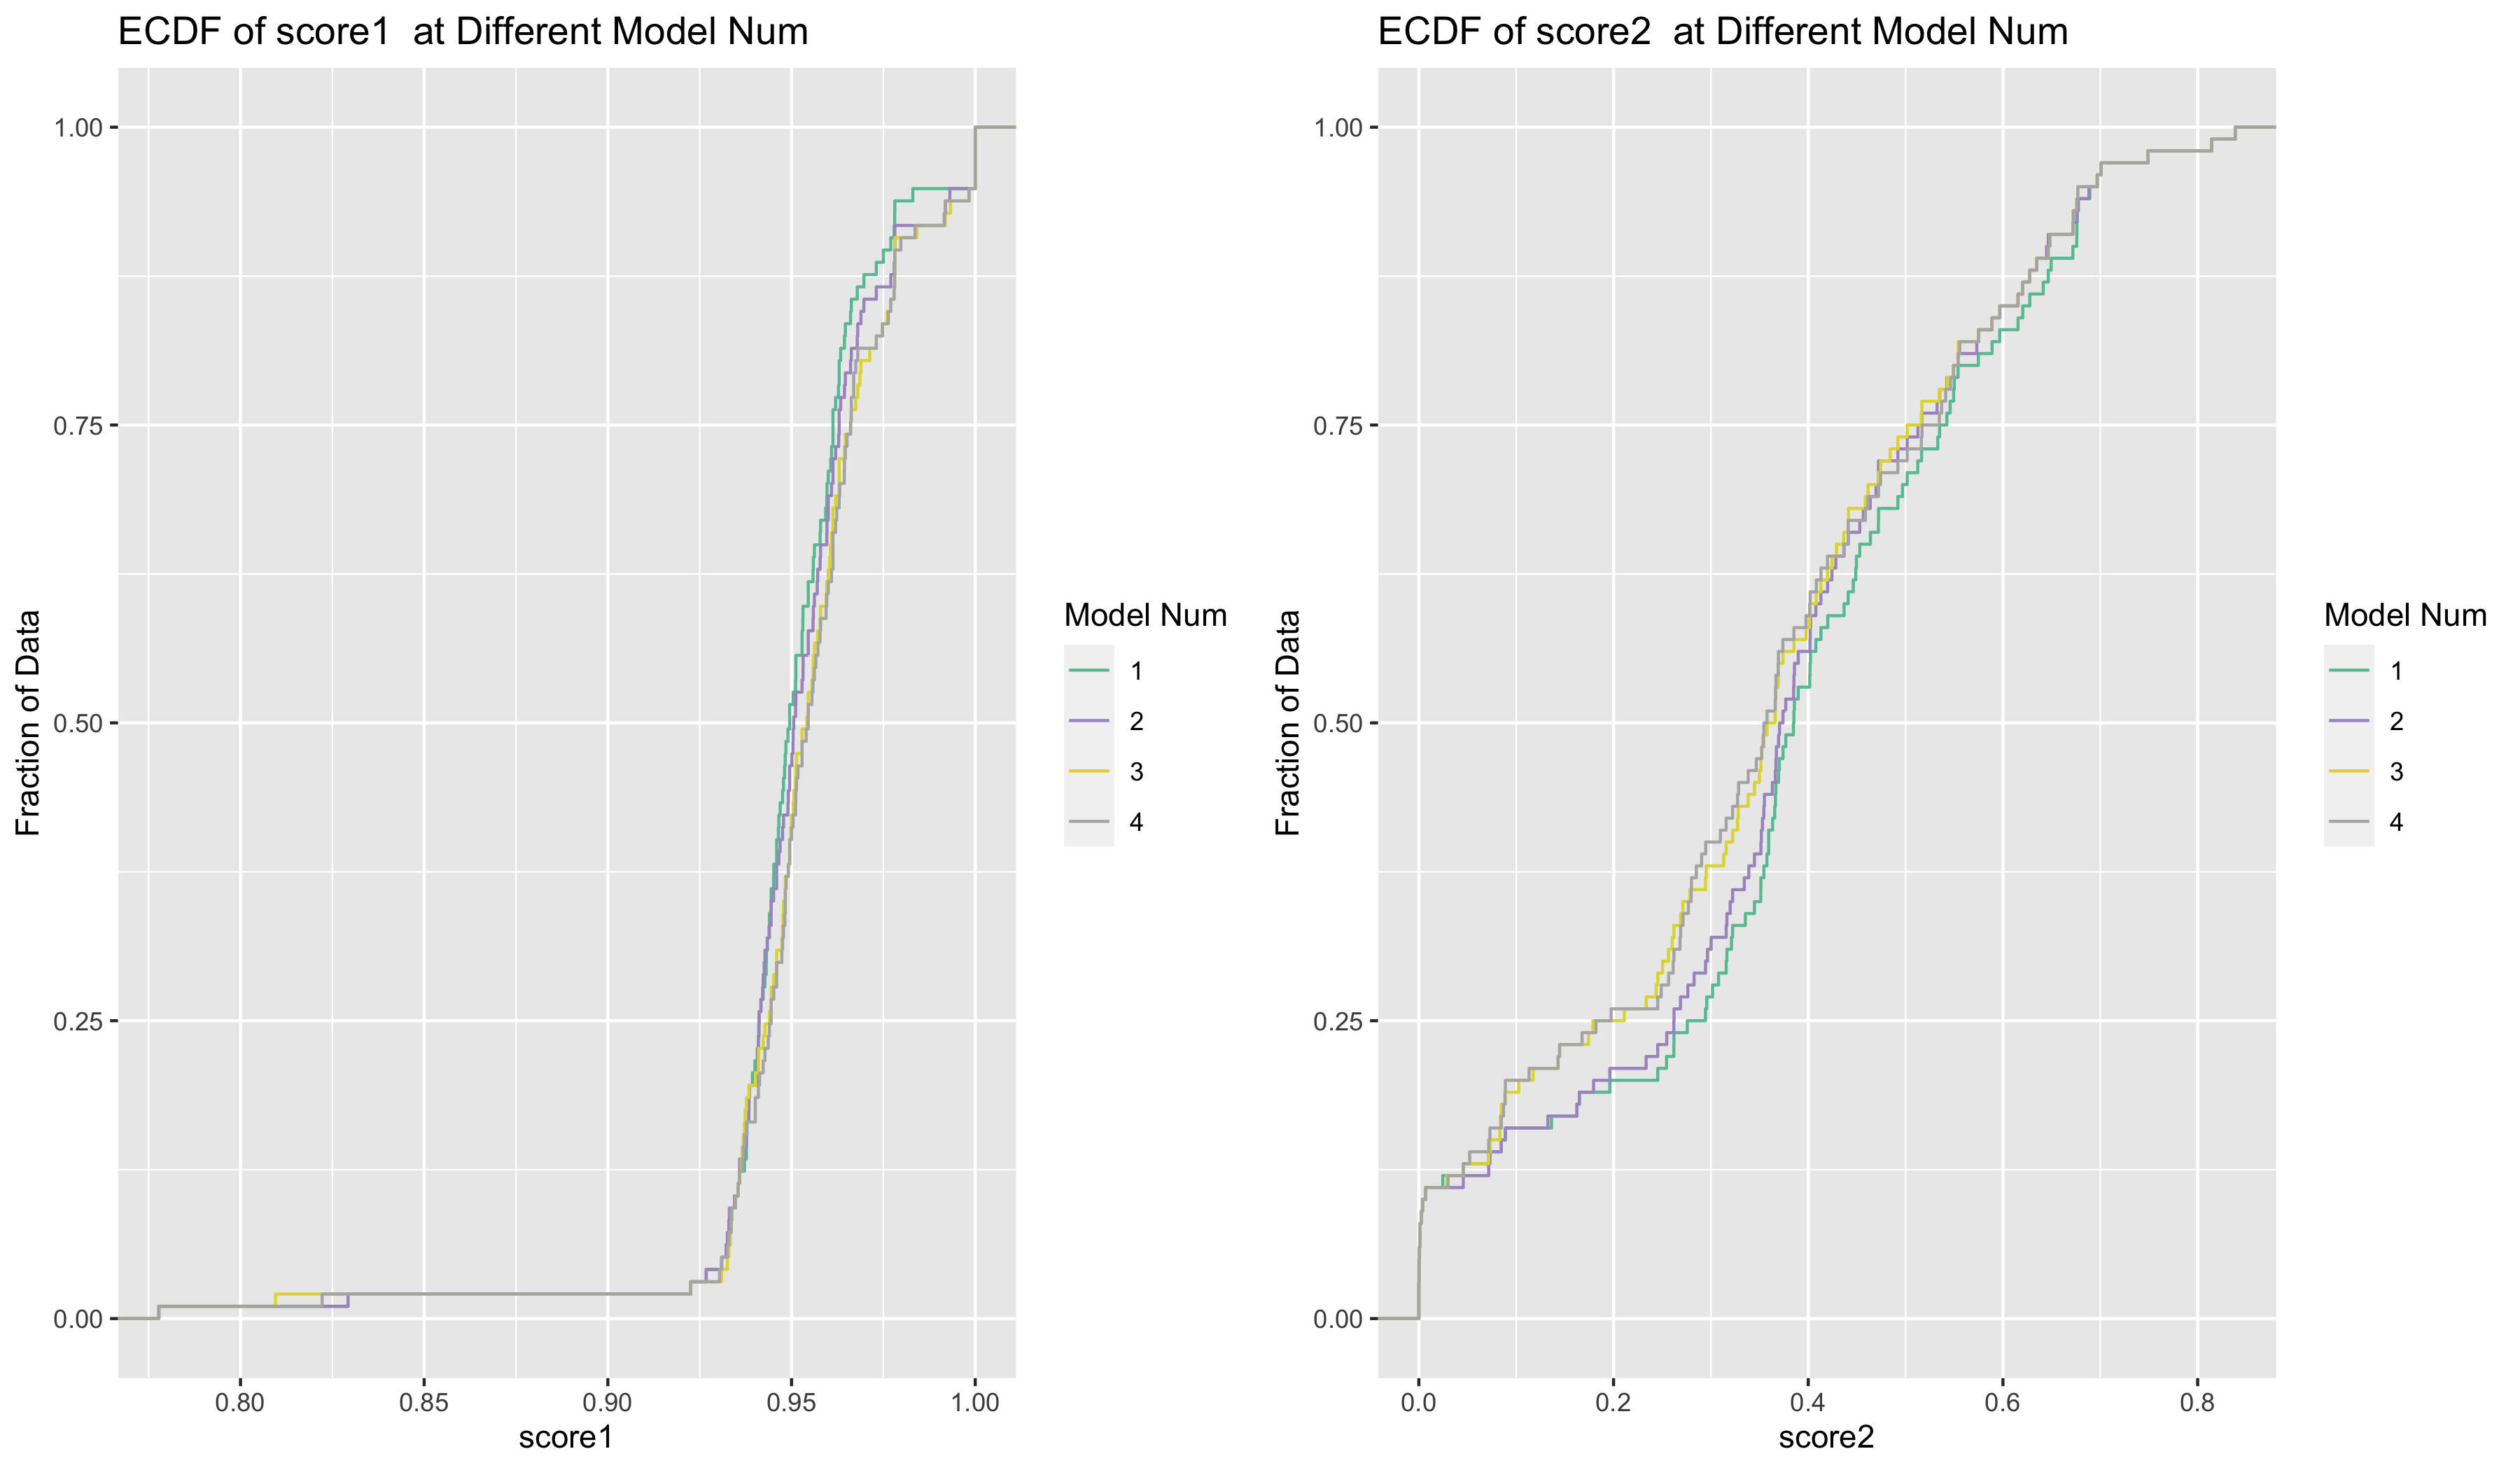
\includegraphics[width = 0.8\textwidth]{images/ECDFofscoresatDifferentModelNumOfAR1,840,3,dynamic.png}
    \label{fig:fig1.6.2}
\end{figure}

\begin{table}[htbp]
  \begin{center}
    \caption{Configuration and Result of AR1 Model with Different Model Number and Dynamic Training}
    \label{tab:tab1.6.2}
    \begin{tabular}{l|*{4}{c}}
      \textbf{model num} & \textbf{score 1} & \textbf{score 1 weight} & \textbf{score 2} & \textbf{score 2 weight} \\
      \hline
      1 & 0.9508 & 47422 & 0.3844 & 59249\\
      2 & 0.9527 & 47453 & 0.3716 & 59249\\
      3 & 0.9548 & 45913 & 0.3531 & 59249\\
      4 & 0.9551 & 45760 & 0.3527 & 59249\\
    \end{tabular}
  \end{center}
\end{table}

\subsubsection{Granularity}
Ref to Section 1.7, include Fig \ref{fig:fig1.7.1}, Table \ref{tab:tab1.7.1}.

\begin{figure}
    \caption{ECDF of Scores for Different Granularity of Offline Training}
    \centering
    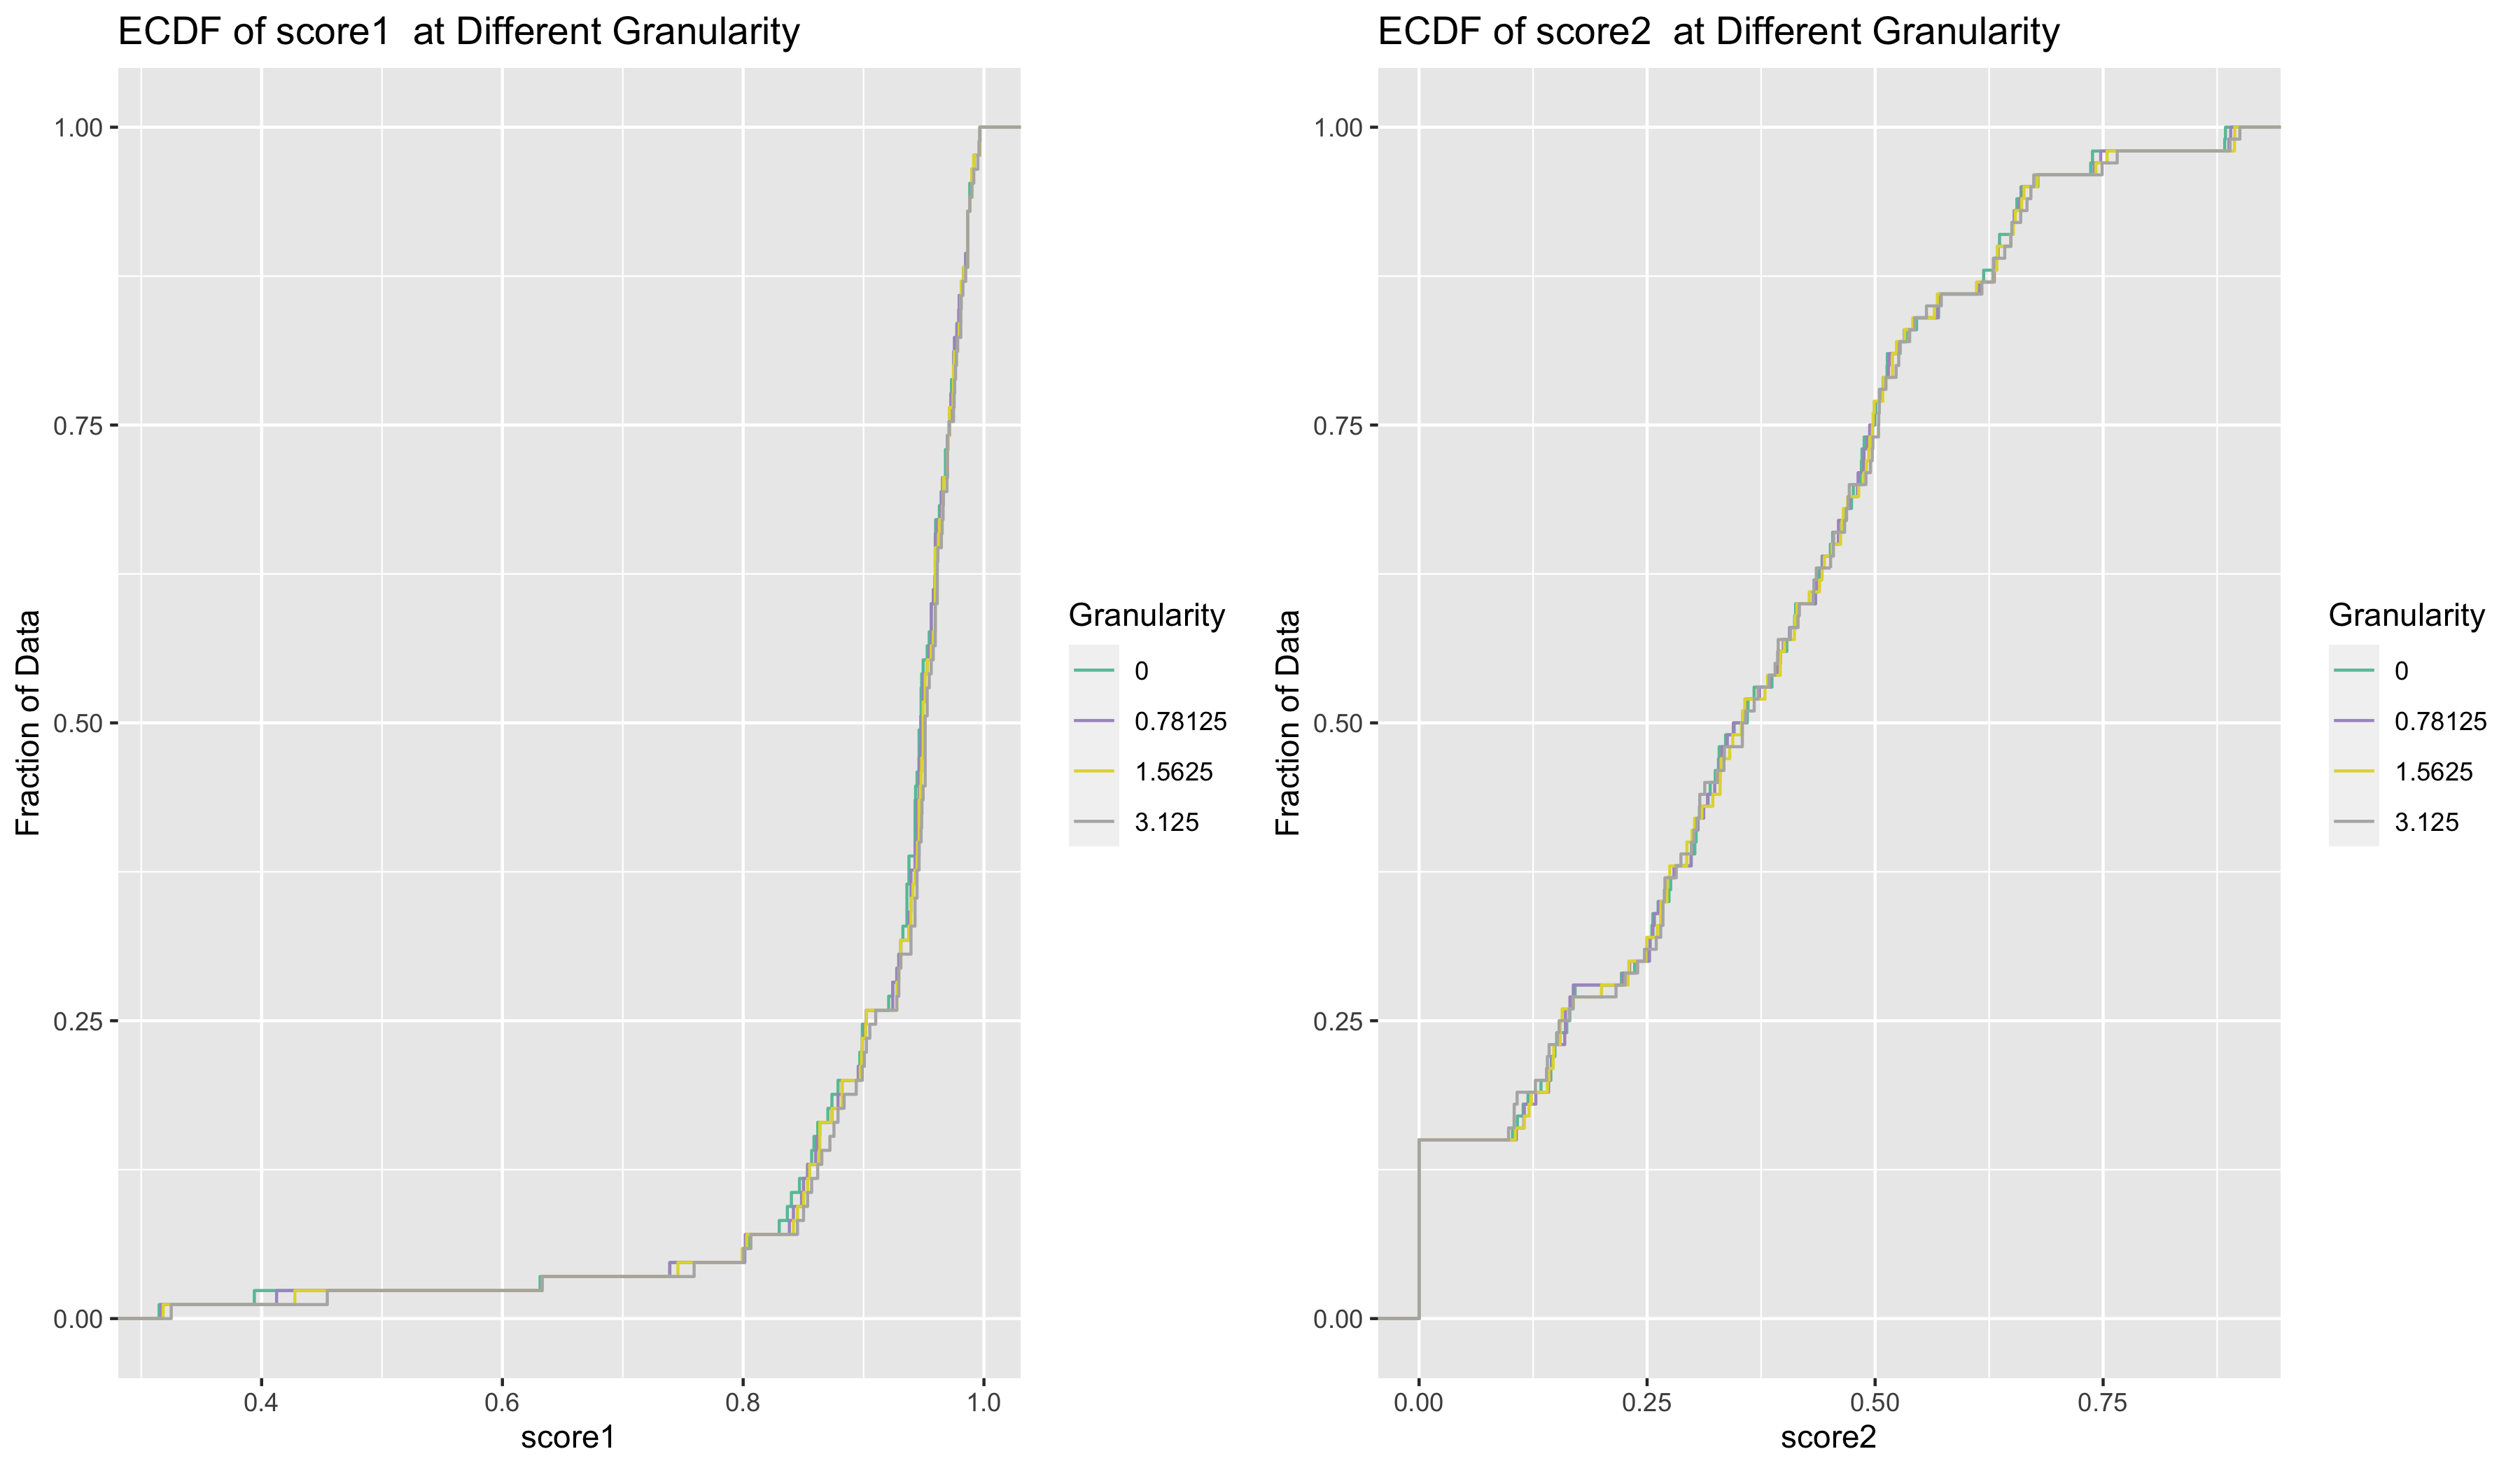
\includegraphics{images/ECDFofscoresatDifferentGranularityOfAR1,840,3,1.png}
    \label{fig:fig1.7.1}
\end{figure}

\begin{table}[htbp]
  \begin{center}
    \caption{Configuration and Result of AR1 Model with Different Granularity and Offline Training}
    \label{tab:tab1.7.1}
    \begin{tabular}{l|*{4}{c}}
      \textbf{granularity} & \textbf{score 1} & \textbf{score 1 weight} & \textbf{score 2} & \textbf{score 2 weight} \\
      \hline
      0 & 0.9168 & 48124 & 0.3463 & 59249\\
      0.78125 & 0.9183 & 48070 & 0.3577 & 57170\\
      1.5625 & 0.9197 & 47992 & 0.3638 & 56005\\
      3.125 & 0.9224 & 47725 & 0.3667 & 55163\\
    \end{tabular}
  \end{center}
\end{table}

\subsubsection{Adjustment Policy}
Ref to Section 1.8

\begin{figure}
    \caption{ECDF of Scores for Different React Speed of Adjustment Policy of Offline Training}
    \centering
    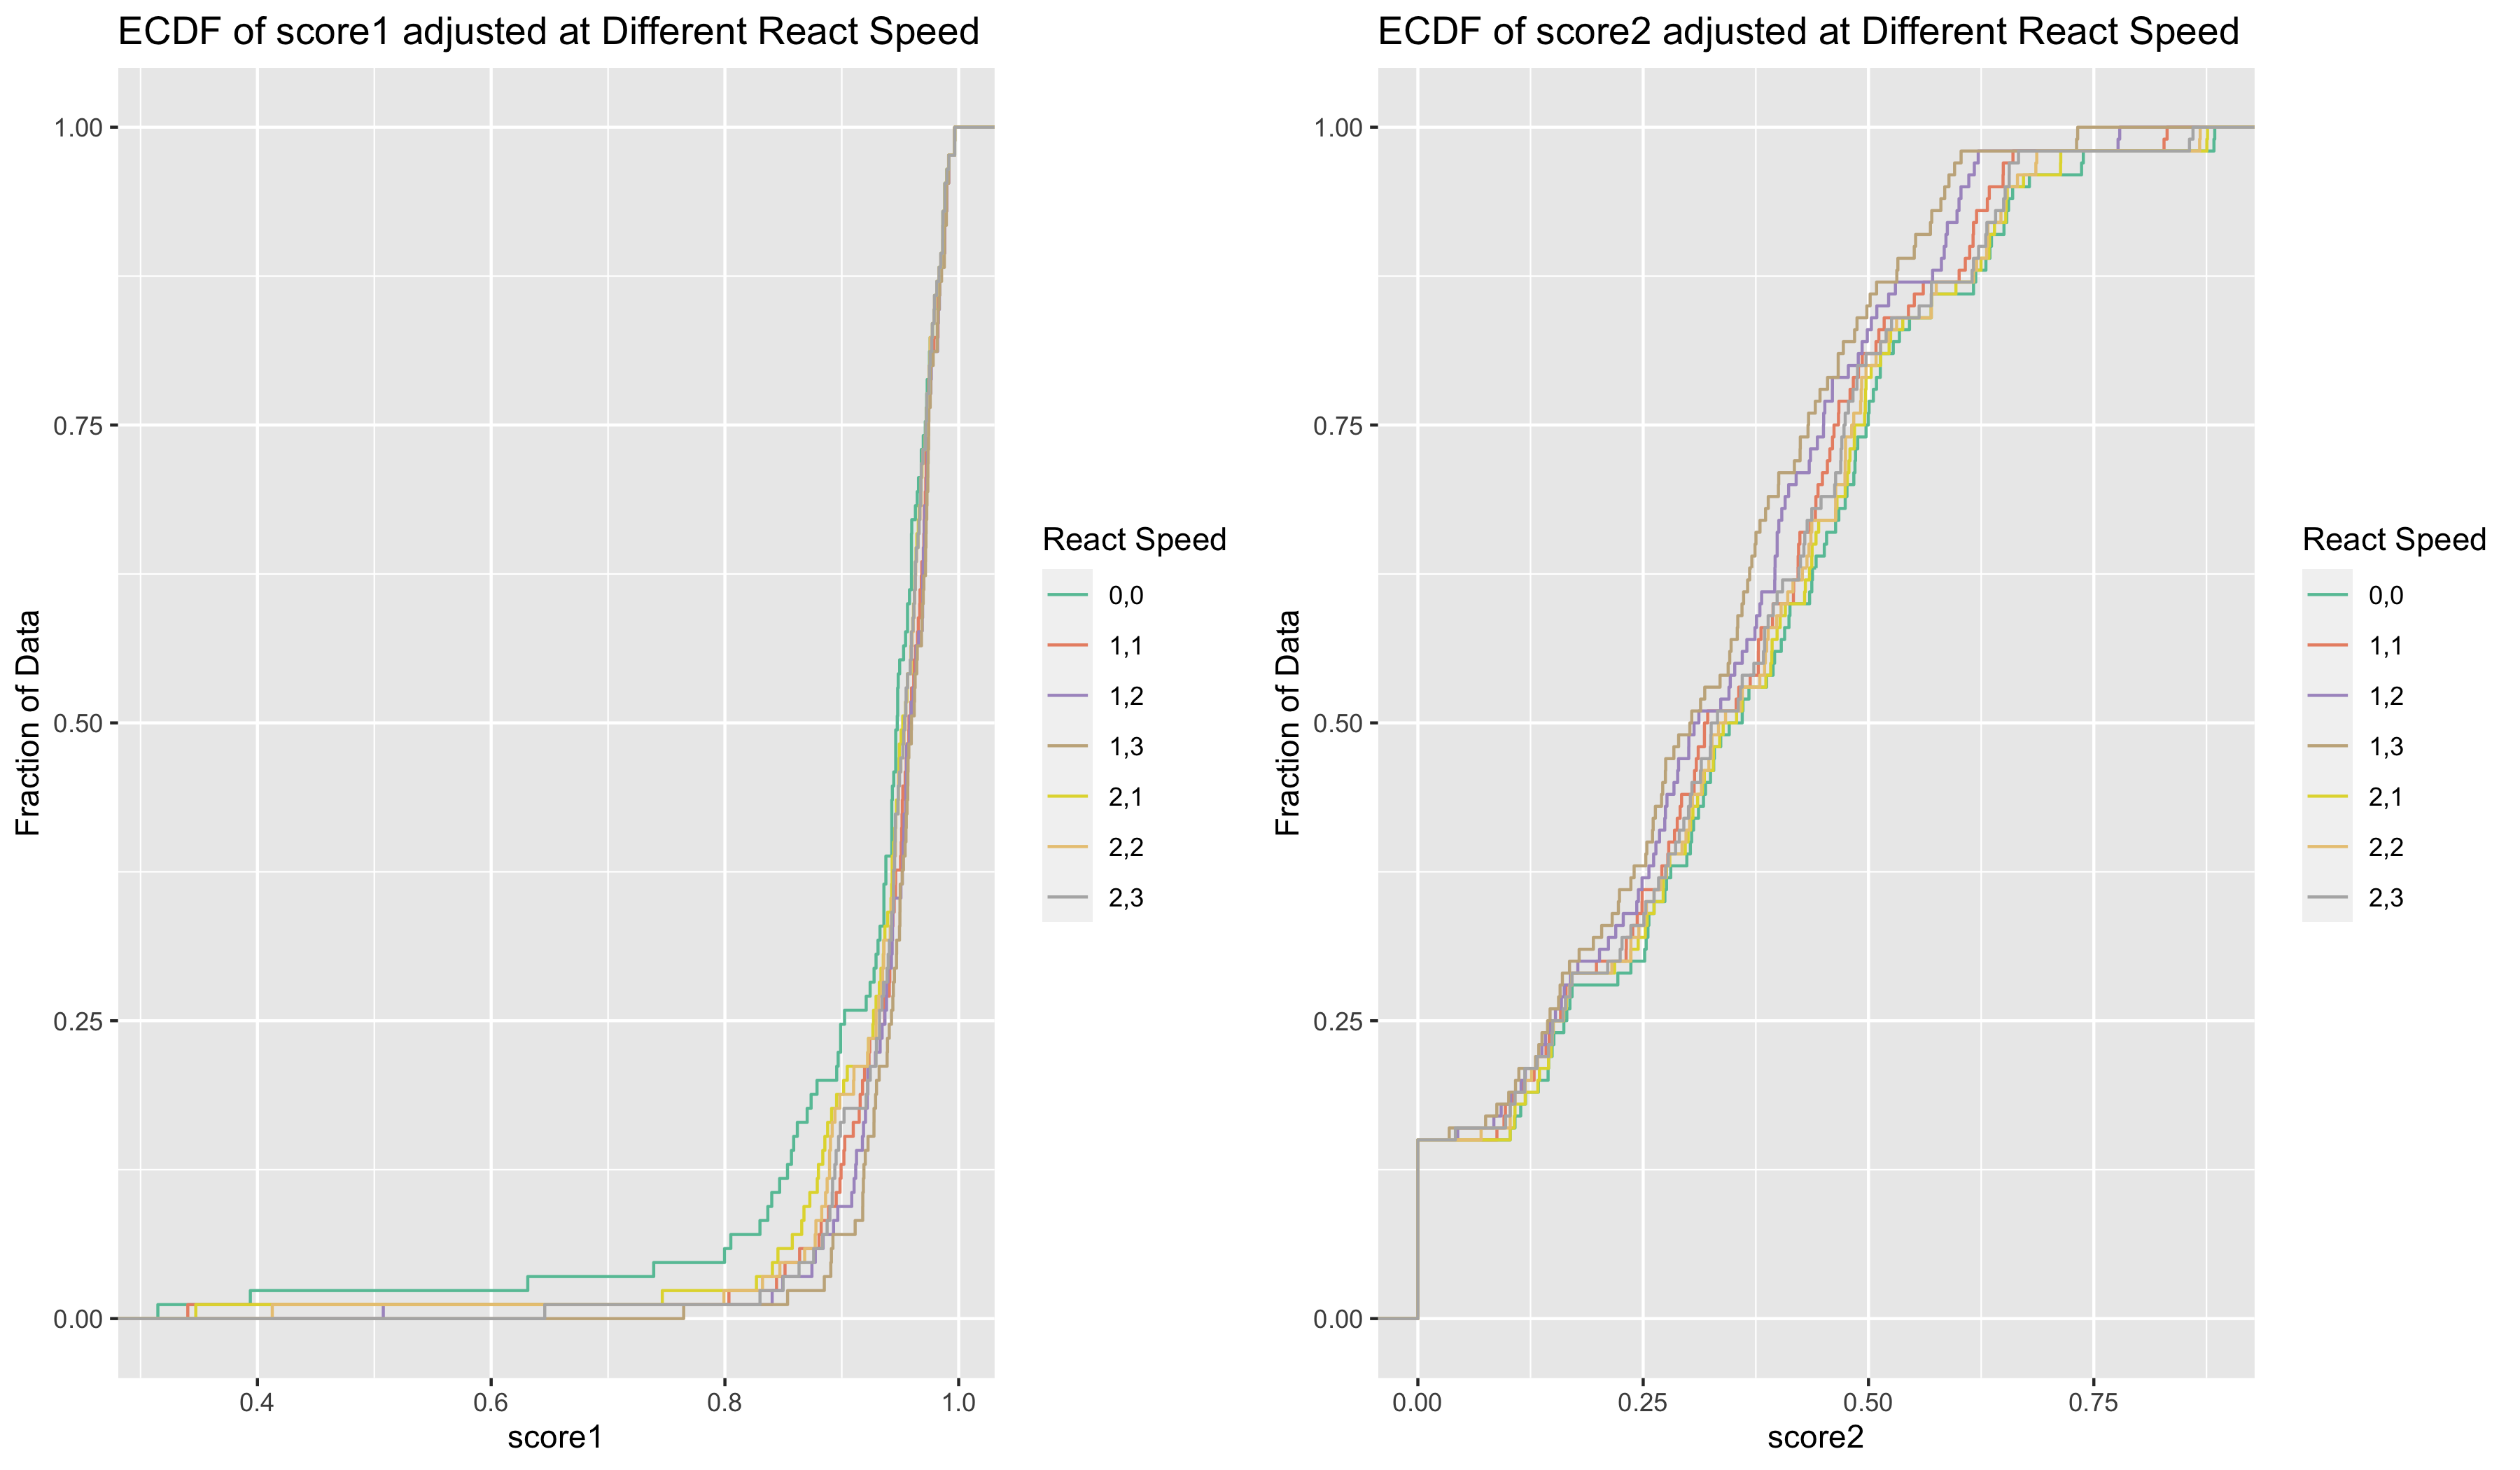
\includegraphics{images/ECDFofscoresadjustedatDifferentReactSpeedOfAR1,840,3,1.png}
    \label{fig:fig1.8.1}
\end{figure}

\begin{table}[htbp]
  \begin{center}
    \caption{Configuration and Result of AR1 Model with Different React Speed of Adjustment Policy of Offline Training}
    \label{tab:tab1.8.1}
    \begin{tabular}{l|*{4}{c}}
      \textbf{react speed} & \textbf{score 1} & \textbf{score 1 weight} & \textbf{score 2} & \textbf{score 2 weight} \\
      \hline
      0,0 & 0.9168 & 48124 & 0.3463 & 59249\\
      1,1 & 0.9486 & 44126 & 0.3258 & 59249\\
      1,2 & 0.9544 & 41871 & 0.3092 & 59249\\
      1,3 & 0.9589 & 39976 & 0.2952 & 59249\\
      2,1 & 0.9392 & 46387 & 0.3407 & 59249\\
      2,2 & 0.9448 & 45564 & 0.3355 & 59249\\
      2,3 & 0.9487 & 44804 & 0.3463 & 59249\\
    \end{tabular}
  \end{center}
\end{table}


\subsubsection{Cut-off Probability}
Ref to Section 1.9, include Fig \ref{fig:fig1.9.1}, Table \ref{tab:tab1.9.1}.

\begin{figure}
    \caption{ECDF of Scores for Different Cut Off Probability}
    \centering
    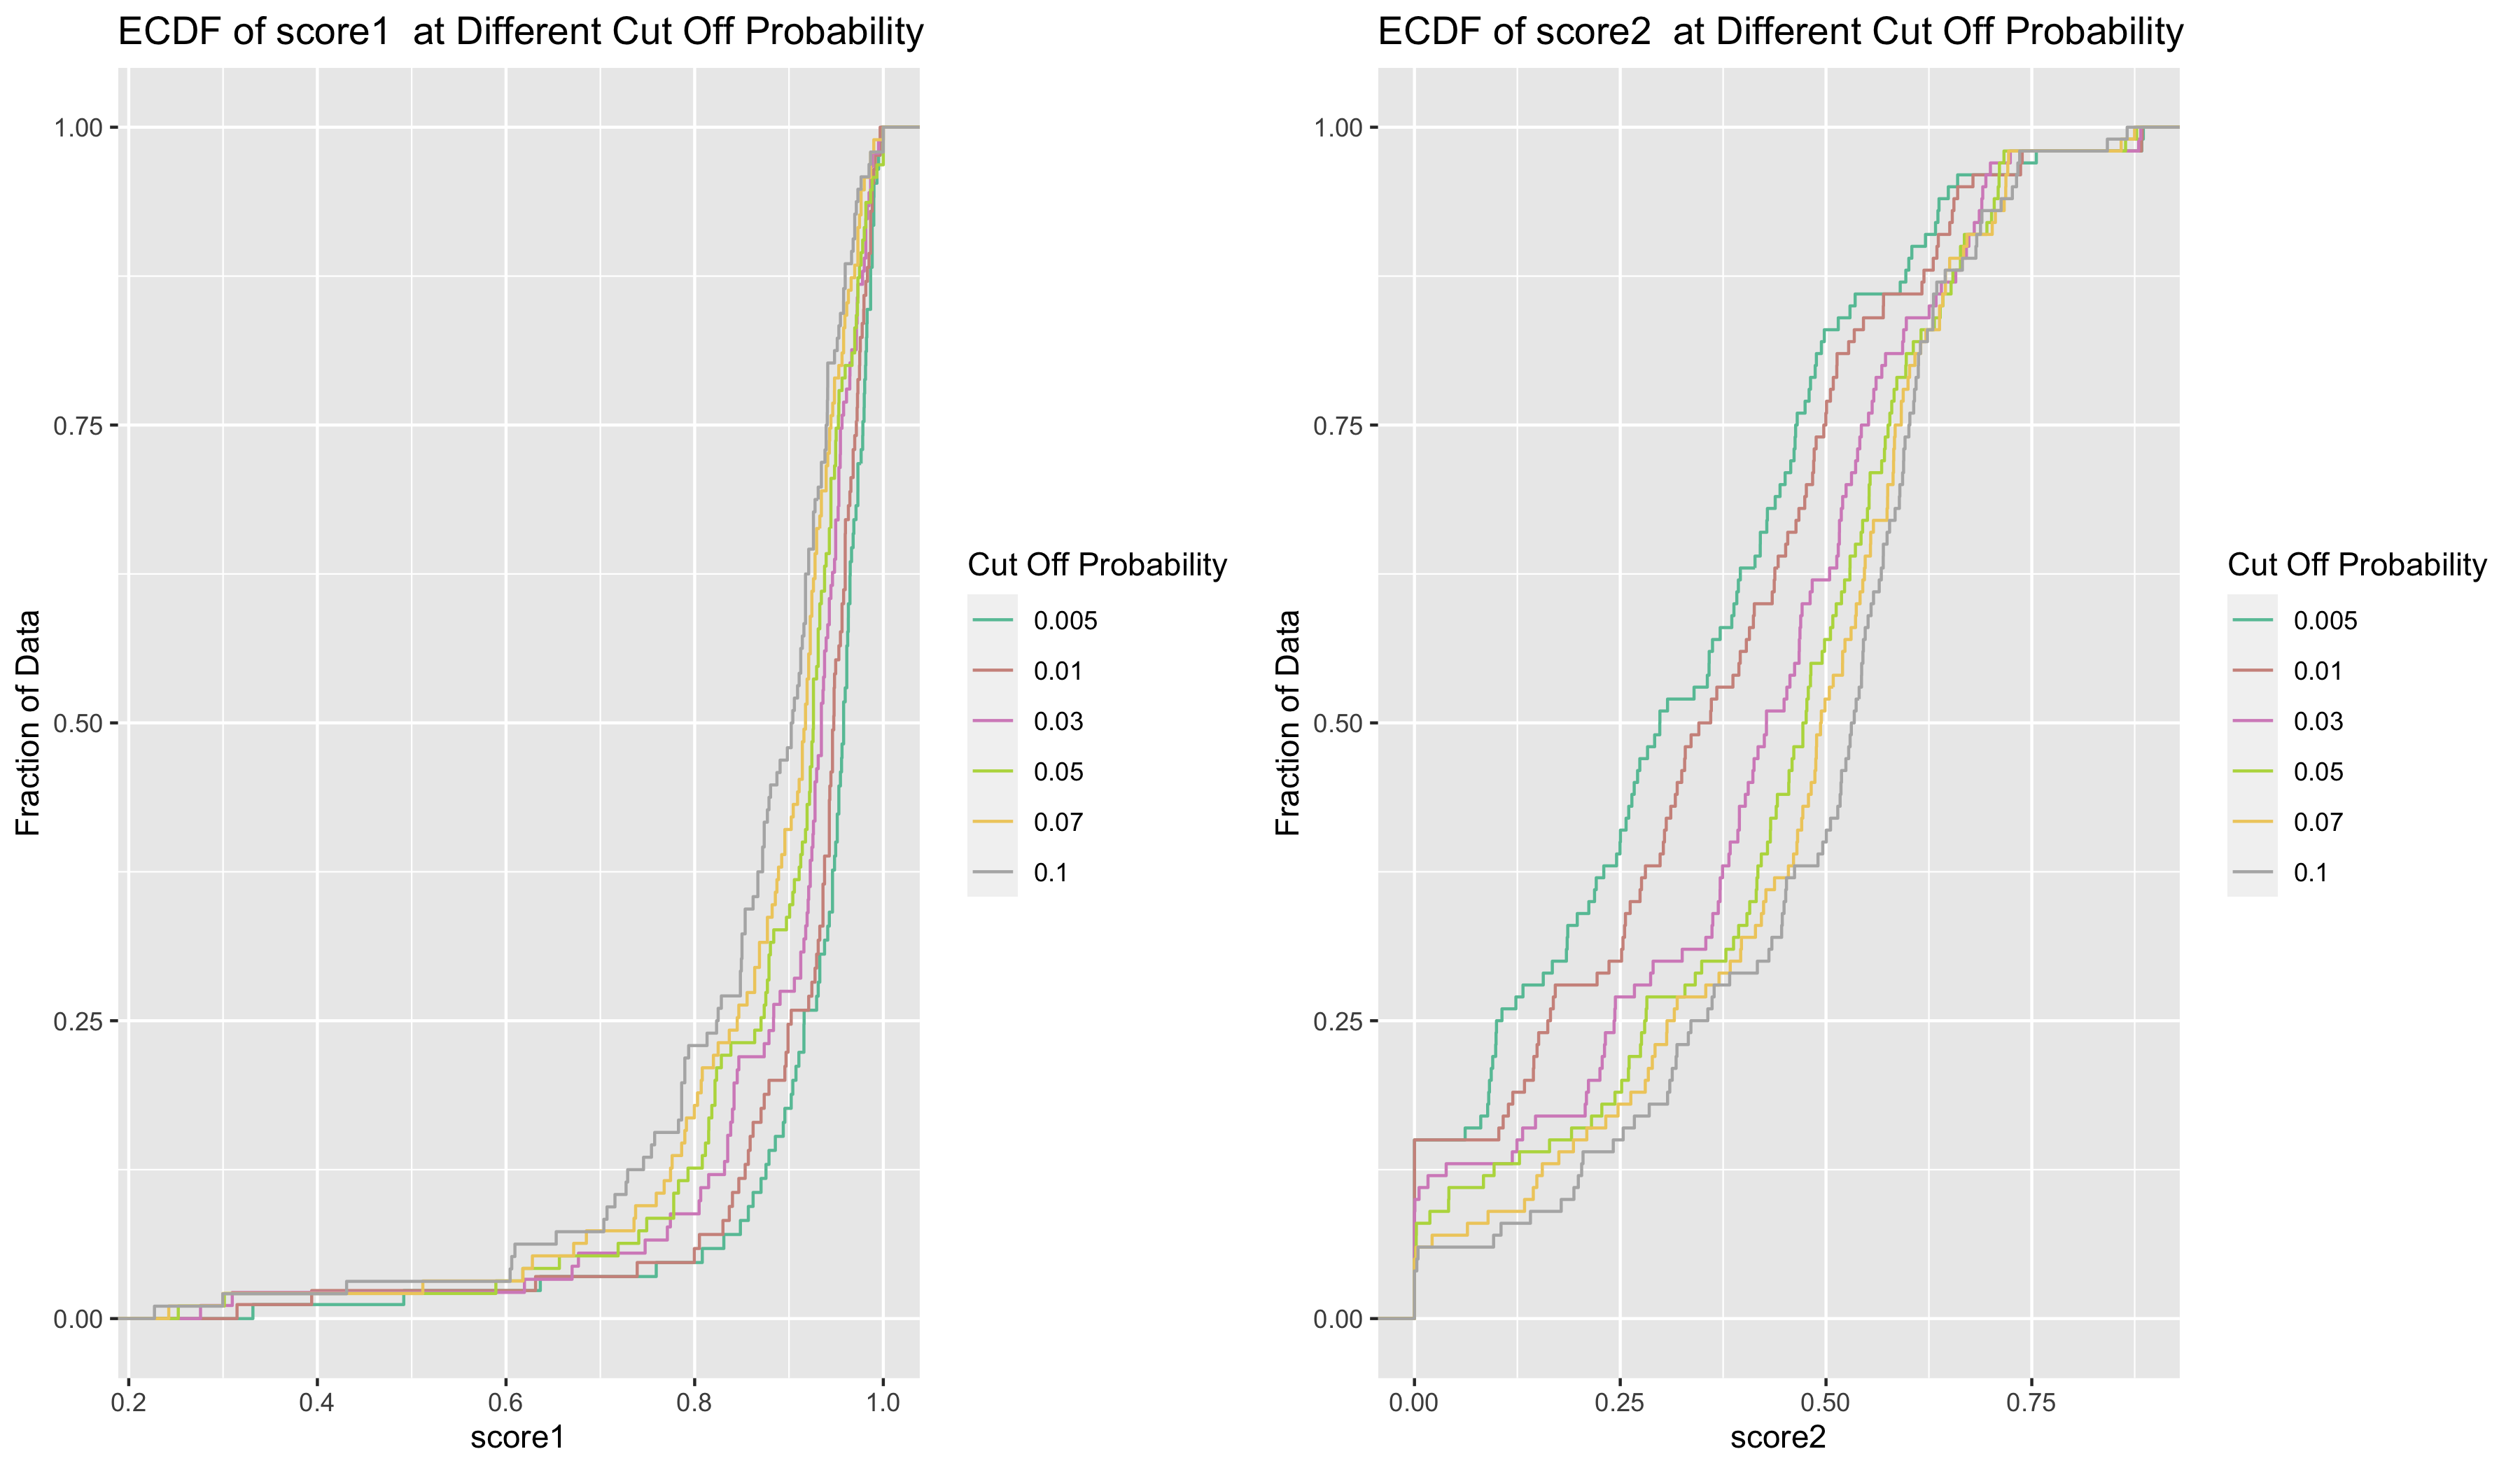
\includegraphics{images/ECDFofscoresatDifferentCutOffProbabilityOfAR1,840,3,1.png}
    \label{fig:fig1.9.1}
\end{figure}

\begin{table}[htbp]
  \begin{center}
    \caption{Configuration and Result of AR1 Model with Different Cut Off Probability of Offline Training}
    \label{tab:tab1.9.1}
    \begin{tabular}{l|*{4}{c}}
      \textbf{cut off prob} & \textbf{score 1} & \textbf{score 1 weight} & \textbf{score 2} & \textbf{score 2 weight} \\
      \hline
      0.005 & 0.9277 & 47487 & 0.3142 & 59249\\
      0.01 & 0.9168 & 48124 & 0.3463 & 59249\\
      0.03 & 0.8965 & 50300 & 0.4024 & 59249\\
      0.05 & 0.8841 & 52904 & 0.4309 & 59249\\
      0.07 & 0.8706 & 53640 & 0.4518 & 59249\\
      0.10 & 0.8548 & 54444 & 0.4729 & 59249\\
    \end{tabular}
  \end{center}
\end{table}

\subsubsection{Predicting Average of Next Window}
Ref to Section 1.10, include Fig \ref{fig:fig1.10.1}, Table \ref{fig:fig1.10.1}, Fig \ref{fig:fig1.10.2}, Table \ref{tab:tab1.10.2}.

\begin{figure}
    \caption{ECDF of Scores for Different Models Predicting Averages of Next Window with Offline Training}
    \centering
    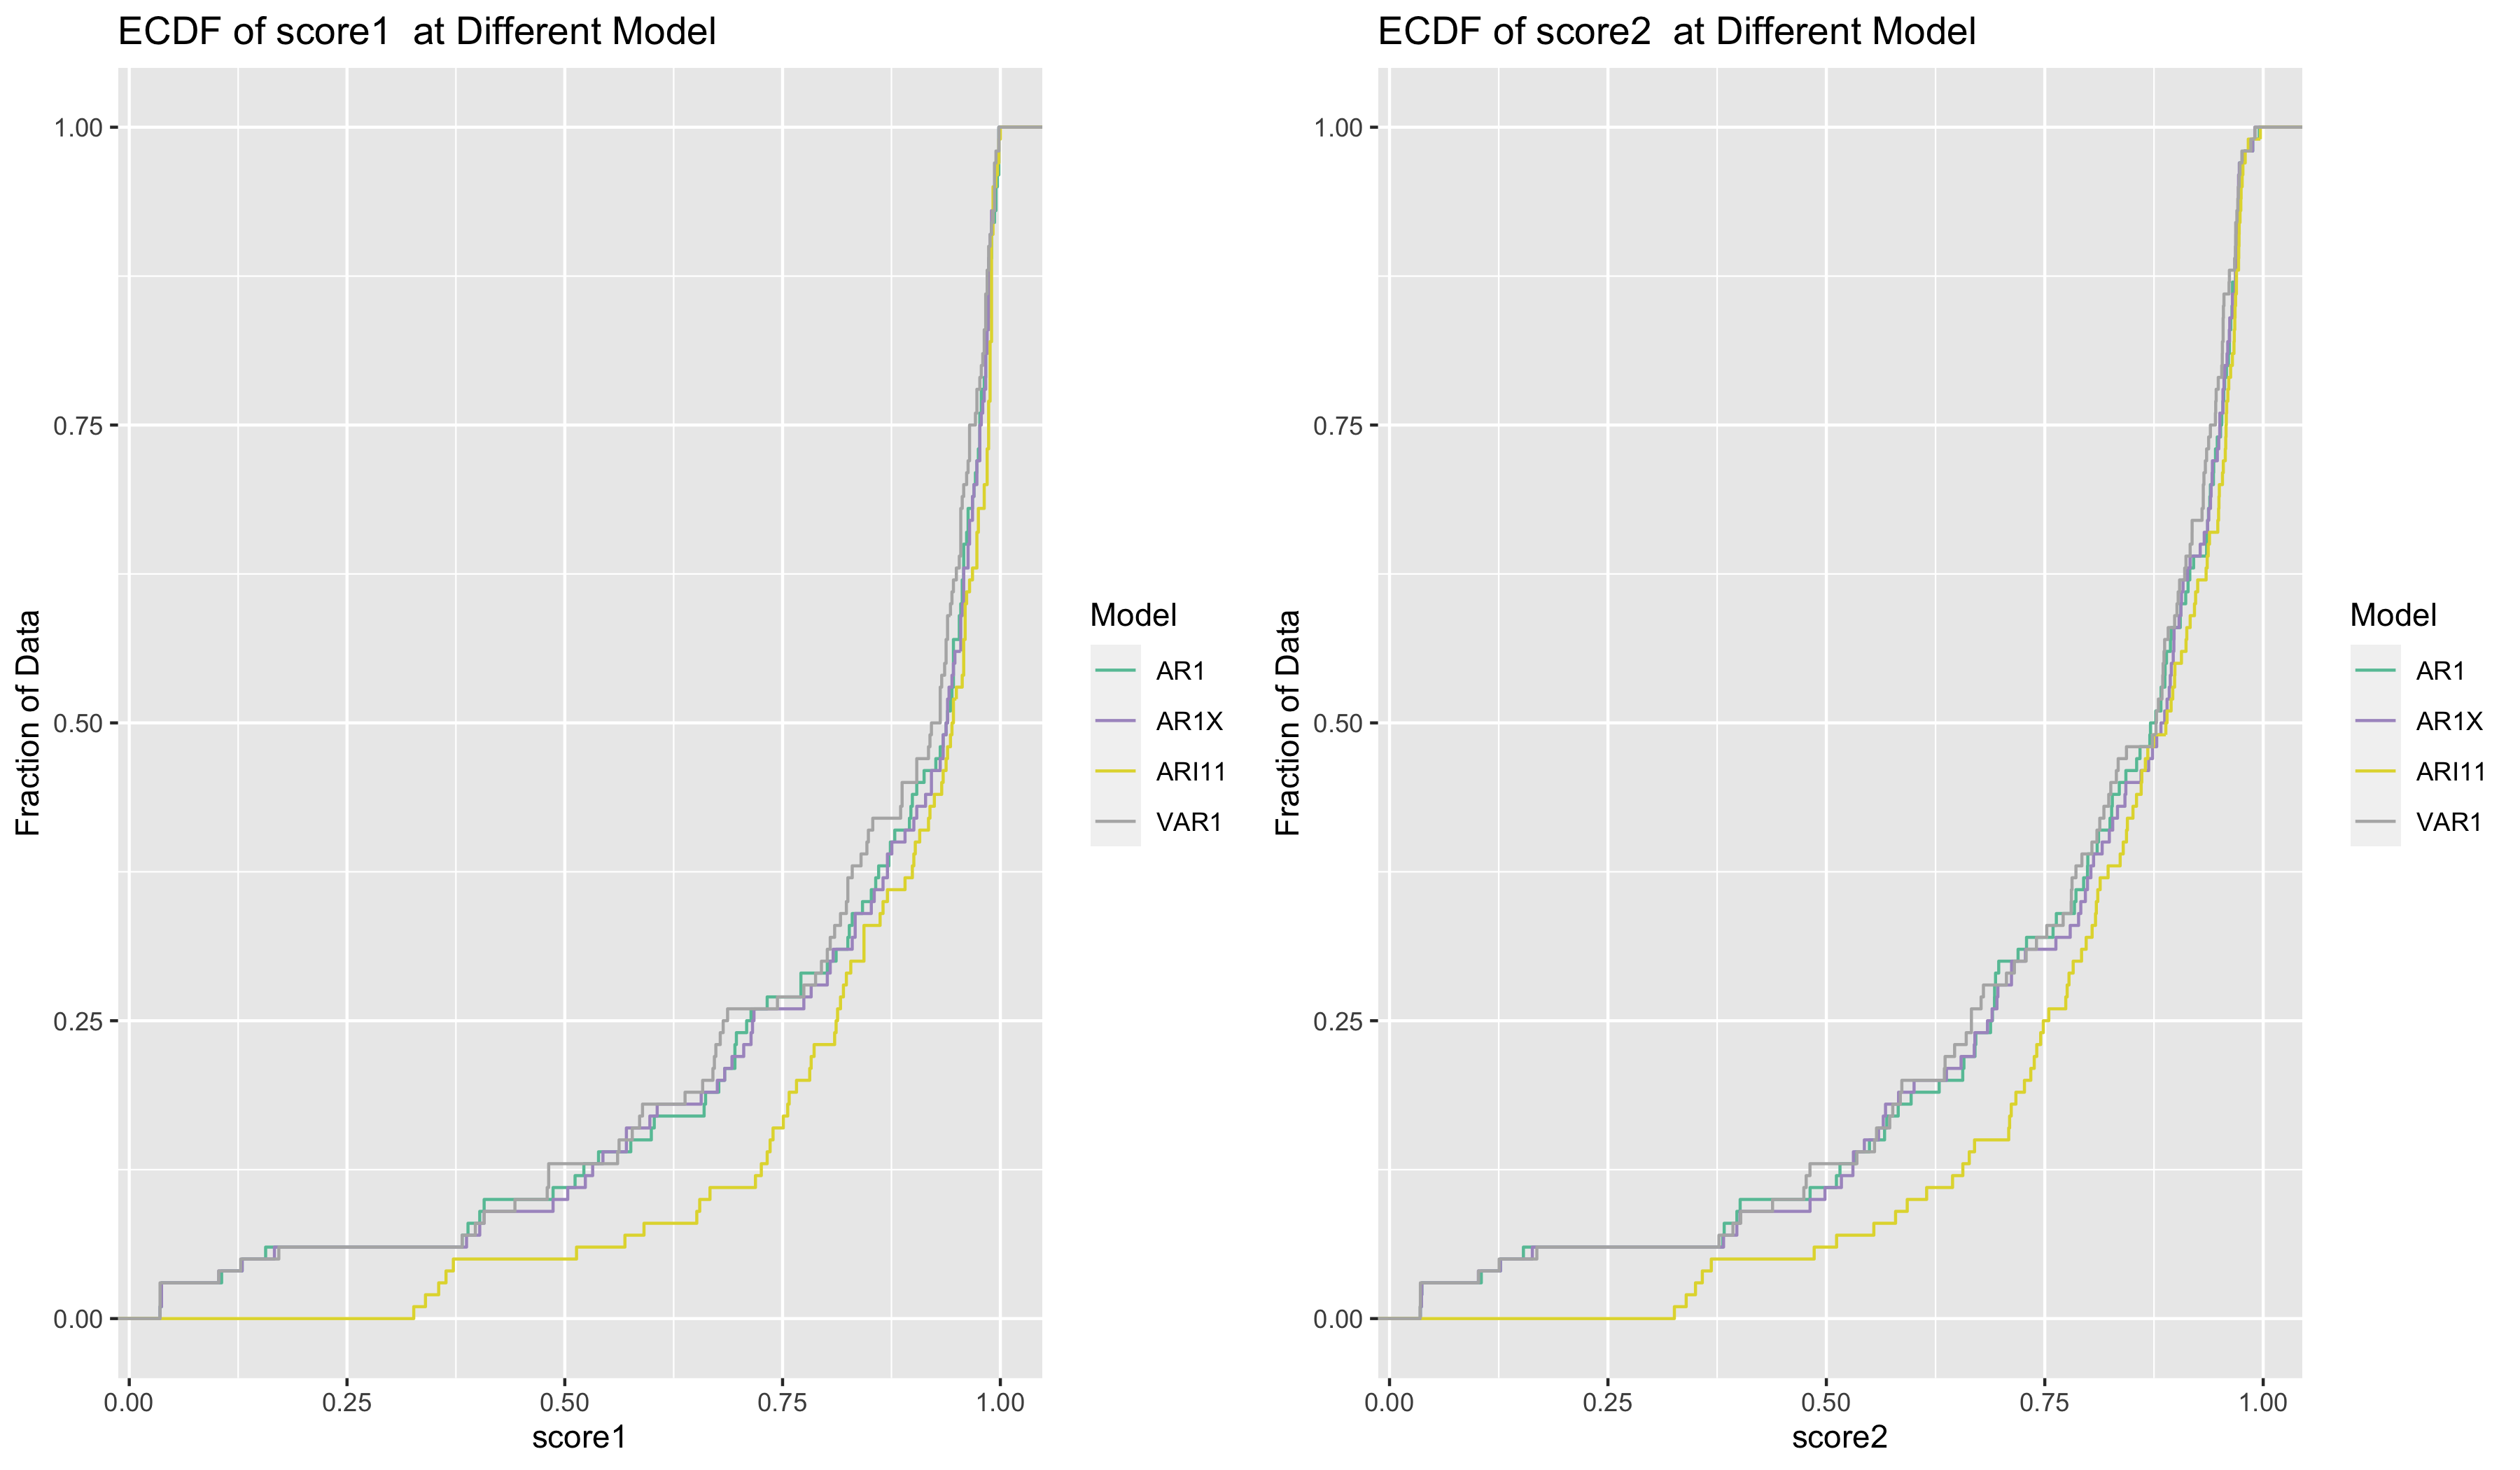
\includegraphics{images/ECDFofscoresatDifferentModelOfAR1,AR1X,ARI11,VAR1.png}
    \label{fig:fig1.10.1}
\end{figure}

\begin{table}[htbp]
  \begin{center}
    \caption{Configuration and Result of Different Models Predicting Averages of Next Window with Offline Training}
    \label{tab:tab1.10.1}
    \begin{tabular}{l|*{4}{c}}
      \textbf{model} & \textbf{score 1} & \textbf{score 1 weight} & \textbf{score 2} & \textbf{score 2 weight} \\
      \hline
      AR1 & 0.8141 & 59399 & 0.7768 & 59400\\
      AR1X & 0.8174 & 59399 & 0.7800 & 59400\\
      ARI11 & 0.8716 & 59399 & 0.8308 & 59400\\
      VAR1 & 0.8041 & 59399 & 0.7706 & 59400\\
    \end{tabular}
  \end{center}
\end{table}

\begin{figure}
    \caption{ECDF of Scores for Different Models Predicting Averages of Next Window with Offline Training}
    \centering
    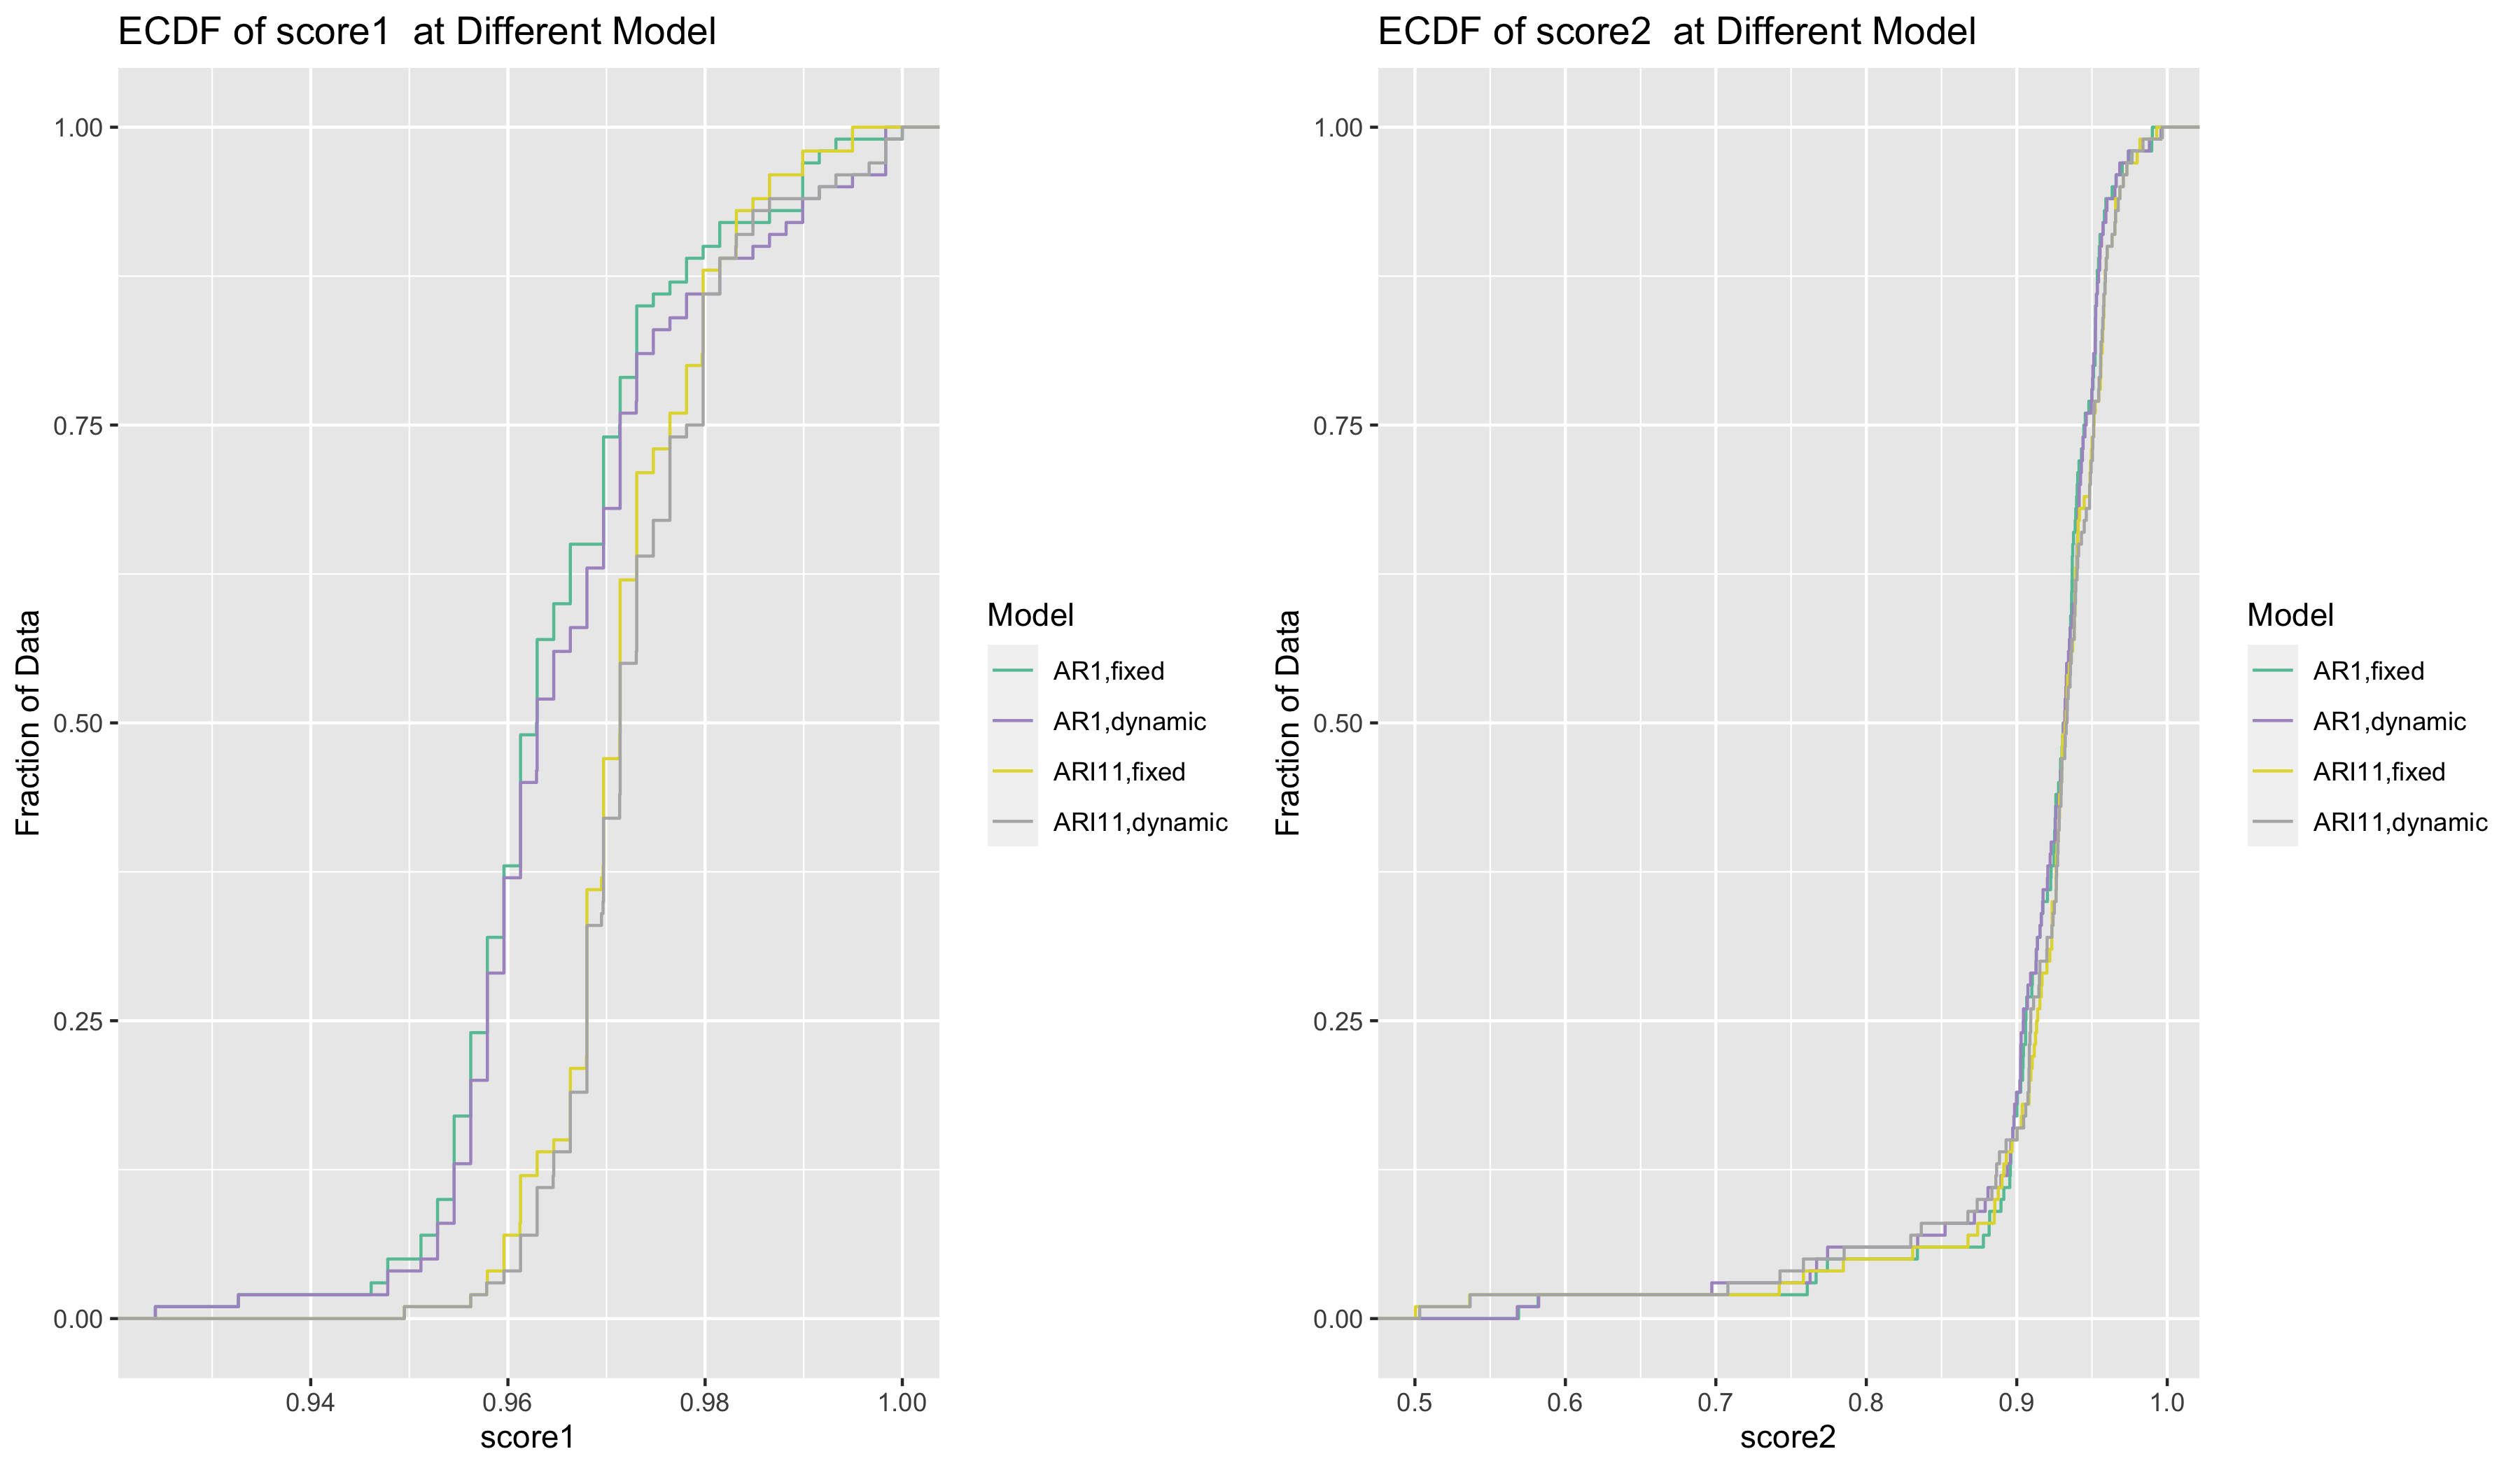
\includegraphics{images/ECDFofscoresatDifferentModelOfAR1,ARI11,fixed,dynamic.png}
    \label{fig:fig1.10.2}
\end{figure}

\begin{table}[htbp]
  \begin{center}
    \caption{Configuration and Result of Different Models Predicting Averages of Next Window with Online Training}
    \label{tab:tab1.10.2}
    \begin{tabular}{l|l|*{4}{c}}
      \textbf{model} & \textbf{training policy} & \textbf{score 1} & \textbf{score 1 weight} & \textbf{score 2} & \textbf{score 2 weight} \\
      \hline
      AR1 & fixed & 0.9646 & 59398 & 0.9173 & 59400\\
      AR1 & dynamic & 0.9662 & 59397 & 0.9149 & 59400\\
      ARI11 & fixed & 0.9718 & 59386 & 0.9192 & 59400\\
      ARI11 & dynamic & 0.9731 & 59387 & 0.9168 & 59400\\
    \end{tabular}
  \end{center}
\end{table}

\begin{figure}
    \caption{ECDF of Scores for Different Models Predicting Averages of Next Window with Offline Training}
    \centering
    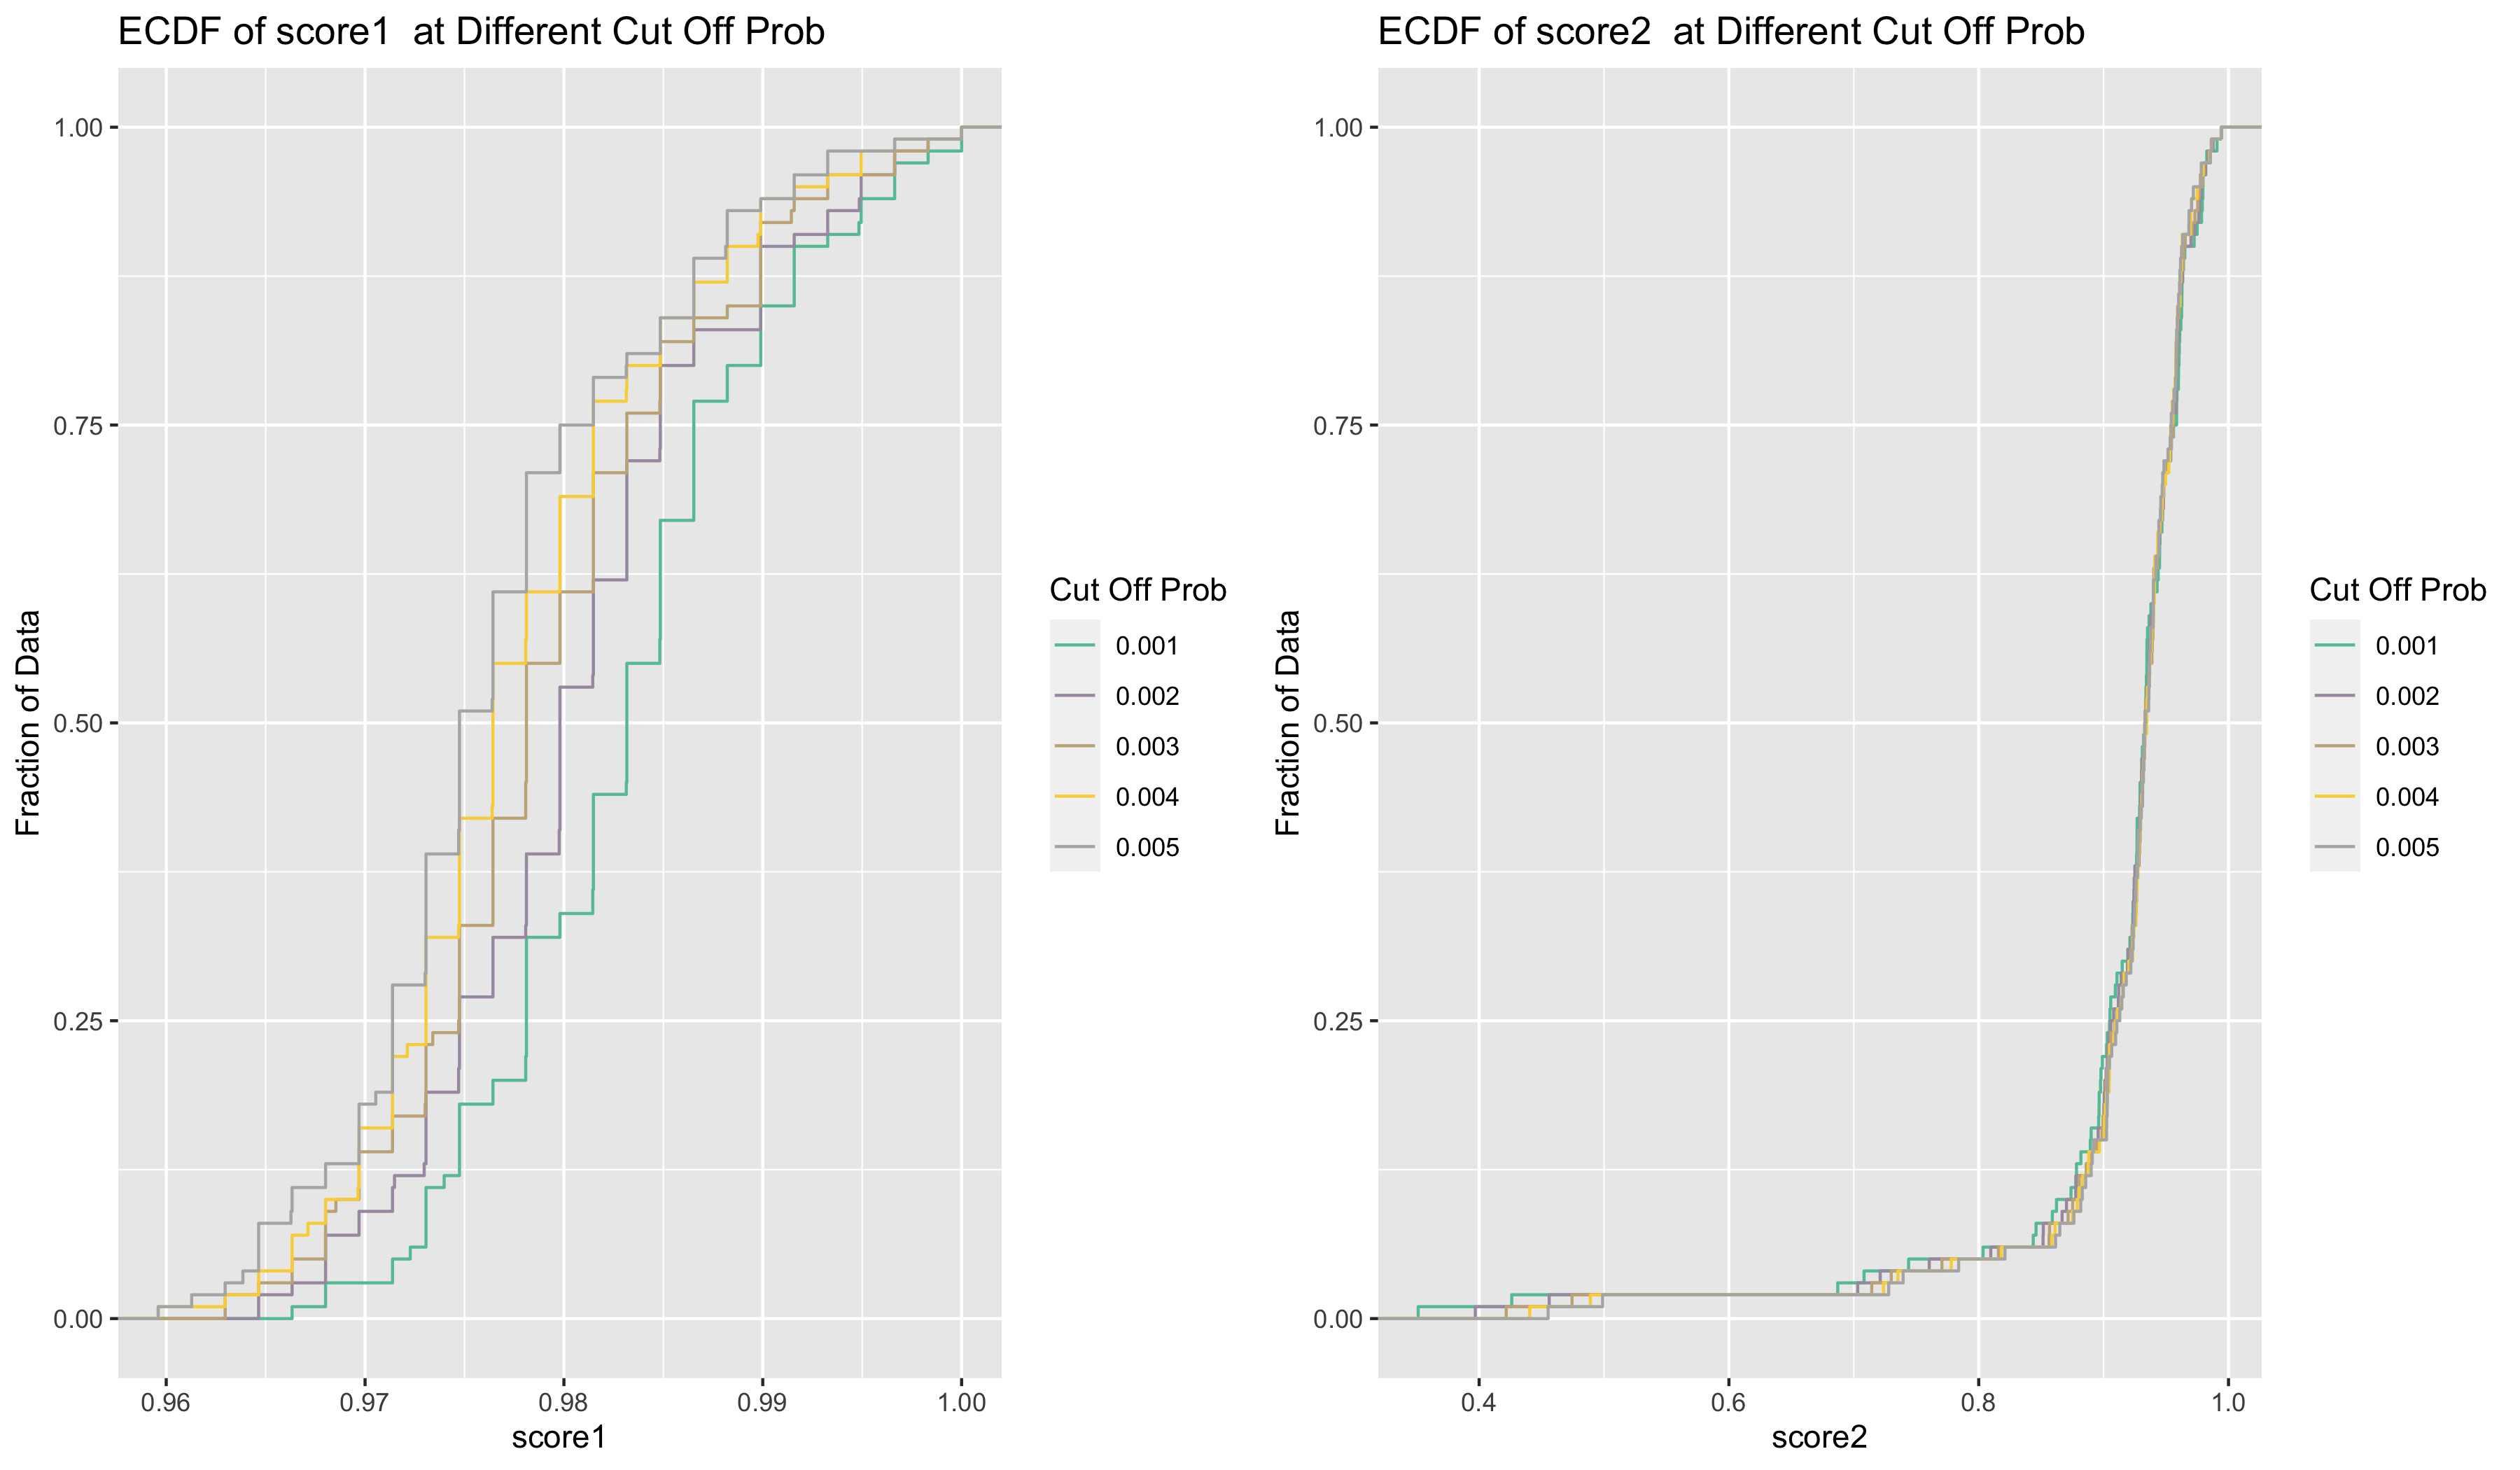
\includegraphics{images/ECDFofscoresatDifferentCutOffProbOfARI11,fixed.png}
    \label{fig:fig1.10.3}
\end{figure}

\begin{table}[htbp]
  \begin{center}
    \caption{Configuration and Result of Different Cut-off Probability Predicting Averages of Next Window with Fixed Online Training}
    \label{tab:tab1.10.3}
    \begin{tabular}{l|*{4}{c}}
      \textbf{cut off probability} & \textbf{score 1} & \textbf{score 1 weight} & \textbf{score 2} & \textbf{score 2 weight} \\
      \hline
      0.001 & 0.9831 & 59271 & 0.9139 & 59400\\
      0.002 & 0.9806 & 59310 & 0.9161 & 59400\\
      0.003 & 0.9792 & 59332 & 0.9174 & 59400\\
      0.004 & 0.9777 & 59350 & 0.9181 & 59400\\
      0.005 & 0.9766 & 59360 & 0.9186 & 59400\\
    \end{tabular}
  \end{center}
\end{table}

\subsubsection{Comparison Against Autopilot}

\begin{figure}
    \caption{Examples of Reconstructed Traces with Different Methods}
    \centering
    \includegraphics{images/}
    \label{fig:fig1.11.1}
\end{figure}

\begin{table}[htbp]
  \begin{center}
    \caption{Configuration and Result of Different j-quantile for Predicting Maximum of Next 5min Window Using Autopilot}
    \label{tab:tab1.11.1}
    \begin{tabular}{l|l|*{4}{c}}
      \textbf{reconstruct method} & \textbf{j} & \textbf{score 1} & \textbf{score 1 weight} & \textbf{score 2} & \textbf{score 2 weight} \\
      \hline
      Version 1 & 0.001 & 0.9969 & 414249 & 0.2298 & 716235\\
      Version 1 & 0.010 & 0.9834 & 614705 & 0.5077 & 716235\\
      Version 1 & 0.050 & 0.9385 & 678510 & 0.7093 & 716235\\
      Version 2 & 0.001 & 0.0000 & 000000 & 0.0000 & 716235\\
      Version 2 & 0.010 & 0.0000 & 000000 & 0.0000 & 716235\\
      Version 2 & 0.050 & 0.0000 & 000000 & 0.0000 & 716235\\
    \end{tabular}
  \end{center}
\end{table}

\begin{table}[htbp]
  \begin{center}
    \caption{Configuration and Result of Different half-life for Predicting Maximum of Next 5min Window Using Autopilot}
    \label{tab:tab1.11.2}
    \begin{tabular}{l|l|*{4}{c}}
      \textbf{reconstruct method} & \textbf{half-life} & \textbf{score 1} & \textbf{score 1 weight} & \textbf{score 2} & \textbf{score 2 weight} \\
      \hline
      Version 1 & 3h & 0.9821 & 623970 & 0.5447 & 716235\\
      Version 1 & 6h & 0.9830 & 619511 & 0.5267 & 716235\\
      Version 1 & 12h & 0.9834 & 614705 & 0.5077 & 716235\\
      Version 2 & 3h & 0.0000 & 000000 & 0.0000 & 716235\\
      Version 2 & 6h & 0.0000 & 000000 & 0.0000 & 716235\\
      Version 2 & 12h & 0.0000 & 000000 & 0.0000 & 716235\\
    \end{tabular}
  \end{center}
\end{table}

\begin{table}[htbp]
  \begin{center}
    \caption{Configuration and Result of Different Combination of window sizes and half-lifes for Predicting Maximum of Next Window Using Autopilot}
    \label{tab:tab1.11.4}
    \begin{tabular}{l|l|l|*{4}{c}}
      \textbf{reconstruct method} & \textbf{window size} & \textbf{half-life} & \textbf{score 1} & \textbf{score 1 weight} & \textbf{score 2} & \textbf{score 2 weight} \\
      \hline
      Version 1 & 5min & 3h & 0.9834 & 614705 & 0.5077 & 716235\\
      Version 1 & 1h & 0.9803 & 647914 & 0.5348 & 716235\\
      Version 1 & 3h & 0.9774 & 676506 & 0.5512 & 716235\\
      Version 2 & 10 & 0.0000 & 000000 & 0.0000 & 716235\\
      Version 2 & 20 & 0.0000 & 000000 & 0.0000 & 716235\\
      Version 2 & 50 & 0.0000 & 000000 & 0.0000 & 716235\\
    \end{tabular}
  \end{center}
\end{table}

\begin{table}[htbp]
  \begin{center}
    \caption{Configuration and Result of Different Number of Breaks for Predicting Maximum of Next 5min Window Using Autopilot}
    \label{tab:tab1.11.3}
    \begin{tabular}{l|l|*{4}{c}}
      \textbf{reconstruct method} & \textbf{number of breaks} & \textbf{score 1} & \textbf{score 1 weight} & \textbf{score 2} & \textbf{score 2 weight} \\
      \hline
      Version 1 & 10 & 0.9834 & 614705 & 0.5077 & 716235\\
      Version 1 & 20 & 0.9803 & 647914 & 0.5348 & 716235\\
      Version 1 & 50 & 0.9774 & 676506 & 0.5512 & 716235\\
      Version 2 & 10 & 0.0000 & 000000 & 0.0000 & 716235\\
      Version 2 & 20 & 0.0000 & 000000 & 0.0000 & 716235\\
      Version 2 & 50 & 0.0000 & 000000 & 0.0000 & 716235\\
    \end{tabular}
  \end{center}
\end{table}

\section{Prediction of Background Jobs}
\subsection{Main Motivation for the problem}

\begin{flushleft}
In the foreground part, the time series models do the prediction of the amount of available resource that can be scheduled in the next period of time, with the constraint for the overall survival rate. However, we do not know for sure how long a specific job will last in the machine. Therefore, we are aiming to predict the distribution of job's duration times, as a discrete probability vector:
$(p_1, p_2, ..., p_m)$, which can be used later with the models for the foreground part, to decide which job should be assigned to which machine.
\end{flushleft}

\begin{flushleft}
The methodology in this part can be decomposed into the following parts:
\begin{itemize}
    \item Discretization of the job duration times.
    \item Clustering of jobs
    \item Building probability vector within each cluster
    \item Diagnosis and Updating of the probability vectors
\end{itemize}
\end{flushleft}

\subsection{Discretization}

\begin{flushleft}
The reason that we need to do the discretization for job's duration time is that for each unique value of job's duration time, we need to correspond with a separate model in the foreground part. Since in practice we can only have finitely many models in each part, we need to discretize the duration times into finitely many distinct bins.

The first step for do a visualization of the unconditional job duration times, and decide the number and placement of our bins.

Based on this histogram Fig \ref{fig:fig2.2.1}, a reasonable bin vector will be:\newline $(0,1,2,6,10,14,18,22,26,30,50,80,205)$,
which covers the full range of job duration in this case, and places bins with smaller widths for region with greater density. Therefore, the discretized values of job duration will be\newline $(1,2,6,10,14,18,22,26,30,50,80,205)$ depending on which bin that job duration is in.
\end{flushleft}

\subsection{Clustering of jobs}

\begin{flushleft}
To make the probability vector a more accurate approximation for job's duration's distribution, jobs are assigned to different clusters. The clustering algorithms use job's features: priority, scheduling class, requested CPU, requested RAM and requested local disk space. There are two options available for the clustering algorithm.
\end{flushleft}

\subsubsection{Tree Method}

\begin{flushleft}
Using the training set, a \textbf{survival tree} or a \textbf{regression tree} that aims to predict the job's duration is fitted, and each terminal node will be regarded as a cluster for jobs. The survival tree treats each observation of the job's duration as a realization from a specific exponential distribution, with each terminal node in the tree represents a different type of exponential distribution, and seeks to maximize a likelihood criterion. The regression tree just treats each duration as a usual continuous numerical variable and seeks to minimize the sum of squares. The number of clusters will be the number of terminal nodes in the tree, so it does not need to be specified beforehand.
\end{flushleft}

\begin{flushleft}
\textbf{minsize}: Minsize used when the tree method is selected for the clustering. It specifies the minimum number of observations in each terminal node of the tree. To make sure later the probability vector in each cluster is estimated accurately, it is necessary to make sure that there are enough observations in each cluster.
\end{flushleft}

\subsubsection{Gaussian Mixture Model Method}

\begin{flushleft}
Different from the tree method above, the GMM method does the clustering without looking at the response variable duration time. This method simply treats the features of each job are multivariate normally distributed, and models the whole data-set as a mixture of normal distributions. To use this algorithm, it is necessary to know the number of clusters in the data set. So without this information, the algorithm will automatically try for a bunch of numbers and select the one with the optimal BIC value.
\end{flushleft}

\begin{flushleft}
\textbf{upperlimBIC}: Upper Limit BIC used when the GMM method is selected. It specifies the maximum number of cluster that the algorithm will try when it is selecting the number of clusters in the model.
\end{flushleft}

\subsection{Building probability vector}

\begin{flushleft}
After obtaining a model for the clustering, and a clustered training set, a probability vector can be estimated in each cluster by looking at the empirical distribution(histogram). For example, if we discretized the job duration time into m discrete values, and found out that there are k clusters after the clustering, then we are looking for a list of k vectors, each with m components, i.e.:
$\{(p_{i1}, p_{i2}, ..., p_{im}) : i \in (1,...,k)\}$. The value of $p_{ij}$ can be interpreted as the probability that a job in cluster i, has duration time $t_j$ (the j-th distinct duration time after discretization).
\end{flushleft}

\subsection{Diagnosis and Updating}

\begin{flushleft}
To test the accuracy of probability vectors we obtained from training set, we use the probability vectors obtained from the testing set, by measuring the average squared error weighted by the number of observations in each labeled testing set. (For this measure to make sense, we need the number of observations in the unconditional testing set to be large enough, but not necessary for each labeled testing set, as they are already weighted).
For example, denote the number of observations in the (unconditional) testing set as $T$, and the number of observations in cluster i in the testing set as $T_i$, and let $\{(q_{i1}, q_{i2}, ..., q_{im}) : i \in (1,...,k)\}$ be the list of probability vectors obtained from the testing set, then our measure of discrepancy will be:
\end{flushleft}

\begin{flushleft}
\begin{equation}
\centering
        \sum_{i = 1} ^{k} \frac{T_i}{T} \sum_{j = 1}^{m} \frac{(q_{ij} - p_{ij})^2}{m}
\end{equation}
\end{flushleft}

\begin{flushleft}
When this value is too large, it might be that users have now changed their usual behavior, and we need to gradually adopt their new behavior by updating our probability vector. It could be done by randomly dropping observations from the unconditional training set, and replace these observations by the testing set we used and recompute the probability vector.
\end{flushleft}

\subsection{Appendix}

\subsubsection{Discretization}

\begin{figure}[htbp]
\caption{Unconditional Histogram of Job Duration}
\centering
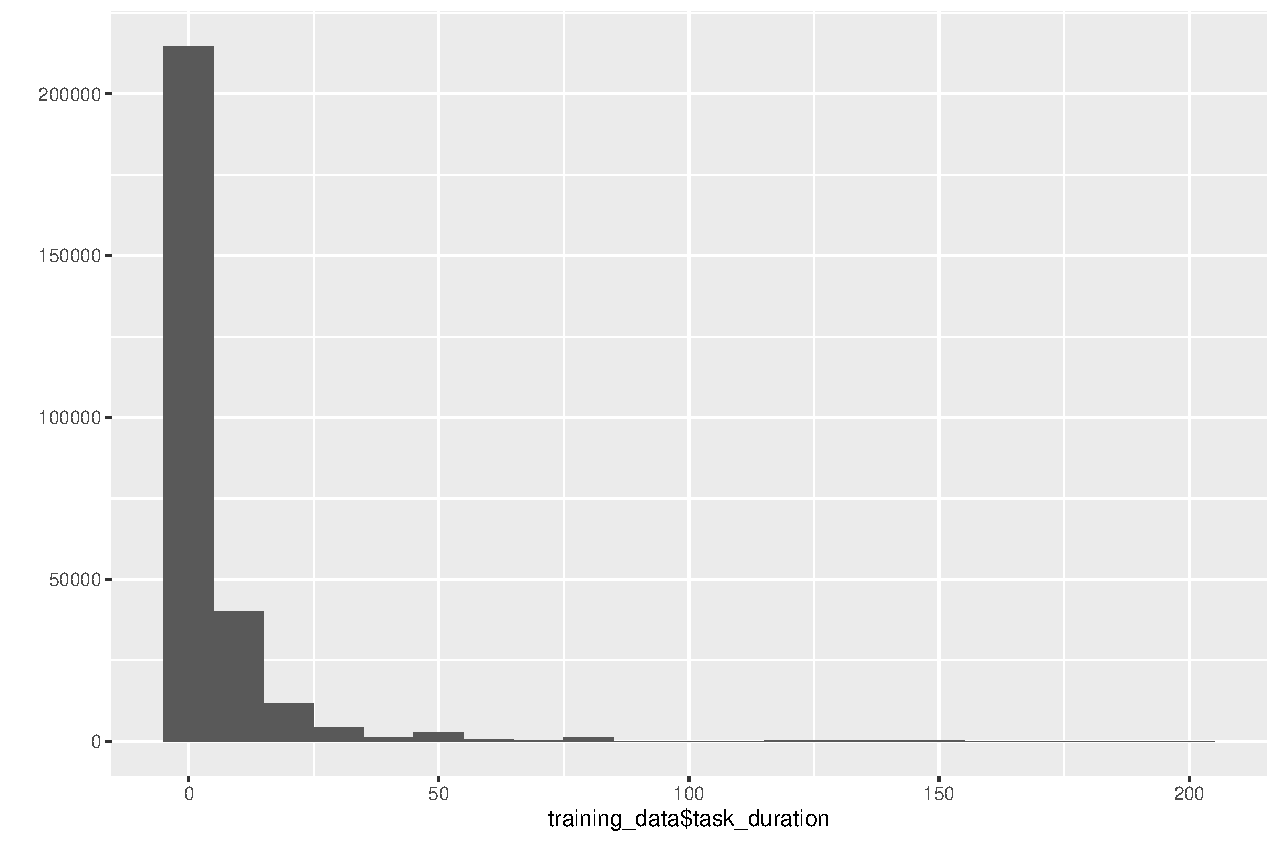
\includegraphics[width = 0.8\textwidth]{uncondional_hist}
\label{fig:fig2.2.1}
\end{figure}

\section{Combining Predictions of Two Parts}
\subsection{Overview of Current method}
\begin{flushleft}
Our current method of combining foreground jobs model and background jobs model can be summarized as following:

\begin{enumerate}[Step 1:]
    \item Given a job, we use the clustering model from the background part to identify which cluster it is in. Let its requested CPU be $R$.
    \item Using the probability vector of this cluster from background part, we know the probability of this job finishing at different times. Let's suppose that the probability vector is $P = (p_{1}, ..., p_{m})$
    \item There will be also m models running on the foreground part, and each of them will have a aggregation time correspond to a component of the discretized job duration times. Each of these models will give a one-step forward prediction for the available resource on the machine. Call this vector of one step predictions as $(r_1, ... , r_m)$.
    \item Notice that $r_i$ can be interpreted as the amount of available resource given that time T equals $t_i$. So the expected available resource for this job is computed as $U = \sum_{i=1}^{m} p_i r_i$.
    \item For the j-th machine, we can compute the probability that the i-th job can be finished, by summing over the components in the probability vector such that $r_j \geq R_i$. If this sum is greater than the specified threshold (a default value is $\sqrt{99}$ percent), we call this machine is plausible for the job. 
    \item For the j-th machine, compute the cost $D_j$ as:$U_j - R$ if $R \leq U_j$, and $\infty$ otherwise. Then among all the plausible machines, we will choose to allocate a job to the machine with minimum cost.
\end{enumerate}

\textbf{Order of Scheduling Jobs}: Since scheduling multiple jobs on multiple machines with some capacities is a multi-dimensional knapsack problem which is an NP hard problem. A simple approximation algorithm we proposed is to order the jobs by their requested CPU and consecutively scheduled (following Step 4, Step 5 and Step 6).

\textbf{Killing Jobs}: Sometimes outliers or irregular fluctuations may occur and the foreground CPU resource may interfere with background scheduled jobs. In this case, we need to at least free up the CPU resource scheduled subtracted by CPU resource actually available, denoted by $C$.

In order to find the suitable jobs to kill to minimize the number of jobs being killed while also minimizing CPU utilization lost, a two-step dynamic programming algorithm is implemented: First, order the current scheduled jobs by their requested CPU in descending order, then by consecutively removing the jobs in order, we can find the minimum number of jobs that needs to be killed in order to accommodate the spike in foreground CPU resource. Second, we consecutively select the minimum number of jobs to kill with minimum resource occupied of $C$ at this time of while minimizing the loss of CPU resource as the result of killing such selected jobs, that is, the sum of product of CPU resource requested and the amount of time the job has been running. A dynamic programming algorithm in the second step would significantly reduce the run time.

It is also noticeable that the running time of the above is approximately $O(n^k)$ where $n$ is the number of jobs active at any timestamp, $k$ is an integer greater than $0$ as the number of jobs that needs to be killed. Another alternative is simply order the jobs by their requested CPU in descending order and select jobs from top of the list to kill. This approach significantly reduce the running time and does not have any impact on survival rate since the number of jobs being killed is exactly the same as dynamic programming algorithm described above, but the utilization rate will be lower since the whole purpose of the dynamic programming algorithm is to find smallest job to kill.

\textbf{Randomized Simulation}: There are two parts of the simulations that are random; the arrival time of the jobs are uniformly assigned across all simulation time length and the machine selected. In order to generate more stable results, each simulation is repeated at least 10 times and averaged as the final performance.
\end{flushleft}

\subsection{Simulation Study}

\begin{flushleft}
The purpose of these simulations is to deal with the case of how to allocate each job into the optimal machine (we want it to survive, but not to waste so much resource). We used the google data set for jobs, and the Microsoft data set for foreground predictions.
\end{flushleft}

\begin{flushleft}
The foreground setting of simulation is to use simple AR1 model with offline training strategy, with training size of 3000 data points and the length of simulation is 100 unit time (500 minutes). The background setting of simulation is to use ANOVA tree model on clustering and 5000 jobs as training set.
\end{flushleft}

\subsubsection{Arrival Rate}

\begin{flushleft}
Arrival rate refers to the number of jobs arrivals per unit of time. If all the jobs can be ideally scheduled onto the machines, the arrival rate is considered to be \textbf{sparse}, and if the jobs are competing for resources and a significant proportion of jobs cannot be scheduled eventually, then the arrival rate is considered to be \textbf{dense}.

\textbf{Load of Jobs}: The load of jobs is an indicator of how dense the arrival rate is for fixed choices of machines. It is simply the sum of CPU resource requested by all jobs times their running time divided by the resource available across all machines summed at all simulation time. When the load is close to $1$, a small proportion of the jobs may eventually fail to be scheduled, and when the load is much greater than $1$, the jobs are competing for resources and all machines can be presumed to be fully occupied at all time.

Table \ref{tab:tab3.2.1} shows that the performance of survival rate is not affected by the arrival rate or the load, the utilization becomes better as arrival rate increases because more choices of jobs becomes available at higher rates, and the algorithm may have better selections.

Another method of changing the ariival rate is to increase the simulation length, Table \ref{tab:tab3.2.2} shows that fixing the number of background jobs to be $5000$ as simulation length increases, the utilization decreases and 
\end{flushleft}

\subsubsection{Models for Background Jobs}

\begin{flushleft}
As described in the Tree Methods and GMM Methods in the previous section, we aim to compare the performance of simulation results using the three different models for clustering background jobs.
\end{flushleft}

\subsection{Appendix}

\subsubsection{Simulation Study}

\begin{table}[htbp]
  \begin{center}
    \caption{Combined Simulation of AR1 Model and ANOVA tree with Different Number of Jobs}
    \label{tab:tab3.2.1}
    \begin{tabular}{{l}|*{5}{c}}
      \textbf{job num} & \textbf{finished utilization} & \textbf{survival rate} & \textbf{load} & \textbf{unfinished rate} & \textbf{unscheduled rate} \\
      \hline
      1000 & 0.1185 & 0.9966 & 0.8077 & 0.0070 & 0.4038\\
      2000 & 0.1808 & 0.9956 & 1.5285 & 0.0024 & 0.5262\\
      3000 & 0.1877 & 0.9937 & 1.8106 & 0.0017 & 0.6019\\
      5000 & 0.2950 & 0.9965 & 2.7880 & 0.0015 & 0.6405\\
    \end{tabular}
  \end{center}
\end{table}

\begin{table}[htbp]
  \begin{center}
    \caption{Combined Simulation of AR1 Model and ANOVA tree with Different Length of Simulation}
    \label{tab:tab3.2.2}
    \begin{tabular}{{l}|*{5}{c}}
      \textbf{sim length} & \textbf{finished utilization} & \textbf{survival rate} & \textbf{load} & \textbf{unfinished rate} & \textbf{unscheduled rate} \\
      \hline
      100 & 0.2950 & 0.9965 & 2.7880 & 0.0015 & 0.6405\\
      200 & 0.2490 & 0.9953 & 1.3927 & 0.0016 & 0.5003\\
      500 & 0.2465 & 0.9923 & 0.5649 & 0.0009 & 0.1608\\
      1000 & 0.1645 & 0.9926 & 0.2828 & 0.0005 & 0.1435\\
      1500 & 0.0938 & 0.9965 & 0.1857 & 0.0003 & 0.1897\\
    \end{tabular}
  \end{center}
\end{table}

\begin{table}[htbp]
  \begin{center}
    \caption{Combined Simulation of AR1 Model and Different Models}
    \label{tab:tab3.2.3}
    \begin{tabular}{{l}|*{5}{c}}
      \textbf{sim length} & \textbf{finished utilization} & \textbf{survival rate} & \textbf{load} & \textbf{unfinished rate} & \textbf{unscheduled rate} \\
      \hline
      anova tree & 0.2950 & 0.9965 & 2.7880 & 0.0015 & 0.6405\\
      survival tree & 0.2993 & 0.9956 & 2.5562 & 0.0011 & 0.5568\\
    \end{tabular}
  \end{center}
\end{table}

\begin{figure}[htbp]
\caption{Histogram of percent performance}
\centering
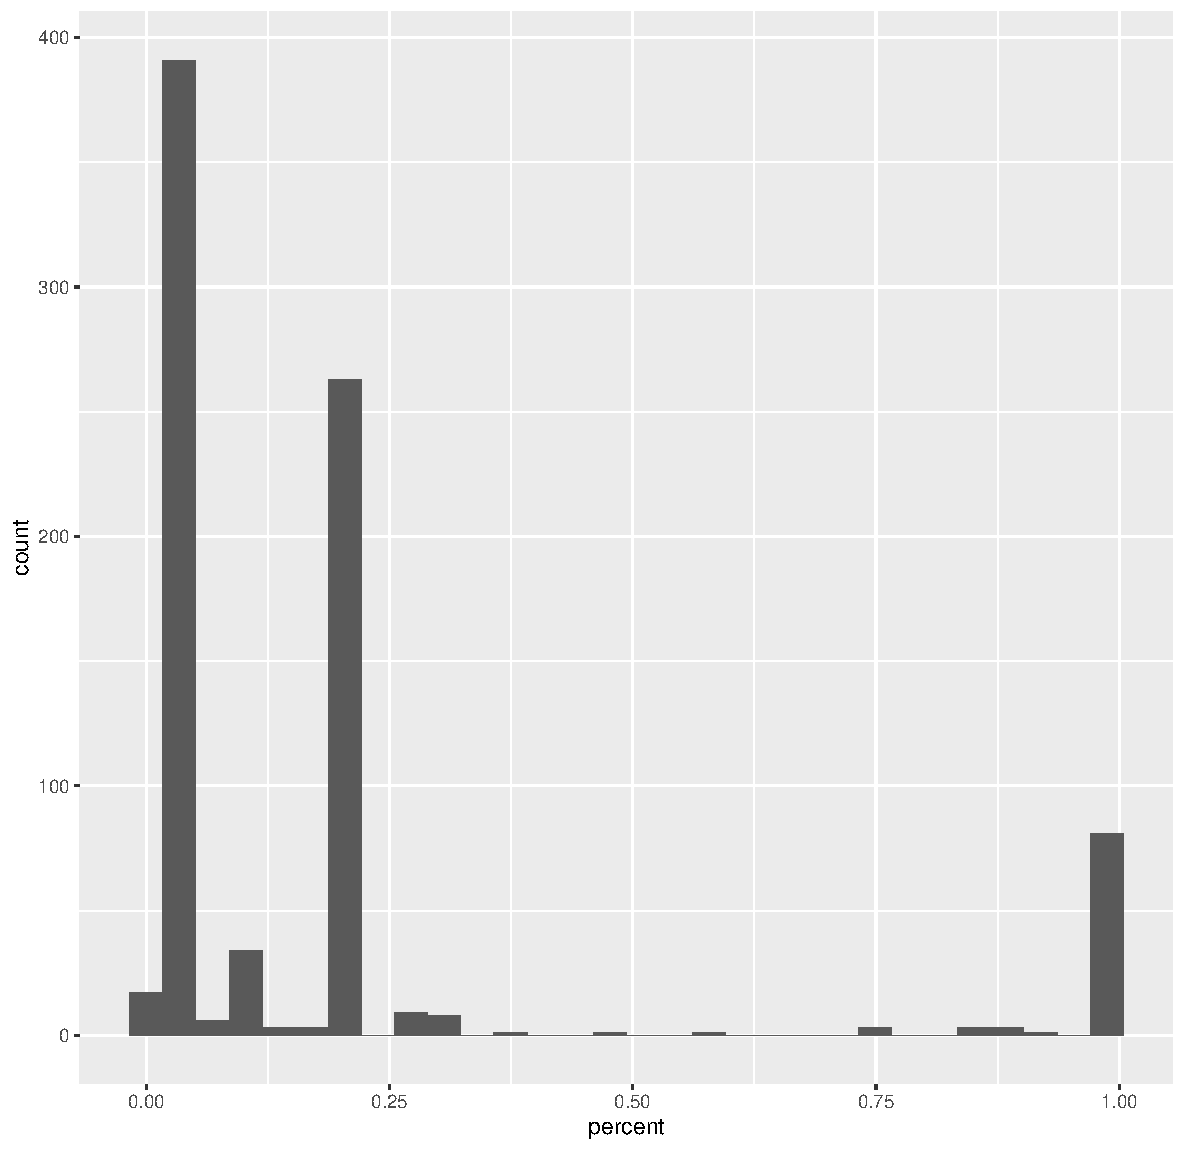
\includegraphics[width = 0.8\textwidth]{sur_tree}
\end{figure}

\end{document}
